%%
%% This is file `sample-sigconf-authordraft.tex',
%% generated with the docstrip utility.
%%
%% The original source files were:
%%
%% samples.dtx  (with options: `all,proceedings,bibtex,authordraft')
%% 
%% IMPORTANT NOTICE:
%% 
%% For the copyright see the source file.
%% 
%% Any modified versions of this file must be renamed
%% with new filenames distinct from sample-sigconf-authordraft.tex.
%% 
%% For distribution of the original source see the terms
%% for copying and modification in the file samples.dtx.
%% 
%% This generated file may be distributed as long as the
%% original source files, as listed above, are part of the
%% same distribution. (The sources need not necessarily be
%% in the same archive or directory.)
%%
%%
%% Commands for TeXCount
%TC:macro \cite [option:text,text]
%TC:macro \citep [option:text,text]
%TC:macro \citet [option:text,text]
%TC:envir table 0 1
%TC:envir table* 0 1
%TC:envir tabular [ignore] word
%TC:envir displaymath 0 word
%TC:envir math 0 word
%TC:envir comment 0 0
%%
%%
%% The first command in your LaTeX source must be the \documentclass
%% command.
%%
%% For submission and review of your manuscript please change the
%% command to \documentclass[manuscript, screen, review]{acmart}.
%%
%% When submitting camera ready or to TAPS, please change the command
%% to \documentclass[sigconf]{acmart} or whichever template is required
%% for your publication.
%%
%%
% \documentclass[sigconf,authorversion]{acmart}
%\documentclass[sigconf,anonymous,review]{acmart}
% \documentclass[acmtog,anonymous,review]{acmart}
\documentclass[acmtog, authorversion]{acmart}

\makeatother

\acmSubmissionID{915}
\usepackage{graphicx}
\usepackage{booktabs}

\usepackage{multirow}
\usepackage{makecell}
\usepackage{arydshln}
\usepackage{enumitem}
% \usepackage{bibunits}

\newcommand{\TODO}[1]{\textbf{\color{red}[TODO: #1]}}

%%
%% \BibTeX command to typeset BibTeX logo in the docs
\AtBeginDocument{%
  \providecommand\BibTeX{{%
    Bib\TeX}}}

%% Rights management information.  This information is sent to you
%% when you complete the rights form.  These commands have SAMPLE
%% values in them; it is your responsibility as an author to replace
%% the commands and values with those provided to you when you
%% complete the rights form.
\setcopyright{acmlicensed}
\acmJournal{TOG}
\copyrightyear{2024}
\acmYear{2024} \acmVolume{43} \acmNumber{6} \acmArticle{} \acmMonth{12}
% \acmDOI{10.1145/3687975}
\acmDOI{10.1145/3687975}



% TOG prefers author-name bib system with square brackets
\citestyle{acmauthoryear}
%% These commands are for a PROCEEDINGS abstract or paper.
% \acmConference[Conference acronym 'XX]{Make sure to enter the correct
%   conference title from your rights confirmation emai}{June 03--05,
%   2018}{Woodstock, NY}
%%
%%  Uncomment \acmBooktitle if the title of the proceedings is different
%%  from ``Proceedings of ...''!
%%
%%\acmBooktitle{Woodstock '18: ACM Symposium on Neural Gaze Detection,
%%  June 03--05, 2018, Woodstock, NY}
% \acmISBN{978-1-4503-XXXX-X/18/06}


%%
%% Submission ID.
%% Use this when submitting an article to a sponsored event. You'll
%% receive a unique submission ID from the organizers
%% of the event, and this ID should be used as the parameter to this command.
%%\acmSubmissionID{123-A56-BU3}

%%
%% For managing citations, it is recommended to use bibliography
%% files in BibTeX format.
%%
%% You can then either use BibTeX with the ACM-Reference-Format style,
%% or BibLaTeX with the acmnumeric or acmauthoryear sytles, that include
%% support for advanced citation of software artefact from the
%% biblatex-software package, also separately available on CTAN.
%%
%% Look at the sample-*-biblatex.tex files for templates showcasing
%% the biblatex styles.
%%

%%
%% The majority of ACM publications use numbered citations and
%% references.  The command \citestyle{authoryear} switches to the
%% "author year" style.
%%
%% If you are preparing content for an event
%% sponsored by ACM SIGGRAPH, you must use the "author year" style of
%% citations and references.
%% Uncommenting
%% the next command will enable that style.
%%\citestyle{acmauthoryear}


%%
%% end of the preamble, start of the body of the document source.
\begin{document}
% \begin{sloppypar}

%%
%% The "title" command has an optional parameter,
%% allowing the author to define a "short title" to be used in page headers.
%\title{StyleCrafter: Enhancing Stylized Text-to-Video Generation with Style Adapter}
\title{StyleCrafter: Taming Stylized Video Diffusion with Reference-Augmented Adapter Learning}

%%
%% The "author" command and its associated commands are used to define
%% the authors and their affiliations.
%% Of note is the shared affiliation of the first two authors, and the
%% "authornote" and "authornotemark" commands
%% used to denote shared contribution to the research.
\author{Gongye Liu}
\affiliation{
  \institution{Tsinghua University}
  \city{Shenzhen}
  \country{China}
}
\email{lgy22@mails.tsinghua.edu.cn}


\author{Menghan Xia}
\authornote{Corresponding authors}
\author{Yong Zhang}
\author{Haoxin Chen}
\affiliation{
  \institution{Tencent AI Lab}
  \city{Shenzhen}
  \country{China}
}
\email{menghanxyz@gmail.com}
\email{zhangyong201303@gmail.com}
\email{jszxchx@gmail.com}

\author{Jinbo Xing}
\affiliation{%
  \institution{The Chinese University of Hong Kong}
  \city{Hong Kong}
  \country{China}
}
\email{jbxing@cse.cuhk.edu.hk}

\author{Yibo Wang}
\affiliation{%
  \institution{Tsinghua University}
  \city{Shenzhen}
  \country{China}
}
\email{wyb22@mails.tsinghua.edu.cn}

\author{Xintao Wang}
\author{Ying Shan}
\affiliation{%
  \institution{Tencent AI Lab}
  \city{Shenzhen}
  \country{China}
}
\email{xintao.alpha@gmail.com}
\email{yingsshan@tencent.com}

\author{Yujiu Yang}
\authornotemark[1]
\affiliation{%
  \institution{Tsinghua University}
  \city{Shenzhen}
  \country{China}
}
\email{yang.yujiu@sz.tsinghua.edu.cn}



%%
%% By default, the full list of authors will be used in the page
%% headers. Often, this list is too long, and will overlap
%% other information printed in the page headers. This command allows
%% the author to define a more concise list
%% of authors' names for this purpose.
% \renewcommand{\shortauthors}{Trovato et al.}

%%
%% The abstract is a short summary of the work to be presented in the
%% article.
\begin{abstract}

Text-to-video (T2V) models have shown remarkable capabilities in generating diverse videos. However, they struggle to produce user-desired artistic videos due to (i) text's inherent clumsiness in expressing specific styles and (ii) the generally degraded style fidelity. To address these challenges, we introduce StyleCrafter, a generic method that enhances pre-trained T2V models with a style control adapter, allowing video generation in any style by feeding a reference image.
Considering the scarcity of artistic video data, we propose to first train a style control adapter using style-rich image datasets, then transfer the learned stylization ability to video generation through a tailor-made finetuning paradigm. 
To promote content-style disentanglement, we employ carefully designed data augmentation strategies to enhance decoupled learning. Additionally, we propose a scale-adaptive fusion module to balance the influences of text-based content features and image-based style features, which helps generalization across various text and style combinations.
StyleCrafter efficiently generates high-quality stylized videos that align with the content of the texts and resemble the style of the reference images. Experiments demonstrate that our approach is more flexible and efficient than existing competitors.
Project page: \url{https://gongyeliu.github.io/StyleCrafter.github.io/}

\end{abstract}

%%
%% The code below is generated by the tool at http://dl.acm.org/ccs.cfm.
%% Please copy and paste the code instead of the example below.
%%
\begin{CCSXML}
<ccs2012>
 <concept>
  <concept_id>00000000.0000000.0000000</concept_id>
  <concept_desc>Do Not Use This Code, Generate the Correct Terms for Your Paper</concept_desc>
  <concept_significance>500</concept_significance>
 </concept>
 <concept>
  <concept_id>00000000.00000000.00000000</concept_id>
  <concept_desc>Do Not Use This Code, Generate the Correct Terms for Your Paper</concept_desc>
  <concept_significance>300</concept_significance>
 </concept>
 <concept>
  <concept_id>00000000.00000000.00000000</concept_id>
  <concept_desc>Do Not Use This Code, Generate the Correct Terms for Your Paper</concept_desc>
  <concept_significance>100</concept_significance>
 </concept>
 <concept>
  <concept_id>00000000.00000000.00000000</concept_id>
  <concept_desc>Do Not Use This Code, Generate the Correct Terms for Your Paper</concept_desc>
  <concept_significance>100</concept_significance>
 </concept>
</ccs2012>
\end{CCSXML}

\ccsdesc[500]{Computing methodologies~Computer Vision}

\keywords{Diffusion Model, Stylized Generation, Image/Video Synthesis}

\begin{teaserfigure}
  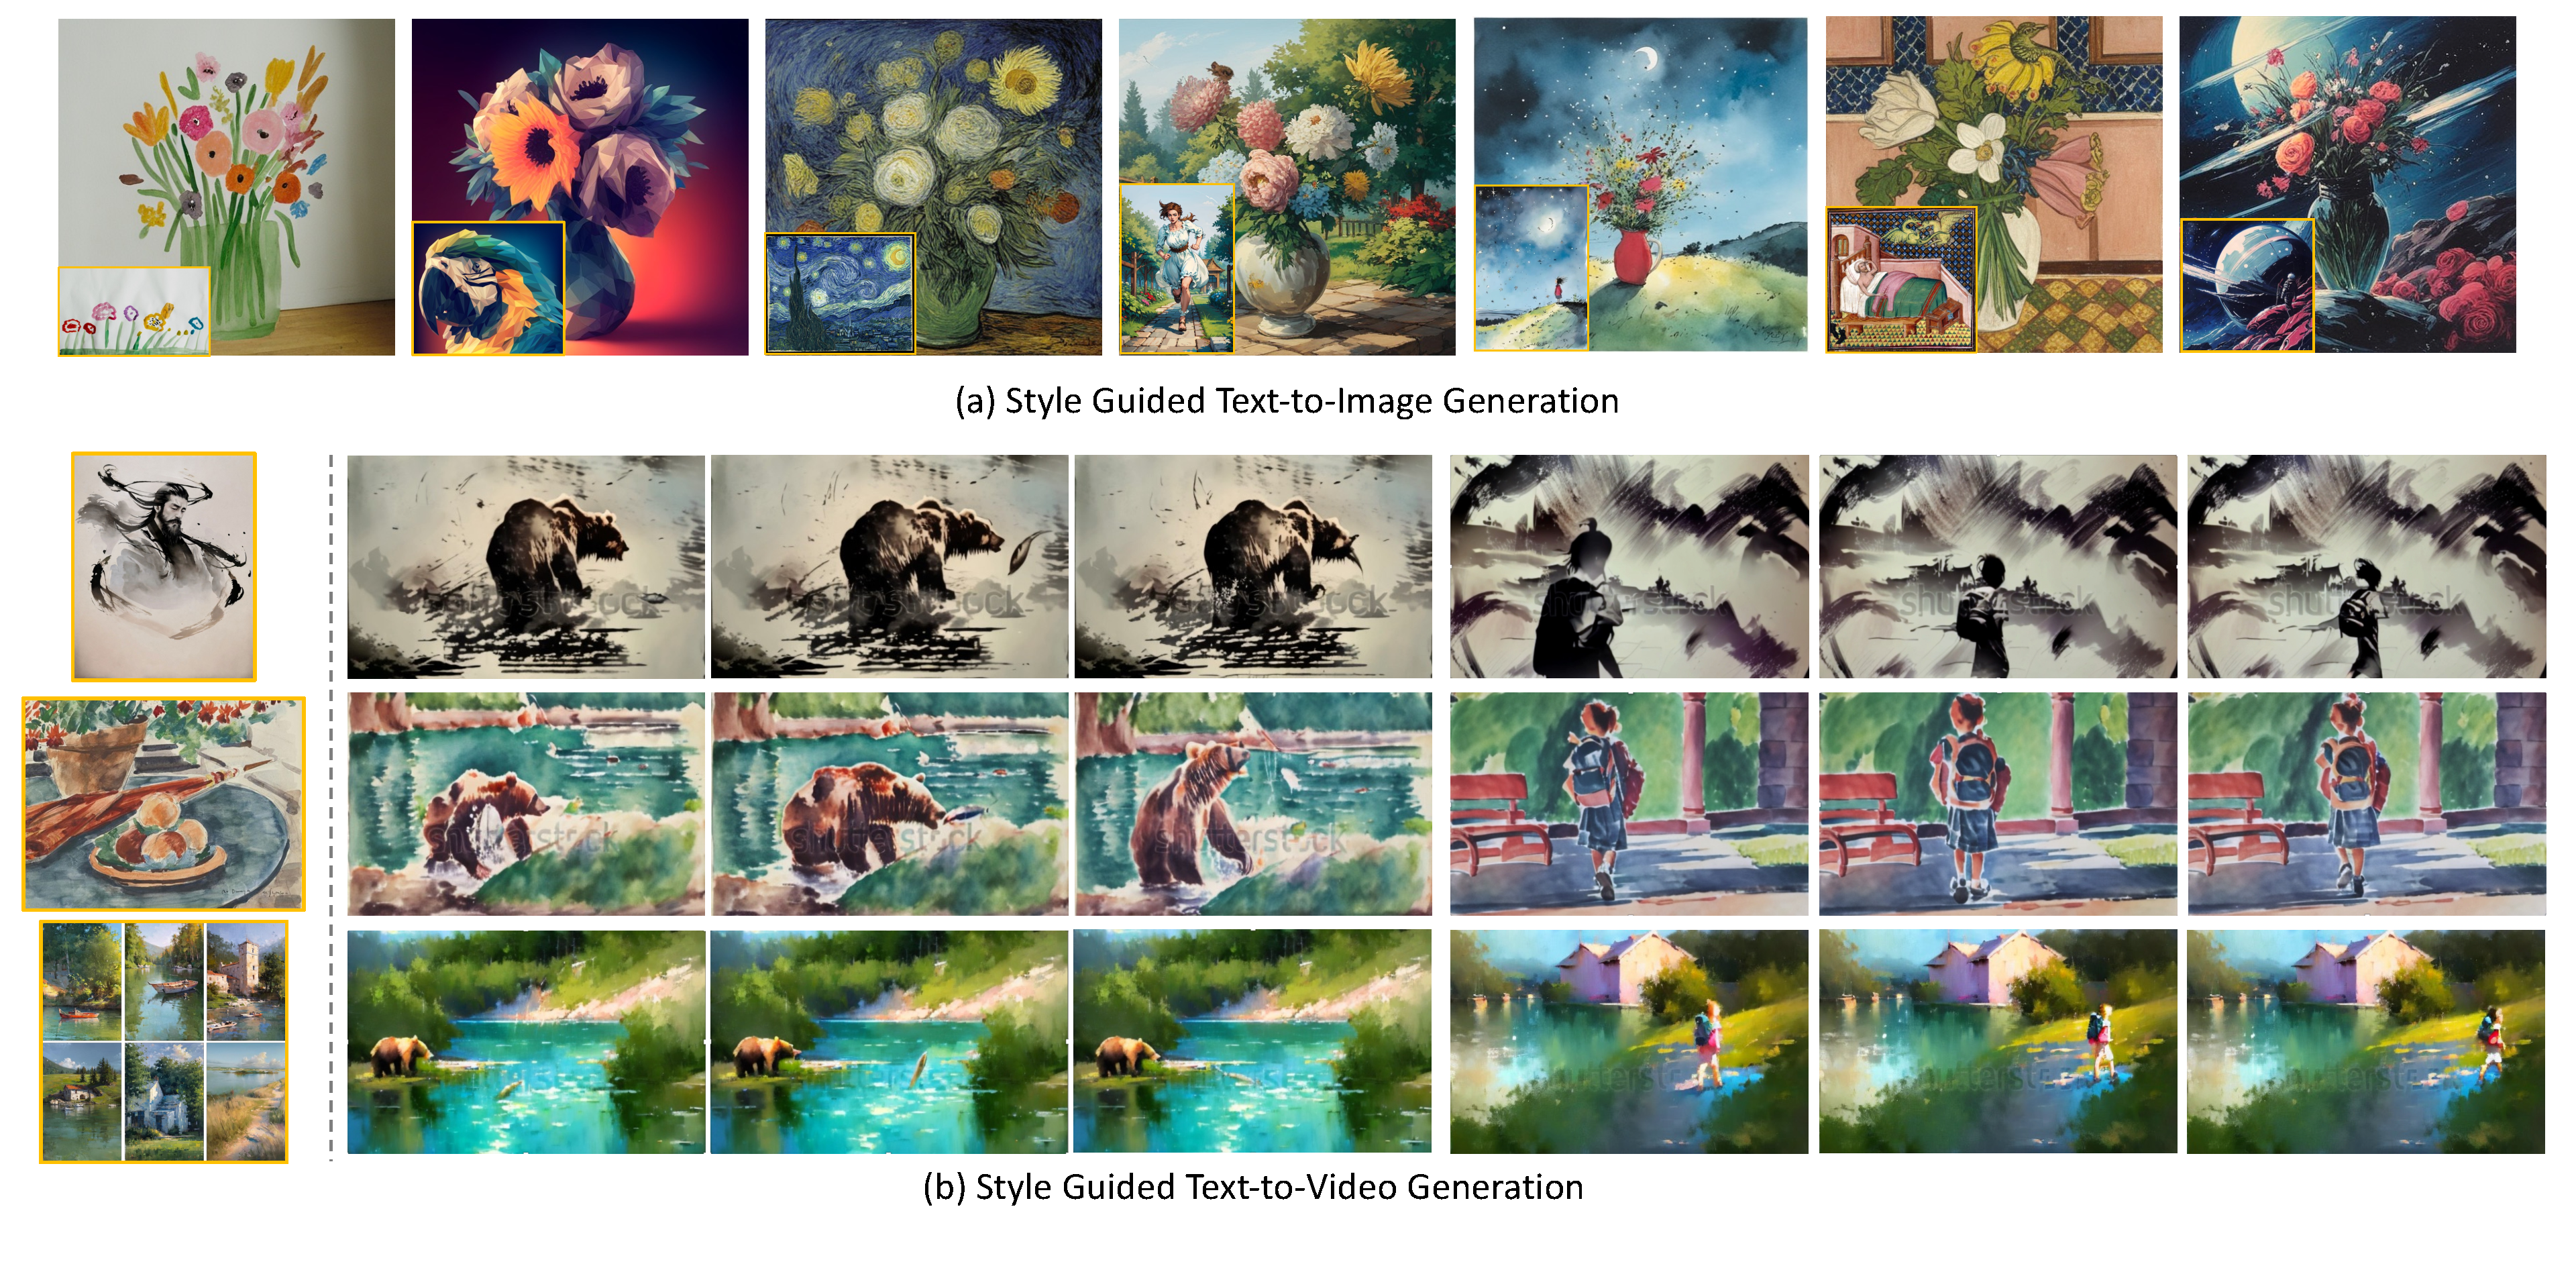
\includegraphics[width=\textwidth]{figures/teaser.pdf}
  \vspace{-3em}
  \caption{Stylized Generation Results Produced by StyleCrafter}
  \Description{Stylized Generation Results Produced by StyleCrafter}
  % \vspace{-2em}
  \label{fig:teaser}
\end{teaserfigure}

% \received{20 February 2007}
% \received[revised]{12 March 2009}
% \received[accepted]{5 June 2009}

%%
%% This command processes the author and affiliation and title
%% information and builds the first part of the formatted document.
\maketitle

\begin{sloppypar}

%%%%%% for TOG %%%%%% 
% % \begin{bibunit}
% %---------------------------------
\section{Introduction}
\label{sec:intro}
%---------------------------------


The popularity of powerful diffusion models has led to remarkable progress in the field of content generation. For instance, text-to-image (T2I) models are capable of generating diverse and vivid images from text prompts, encompassing various visual concepts. This great success can be attributed not only to the advancement of models but also to the availability of various image data over the Internet.
Constrastingly, text-to-video (T2V) models fall short of the data categories especially in styles, since existing videos predominantly feature photorealism. While these strategies, like initializing weights from well-trained T2I models or joint training with image and video datasets, can help mitigate this issue, the generated stylized videos generally suffer from degraded style fidelity. 
% Therefore, in addition to the classic problem of \textbf{style-content decoupling} in style transfer/preserving, stylized video generation also grapples with challenges including \textbf{a scarcity of stylized video data} and the \textbf{limited capabilities of T2V base models}.
Although significant success has been achieved in style transfer/preservation in T2I generation, the field of stylized video generation remains largely unexplored,
and effective solutions are yet to be discovered.
% As one of the pioneers, AnimateDiff~\cite{guo2023animatediff} can make impressive stylized videos by combining personalized T2I models~\cite{hu2022lora} (i.e. LoRA-tuned\cite{hu2022lora} or Dreambooth-tuned\cite{dreambooth} on Stable Diffusion\cite{ldm}) with pre-trained temporal blocks. However, each style requires additional finetuning on a small set of examples, which is inefficient and unable to support any style.

% \begin{figure}[!t]
%     \centering
%     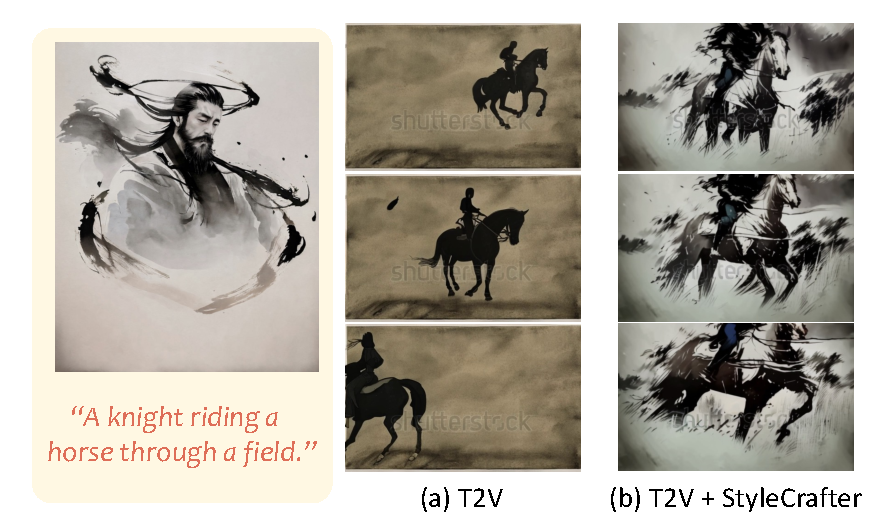
\includegraphics[width=\linewidth]{figures/motivation.pdf}\vspace{-0.5em}
%     \caption{Effect of adding style adapter to T2V models. (a) and (b) are results of Stable Diffusion~\cite{ldm} and VideoCrafter~\cite{chen2023videocrafter}. (c) is the result of VideoCrafter equipped with a style adapter. The content text prompt is "\textit{A knight riding a horse through the field}". For (a) and (b), the style prompt is generated from the style image using GPT4V~\cite{openai2023gpt4v}. \TODO{delete this figure}} 
%     \label{fig:motivation}\vspace{-0.5em}
% \end{figure}

In this paper, we propose StyleCrafter, a generic method that enhances pre-trained T2V models with a style control adapter, enabling text-to-video generation in any desired style by providing a reference image. 
% The advantages are twofold: (i) a style image offers stylistic feature guidance, complementing the stylization capabilities of T2V models in a zero-shot fashion; (ii) the reference image delivers a more accurate portrayal of the desired visual style compared to textual descriptions. 
Anyhow, it is non-trivial to achieve this goal. (i) as a classic problem of style transfer/preservation, the style control adapter requires to extract accurate style concepts from the reference image \textbf{in a content-style decoupled manner}. (ii) \textbf{the scarcity of open-source stylized videos} challenges the adaptation training of the T2V models.

Considering the scarcity of stylized videos, we propose to first train a style adapter to extract desired style concepts from images over image datasets, and then transfer the learned stylization ability to a T2V model with shared spatial weights through a tailor-made finetuning paradigm. The advantages are twofold: on the one hand, the adapter trained over stylized images can effectively extract the style concept from input images, eliminating the necessity for scarcely available stylized videos. On the other, a finetuning paradigm enables text-to-video models with better adaptation to the style concepts extracted from the previously trained style adapter, while avoiding degradation of temporal quality in video generation. 

To effectively capture the style features and promote content-style disentanglement, we adopt the widely used query transformer to extract style concepts from a single image. Particularly, we design a scale-adaptive fusion module to balance the influences of text-based content features and image-based style features, which helps generalization across various text and style combinations. During the training process, we employ carefully designed data augmentation strategies to enhance decoupled learning.

StyleCrafter efficiently generates high-quality stylized videos that align with the content of the texts and resemble the style of the reference images.
Comprehensive experiments are conducted to assess our proposed approach, demonstrating that it significantly outperforms existing competitors in both stylized image generation and stylized video generation. Furthermore, ablation studies offer a thorough analysis of the technical decisions made in developing the complete method, which provides valuable insights for the community.
Our contributions are summarized as follows:
\begin{itemize}
    \item We propose the concept of improving stylized generation for pre-trained T2V models by adding a style adapter.
    \item We explore an efficient network for stylized generation, which facilitates the content-style disentangled generation from text and image inputs. Our method attains notable advantages over existing baselines.
    \item We propose a training paradigm for generic T2V style adapter without requiring any stylized videos for supervision.
\end{itemize}
% %---------------------------------
% \vspace{-0.5em}
\section{Related Works}
\label{sec:realtedworks}
%---------------------------------

\subsection{Text to Video Synthesis}
Text-to-video synthesis~(T2V) is a highly challenging task with significant application value, aiming to generate corresponding videos from text descriptions. Various approaches have been proposed, including autoregressive transformer~\cite{vaswani2017attention} models and diffusion models~\cite{DDPM, DDIM, nichol2021improved, song2020score}. 
% N{\"u}wa~\cite{wu2022nuwa} introduces a 3D transformer encoder-decoder framework to address various text-guided visual tasks including T2V generation.  Phenaki~\cite{villegas2022phenaki} presents a bidirectional masked transformer for compressing videos into discrete tokens, thereby enabling video generation. 
Video Diffusion Model~\cite{ho2022video} employs a space-time factorized U-Net to execute the diffusion process in pixel space. Imagen Video~\cite{ho2022imagen} proposes a cascade diffusion model and v-parameterization to enhance VDM. 
Another branch of techniques makes good use of pre-trained T2I models and further introduces some temporal blocks for video generation extension. CogVideo~\cite{hong2022cogvideo} builds upon CogView2~\cite{ding2022cogview2} and employs multi-frame-rate hierarchical training strategy to transition from T2I to T2V. Similarly,  Make-a-video~\cite{make-a-video}, MagicVideo~\cite{zhou2022magicvideo} and LVDM~\cite{he2022latent} inherit pretrained T2I diffusion models and extend them to T2V generation by incorporating temporal attention modules.
%Furthermore, some wrok have explored introducing additional control conditions in T2V diffusion models. Gen-1~\cite{esser2023structure} proposes a structure and content-guided VDM that utilizes frame-wise depth map to maintain structure. VideoComposer~\cite{wang2023videocomposer} focuses on video generation conditioned on multi-modal inputs, allowing textual, spatial, and temporal conditions.
%Follow Your Pose~\cite{ma2023follow} aims to generate pose-controllable character videos by employing a two-stage training process that exclusively utilizes image-pose and pose-free video. Nevertheless, example-based stylized video generation is seldom explored in the general video synthesis field.

\vspace{-0.7em}
\subsection{Stylized Image Generation}

Stylized image generation aims to create images that exhibit a specific style. Decoupling style and content is a classic challenge~\cite{tenenbaum2000separating}.
Early research primarily concentrated on image style transfer, a technique that involves the transfer of one image's style onto the content of another, requiring a source image to provide content. 
Traditional style transfer methods~\cite{hertzmann2001image,wang2004efficient, zhang2013style} employ low-level, hand-crafted features to align patches between content images and style images. Since Gatys et al.~\cite{gatys2016image} discovered that the feature maps in CNNs capture style patterns effectively, a number of studies~\cite{huang2017arbitrary, li2017universal, texler2020arbitrary, liu2021adaattn, an2021artflow, deng2022stytr2, zhang2022domain} have been denoted to utilize neural networks to achieve arbitrary style transfer. A common practice involves utilizing a pretrained VGG network~\cite{simonyan2014very} to extract style information or compute Gram matrix loss~\cite{gatys2016image} to enable self-supervised learning of visual styles.

As the field of generation models progressed, researchers began exploring stylized image generation for T2I models. Although T2I models can generate various artistic images from corresponding text prompts, words are often limited to accurately convey the stylistic elements in artistic works. Consequently, recent works have shifted towards example-guided artistic image generation. Several studies~\cite{dreambooth, shi2023instancebooth, customdiffusion, hu2022lora} developed various optimization techniques on a small collection of input images that share a common style concept. 
Inspired by Textural Inversion~(TI)~\cite{TI}, some methods~\cite{zhang2023inversion, ahn2023dreamstyler, sohn2023styledrop} propose to optimize a specific textual embedding to represent a certain style. Similarly to our work, IP-Adapter~\cite{ye2023ipadapter} trains an image adapter based on pretrained Stable Diffusion to adapt T2I models to image conditions. 
Although IP-Adapter can produce similar image variants, it fails to decouple style concepts from input images or generate images with other content through text conditions.


\vspace{-0.7em}
\subsection{Stylized Video Generation}
Building upon the foundation of stylized image generation, researchers have extended the concept to video style transfer and stylized video generation. Due to the scarcity of large-scale stylized video data, a common approach for video stylization involves applying image stylization techniques on a frame-by-frame basis. Before the advent of ML, researchers have explored methods for rendering specific artistic styles such as video watercolorization~\cite{bousseau2007video}. Early deep learning methods of video style transfer~\cite{ruder2016artistic,chen2017coherent,texler2020interactive,gao2020fast,jamrivska2019stylizing,deng2021arbitrary} apply style transfer in video sequences, generating stable stylized video sequences through the use of optical flow constraints. 
Additionally, Some video editing methods~\cite{wu2023tune,qi2023fatezero,khachatryan2023text2video,huang2023style,yang2023rerender,geyer2023tokenflow,yang2024fresco} based on pretrained T2I models also support text-guided video style transfer. Although these methods effectively improve temporal consistency, they often fail to handle frames with a large action span. Reliance on a source video also undermines flexibility. 
Similarly, certain image-to-video(I2V) methods~\cite{blattmann2023stable, xing2023dynamicrafter, xing2024tooncrafter} demonstrate capabilities in stylized video generation, particularly in the anime domain. However, I2V models still face challenges when tased with interpreting and animating highly artistic images, producing frames that veer towards realism, since real-world videos dominated its training data.

VideoComposer~\cite{wang2024videocomposer} focuses on controllable video generation, allowing multiple conditional input to govern the video generation, including structure, motion, style, etc. Although VideoComposer enables multiple controls including style, they fail to decouple style concepts, leading to limited visual quality and motion naturalness. AnimateDiff~\cite{guo2023animatediff} employs a T2I model as a base generator and adds a motion module to learn motion dynamics, which enables extending the success of personalized T2I models(e.g., LoRA~\cite{hu2022lora}, Dreambooth~\cite{dreambooth}) to video animation. However, the dependence on a personalized model restricts its ability to generate videos with arbitrary styles. Another associated research is Text2Cinemagraph~\cite{mahapatra2023text}, which utilizes pretrained text-to-image models to pioneer text-guided artistic cinemagraph creation. This approach surpasses some existing text-to-video models like VideoCrafter~\cite{chen2023videocrafter} in generating plausible motion in artistic scenes. Nevertheless, its main limitation lies in its confined applicability, primarily to landscapes, and its tendency to generate scanty motion patterns solely for fluid elements.

% %---------------------------------
\vspace{-0.6em}
\section{Method}
\label{sec:method}
%---------------------------------

We propose a method to equip pre-trained Text-to-Video (T2V) models with a style adapter, allowing for the generation of stylized videos based on both a text prompt and a style reference image. The overview is illustrated in Figure~\ref{fig:overview}. In this framework, the textual description dictates the video content, while the style image governs the visual style, ensuring a disentangled control over the video generation process.
Given the limited availability of stylized videos, we employ a two-stage training strategy. Initially, we utilize an image dataset abundant in artistic styles to learn reference-based style modulation. Subsequently, adaptation finetuning on a mixed dataset of style images and realistic videos is conducted to improve the temporal quality of the generated videos.


%
\begin{figure}[t]
    \centering
    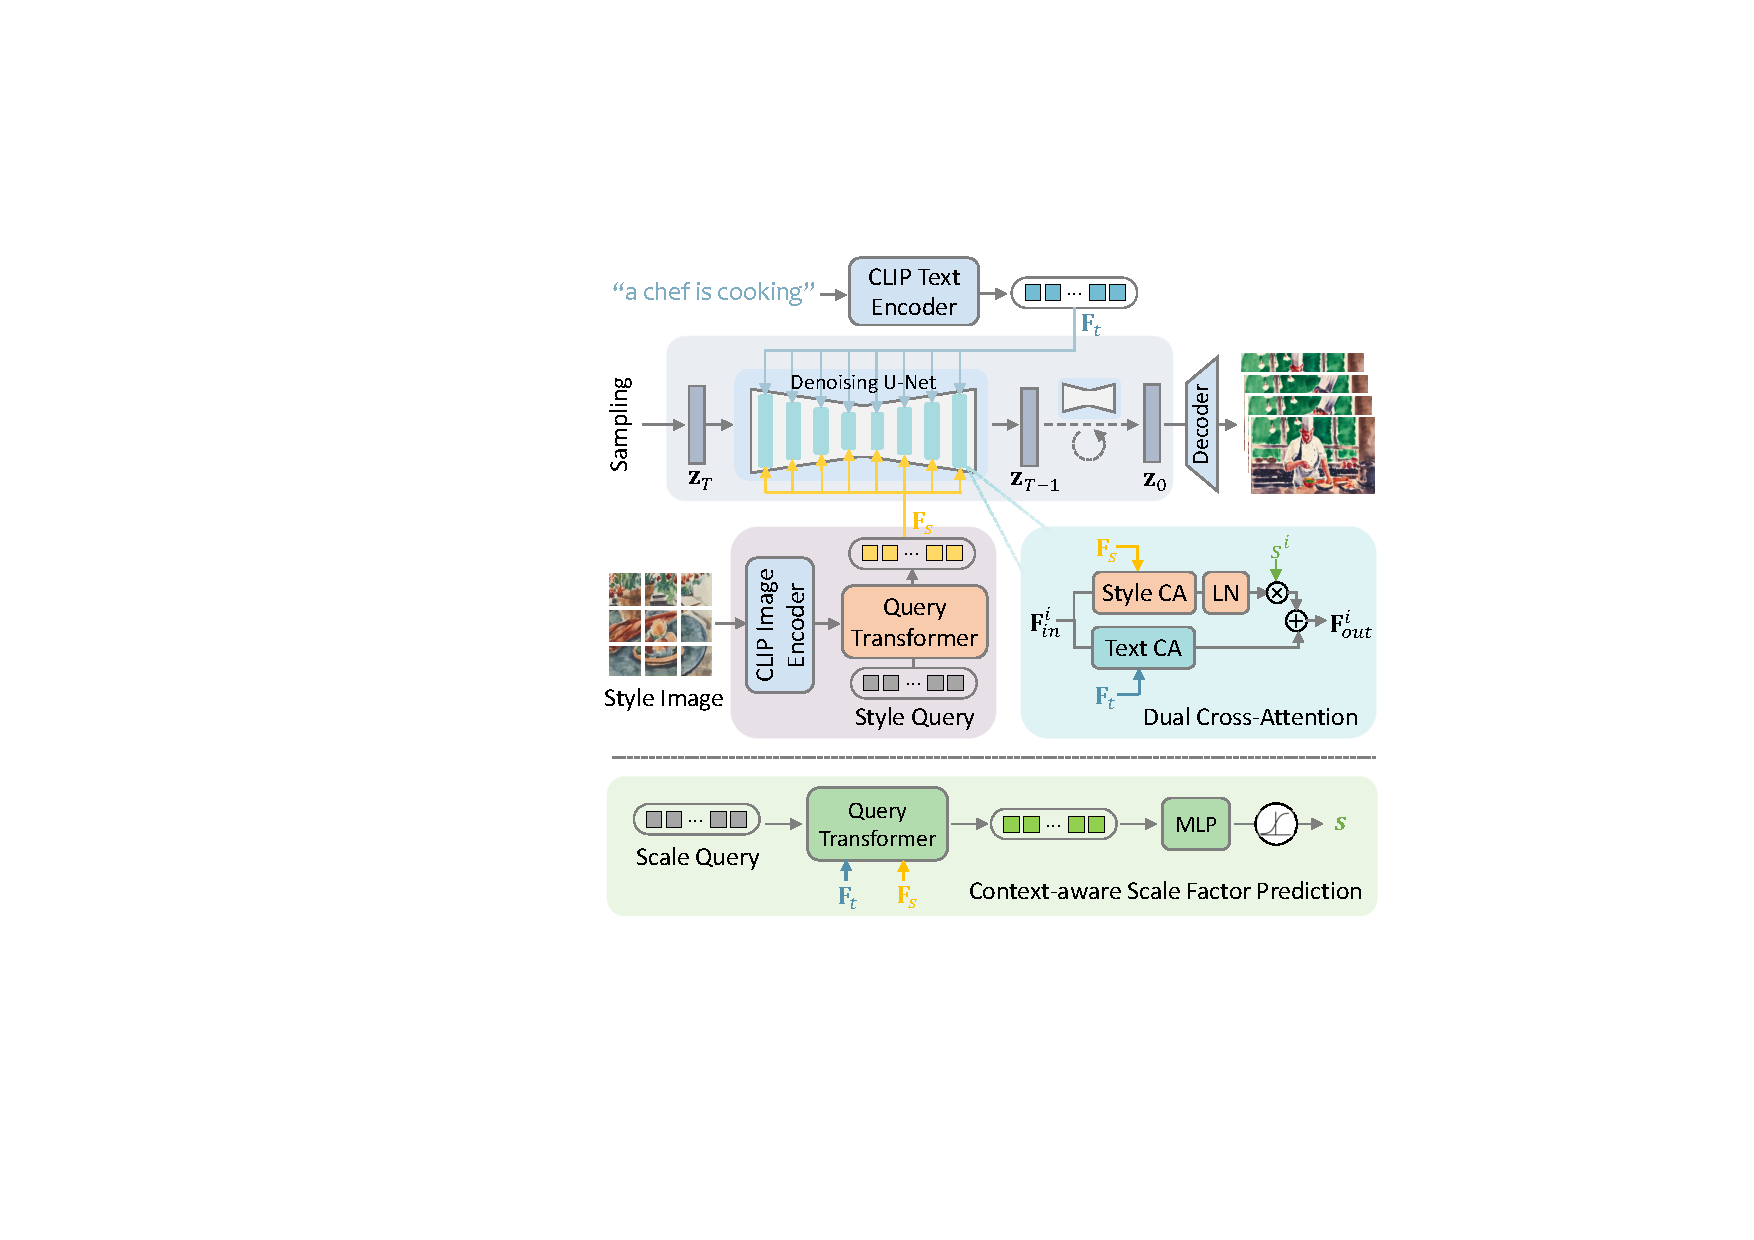
\includegraphics[width=0.95\linewidth]{figures/overview2.pdf}
    \vspace{-0.35cm}
    \caption{Overview of our proposed style adapter. It consists of three components, i.e. style feature extractor, dual cross-attention module, and context-aware scale factor predictor.}
    \label{fig:overview}
    \vspace{-1.4em}
\end{figure}


%---------------------------------
\vspace{-0.6em}
\subsection{Reference-Based Style Modulation}
\label{subsec:style_modulation}
%---------------------------------

Our style adapter serves to extract style features from the input reference image and infuse them into the backbone features of the denoising U-Net. As mainstream T2V models~\cite{chen2023videocrafter, chen2024videocrafter2, wang2023modelscope, wang2023lavie} are generally initialized from open-source T2I Models and trained with image and video datasets in a joint strategy, they support not only text-to-video generation but also retain the capacity for text-to-image generation. To overcome the scarcity of stylized videos, we propose to train the style adapter based on a pre-trained T2V model (i.e. VideoCrafter~\cite{chen2023videocrafter}) for stylized image generation under the supervision of stylistic images.

\vspace{-0.3em}
\paragraph{Content-Style Decoupled Data Augmentation.}
\label{sec:data_aug}
We use the stylistic images from two publicly available datasets, i.e. WikiArt~\cite{phillips2011wiki} and a subset of Laion-Aesthetics~\cite{schuhmann2022laion} (aesthetics score above 6.5). In the original image-caption pairs, we observe that the captions generally contain both content and style descriptions, and some of them do not match the image content well. To promote the content-style decoupling, we use BLIP\nobreakdash-2~\cite{li2023blip2} to regenerate captions for the images and remove certain forms of style description (e.g., \textit{a painting of}) with regular expressions.
In addition, as an image contains both style and content information, it is necessary to construct a decoupling supervision strategy to guarantee the extracted style feature free of content features. Although a stylistic image may contain different local style patterns~\cite{park2019arbitrary, huo2021manifold, chen2023tssat}, we regard that a large crop of an image(e.g. 50\% of the image) still preserves a similar style representation with the full image.
% We regard that every local regions of a stylistic image share the same style representation, which not only reflects on texture and color theme but also on the structure and perceptual semantics. 
Based on this insight, we process each stylistic image to obtain the target image and style image through different strategies: for target image, we scale the shorter side of the image to 512 and then crop the target content from the central area; for style image, we scale the shorter side of the image to 800 and randomly crop a local patch with $512 \times 512$. This approach reduces the overlap between the style reference and generation target, while still preserving the global style semantics complete and consistent.

\vspace{-0.3em}
\paragraph{Style Embedding Extraction.}
CLIP~\cite{radford2021learning} has demonstrated remarkable capability in extracting visual features from open-domain images. To capitalize on this advantage, we employ a pre-trained CLIP image encoder as a feature extractor. Specifically, we utilize both the global semantic token and the full $256$ local tokens (i.e., from the final layer of the Transformer) since our desired style embedding should not only serve as an accurate style trigger for the T2V model, but also provide auxiliary feature references.
As image tokens encompass both style and content information, we further employ a trainable Query Transformer (Q-Former)~\cite{li2023blip2} to extract style embedding $\mathbf{F}_s$. We create $N$ learnable style query embeddings as input for the Q-Former, which interact with image features through self-attention layers.
%We define style as the synthesized information present in an image that characterizes its overall aesthetic, independent of content. It encompasses both high-level aesthetic semantic information, such as composition, artistic conception, and color scheme, as well as low-level texture information, including specific brush stokes, lines, and surface details.
Note that this is a commonly adopted architecture for visual condition extraction~\cite{li2023blip2, shi2023instancebooth,ye2023ipadapter, xing2023dynamicrafter}. But it is the style-content fusion mechanism that makes our proposed design novel and insightful for style modulation, as detailed below.

\begin{figure}[t]
    \centering
    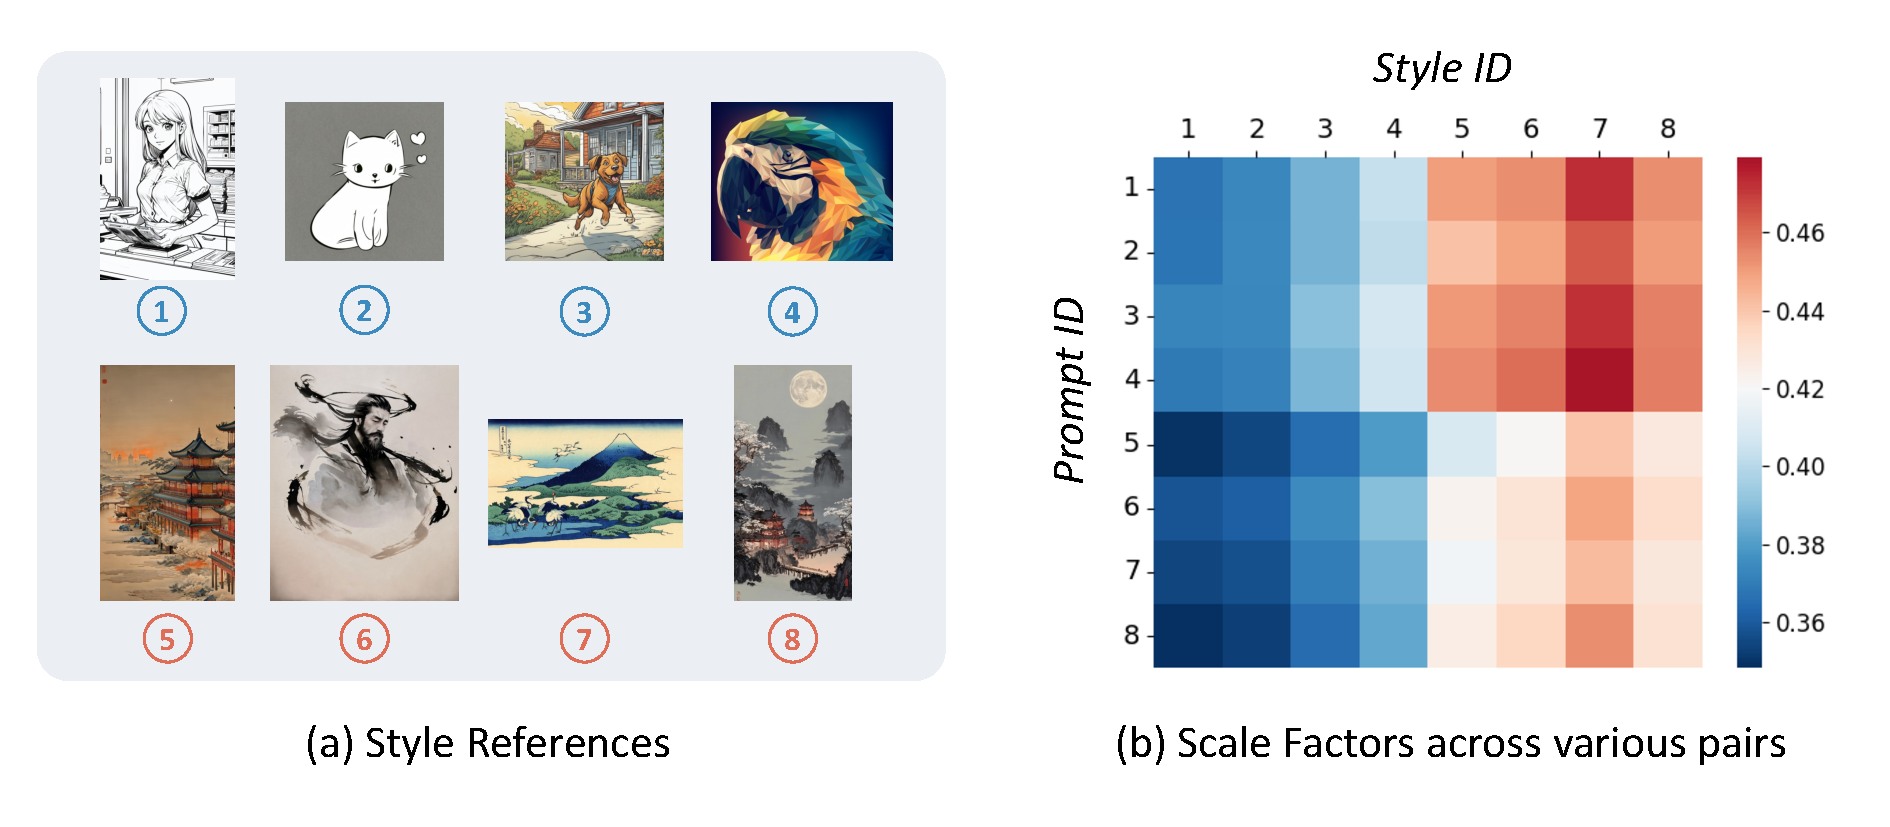
\includegraphics[width=\linewidth]{figures/scale_factor_viz.pdf}
    \vspace{-1.0cm}
    \caption{Illustration of content-style fusion scale factors across multiple input pairs. Four short prompts(less than 5 words) with prompt id $\in [1, 4]$ and four long prompts(more than 8 words) with prompt id $\in [5, 8]$ are randomly selected. Results indicate that shorter prompts and images with richer style-semantics tend to have relatively higher scale factors.} 
    \label{fig:scale_factor_viz}
    \vspace{-0.35cm}
\end{figure}

\paragraph{Adaptive Style-Content Fusion.}
\label{sec:fusion}
With the extracted style embedding, there are two ways to combine the style and text conditions, including (i) \textit{attach-to-text}~\cite{composer,gligen,ramesh2022hierarchical}: attach the style embedding to the text embedding and then interact with the backbone feature via the originally text-based cross-attention as a whole; (ii) \textit{dual cross-attention}~\cite{wei2023elite,ye2023ipadapter}: adding a new cross-attention module for the style embedding and then fuse the text-conditioned feature and style-conditioned feature.
According to our experiment (see Sec.~\ref{subsec:ablation}), solution (ii) surpasses solution (i) in disentangling the roles of text and style conditions, therefore we have adopted it as our final solution. The formula can be written as:
\vspace{-0.3em}
\begin{equation}
    \mathbf{F}_{out}^{i} = \text{TCA}(\mathbf{F}_{in}^i, \mathbf{F}_t) + s^i * \text{LN}(\text{SCA}(\mathbf{F}_{in}^i, \mathbf{F}_s)),
\end{equation}
where $\mathbf{F}_{in}^i$ denotes the backbone feature of layer $i$, LN denotes layer normalization, and TCA and SCA denote text-based cross attention and style-based cross attention respectively. $s^i$ is a scale factor learned by a context-aware scale factor prediction network, to balance the magnitudes of text-based feature and style-based feature.
The motivation is that different stylistic genres may have different emphasis on content expression. For example, the abstract styles tend to diminish the concreteness of the content, while realism styles tend to highlight the accuracy and specificity of the content. So, we propose a context-aware scale factor prediction network to predict fusion scale factors according to the input contexts.
Specifically, we create a learnable factor query, it interacts with textual features $\mathbf{F}_t$ and style features $\mathbf{F}_s$ to generate scale features via a Q-Former and then project it into layer-wise scale factors $\mathbf{s} \in \mathbb{R}^{16}$.
Figure~\ref{fig:scale_factor_viz} illustrates the learned scale factors across multiple contexts. It shows that the adaptive scale factors have a strong correlation with style genres while also depending on the text prompts. Style references with rich style-semantics(i.e., ukiyo-e style) typically yield higher scale factors to emphasize style; while complex prompts tend to produce lower scale factors to enhance content control.  This is consistent with our hypothesis to motivate our design.


%---------------------------------
\vspace{-0.5em}
\subsection{Temporal Adaptation to Stylized Features}
\label{subsec:temp_adaptation}
%---------------------------------

Given a pre-trained T2V model, the style adapter trained on image dataset works well for stylized image generation. However, it still struggles to generate satisfactory stylized videos, which is vulnerable to temporal jittering and visual artifacts.
The possible causes are that the cross-frame operations, i.e. temporal self-attention, do not involve in the process of stylized image generation, and thus induce incompatible issues. So, it is necessary to finetune the temporal self-attention with the style adapter incorporated.
Following the practice of T2V image and video joint training, the finetuning is performed on the mixed datasets of stylistic images and photorealistic videos. This is an adaptation training of temporal blocks while the other modules remain frozen, and the model converges efficiently.

\vspace{-0.5em}
\paragraph{Classifier-Free Guidance for Multiple Conditions.}
Unlike T2I models, video models exhibit a higher sensitivity to style guidance due to their limited stylized generation capabilities. Using a unified $\lambda$ for both style and context guidance may lead to undesirable generation results. Regarding this, we adopt a more flexible mechanism for multiple conditions classifier-free guidance. Building upon the vanilla text-guided classifier-free guidance, which controls context alignment by contrasting textual-conditioned distribution $\epsilon(z_t, c_t)$ with unconditional distribution $\epsilon(z_t, \varnothing)$, we introduce the style guidance with $\lambda_s$ by emphasizing the difference between the text-style-guided distribution $\epsilon(z_t, c_t, c_s)$ and the text-guided distribution $\epsilon(z_t, c_t)$. The complete formulation is as below:
\begin{equation}
    \begin{aligned}
        \hat{\epsilon}(z_t, c_t, c_s) = \epsilon(z_t, \varnothing) &+ \lambda_s(\epsilon(z_t, c_t, c_s) - \epsilon(z_t, c_t)) \\
        &+ \lambda_t(\epsilon(z_t, c_t) - \epsilon(z_t, \varnothing)),
    \end{aligned}
\end{equation}
where $c_t$ and $c_s$ denote textual and style condition respectively. $\varnothing$ denotes using no text or style conditions.
In our experiment, we follow the recommended configuration of text guidance in VideoCrafter~\cite{chen2023videocrafter}, setting $\lambda_t = 15.0$, while the style guidance is configured with $\lambda_s = 7.5$ empirically. Similarly, we set $\lambda_t = 7.5$ and $\lambda_s = 5.0$ for style-guided image generation.






% %---------------------------------
\vspace{-0.3em}
\section{Experimental Results}
\label{sec:result}
%---------------------------------

%---------------------------------
\subsection{Experimental settings}
\label{subsec:experiment_setting}
%---------------------------------

\paragraph{Implementation Details.} 
We adopt the VideoCrafter~\cite{chen2023videocrafter} as our base T2V model, which shares the same spatial weights with Stable Diffusion 2.1. We first train the style modulation on image dataset, i.e. WikiArt~\cite{phillips2011wiki} and Laion-Aesthetics-6.5+~\cite{schuhmann2022laion} for 40k steps with a batch size of 32 per GPU.  In the second stage, we froze the style modulation part and only train temporal blocks of VideoCrafter, we jointly train image datasets and video datasets(subset of WebVid-10M~\cite{bain2021frozen}) for 20k steps with a batch size of 1 on video data and 16 on image data, sampling image batches with a ratio of 20\%. The training process is performed on 8 A100 GPUs and can be completed within 3 days. Furthermore, to ensure a fair comparison with some SDXL-based models~\cite{ye2023ipadapter, hertz2023style} on stylized image generation, we also trained the first stage of StyleCrafter on SDXL~\cite{podell2023sdxl}. 
%The overall training process takes about 5 days on 8$\times$V100.

% We train the style adapter on xx for xx epoches, with xx frozen and only train xxxx. In the second stage, xxx. We use xx optimizer and learning rate of xxxx. Also, training dataset.  \TODO{complete this part}

\paragraph{Testing Datasets.}
\label{sec:test_dataset}
To evaluate the effectiveness and generalizability of our method, we construct testsets comprising content prompts and style references. For content prompts, we use GPT-4~\cite{openai2023gpt4v} to generate recognizable textual descriptions from four meta-categories~(human, animal, object, and landscape). We manually filter out low-quality prompts, retaining 20 image prompts and 12 video prompts. For style references, we collect 20 stylized images and 8 sets of style images with multi-reference~(each contains 5 to 7 images in similar styles) from the Internet. In total, the test set contains 400 pairs for stylized image generation, and 300 pairs for stylized video generation (240 single-reference pairs and 60 multi-reference pairs). Details are available in the supplementary materials.

% 1. Content Prompt(generated from GPT4)
% 2. Style Image(selected from internet)
% 3. Content Image(generated from SD, for some style transfer method)
% 4. Style Prompt(generated from GPT4-v, for sd and video-crafter)

\paragraph{Evaluation Metrics.}
\label{sec:eval_metrics}
Following previous practice~\cite{zhang2023inversion, sohn2023styledrop, wang2023styleadapter}, we employ CLIP-based~\cite{radford2021learning} scores and DINO-based~\cite{caron2021emerging} scores to measure the text alignment and style conformity. Following EvalCrafter~\cite{liu2023evalcrafter}, we measure the temporal consistency of video generation by (i) calculating clip scores between contiguous frames and (ii) calculating the warping error on every two frames with estimated optical flow. 
Note that these metrics are not perfect. For example, one can easily achieve a close-to-1 style score by entirely replicating the style reference. Similarly, stylized results may yield inferior text scores compared to realistic results, even though both accurately represent the content descriptions. We recommend a comprehensive consideration of both CLIP-based text scores and style scores, rather than relying solely on a single metric.

\paragraph{User Preference Study.}
In addition to quantitative analysis, we conducted a user study to make comparisons among our method, VideoCrafter, Gen-2, and AnimateDiff in the context of single-reference and multi-reference stylized video generation. Users are instructed to select their preferred option based on style conformity, temporal quality, and all options fulfill text alignment for each comparison pair. We randomly chose 15 single-reference pairs and 10 multi-reference pairs, collecting 1125 votes from 15 users. 
Further details can be found in the supplementary materials.

%
\begin{table*}[!t]
\centering
%\setlength{\tabcolsep}{3.0pt}
% \renewcommand\arraystretch{1.5}
\caption{Quantitative comparison on single-reference style-guided T2I generation. We conduct evaluation on a test set of 400 pairs. \textbf{Bold}: Best. }
\label{tab:img_quan_clip}
\vspace{-1em}
\resizebox{0.93\linewidth}{!}{
  \begin{tabular}{ccccccccc} % {@{}lc@{}}
    \toprule
     \multirow{2}{*}{Method} & \multicolumn{4}{c}{\textbf{Stable Diffusion 2.1 based}} & \multicolumn{4}{c}{\textbf{SDXL based}} \\
    \cmidrule(lr){2-5}\cmidrule(lr){6-9}
     & Dreambooth & InST & SD* & Ours & IP-Adapter-Plus & Style-Aligned & SDXL* & Ours(SDXL)  \\
    \midrule
    \texttt{CLIP-Text} $\uparrow$ & \textbf{0.3047}  & 0.3004 & 0.2766 & 0.3028 & 0.2768 & 0.2254 & 0.2835 & \textbf{0.2918} \\
    \texttt{CLIP-Style} $\uparrow$ & 0.3459 & 0.3708 & 0.4183 & \textbf{0.4836} & 0.5182 & 0.5515 & 0.4348 & \textbf{0.5615} \\
    \texttt{DINO-Style} $\uparrow$ & 0.2278 & 0.2587 & 0.2890 & \textbf{0.3652} & 0.4367 & 0.4395 & 0.2912 & \textbf{0.4514} \\
    \bottomrule
  \end{tabular}
}
\end{table*}



%---------------------------------
\subsection{Style-Guided Text-to-Image Generation}
\label{subsec:image_eval}
%---------------------------------

As mentioned in Sec.~\ref{subsec:style_modulation} and Sec.~\ref{subsec:experiment_setting}, our proposed method also supports to generate stylized images~(using model before temporal finetuning). We are interested to evaluate our method against state-of-the-art style-guided T2I synthesis methods, which are better-established than video counterparts. The competitors include optimization-based methods like DreamBooth~\cite{dreambooth}, inversion-based methods such as InST~\cite{zhang2023inversion} and Style-Aligned~\cite{hertz2023style}, and adapter-based methods like IP-Adapter-Plus~\cite{ye2023ipadapter}. Besides, we consider two unique competitors: SD*~\cite{ldm} and SDXL*~\cite{sdxl}~(text-to-image models equipped with GPT-4V~\cite{openai2023gpt4v}, where GPT-4V generates textual descriptions about the reference's style and merges them with content prompts as input for models). This comparison aims to validate the advantages of employing image conditions to enhance stylized generation instead of relying solely on text conditions.
Implementation details of competitors are available in supplementary materials.
% For each style, DreamBooth and CustomDiffusion are optimized with the provided single reference image to learn the customized concept of style.
%This setting may degrade their performance (because they usually requires 5~20 images to learn a concept) but it is fair comparison since all the methods are only provided with a single style image.

The quantitative comparison is tabulated in Table~\ref{tab:img_quan_clip}. 
% Although our method achieved the best performance on both metrics, we would like to emphasise that clip-based metrics are imperfect.As discussed in Sec.~\ref{sec:eval_metrics}, the CLIP-Text is measured by the similarity between content text embedding and stylized image embedding, the stylistic appearance actually hinders the metric in some extent, which makes those methods with weak stylistic effects (i.e. close to photorealism) achieve superior scores. 
Results reveal that Dreambooth~\cite{dreambooth} and InST~\cite{zhang2023inversion} struggle to accurately capture the style from various style references and exhibit low style conformity. SD*~\cite{ldm} and SDXL~\cite{sdxl} demonstrate good stylistic ability but still fail to reproduce the style of the reference image, possibly because of the text’s inherent clumsiness in expressing specific styles despite utilizing the powerful GPT4V for visual style understanding. IP-Adapter~\cite{ye2023ipadapter} and style-aligned~\cite{hertz2023style} generate aesthetically pleasing images, while their style-content decoupled learning is not perfect and exhibits limited control over content.
In contrast, our method efficiently generates high-quality stylized images that align with the content of the texts and resemble the style of the reference image. Our method demonstrates stable stylized generation capabilities when dealing with various types of prompts.


%---------------------------------
\subsection{Style-Guided Text-to-Video Generation}
\label{subsec:video_eval}
%---------------------------------

\begin{figure*}[t!]
    \centering
    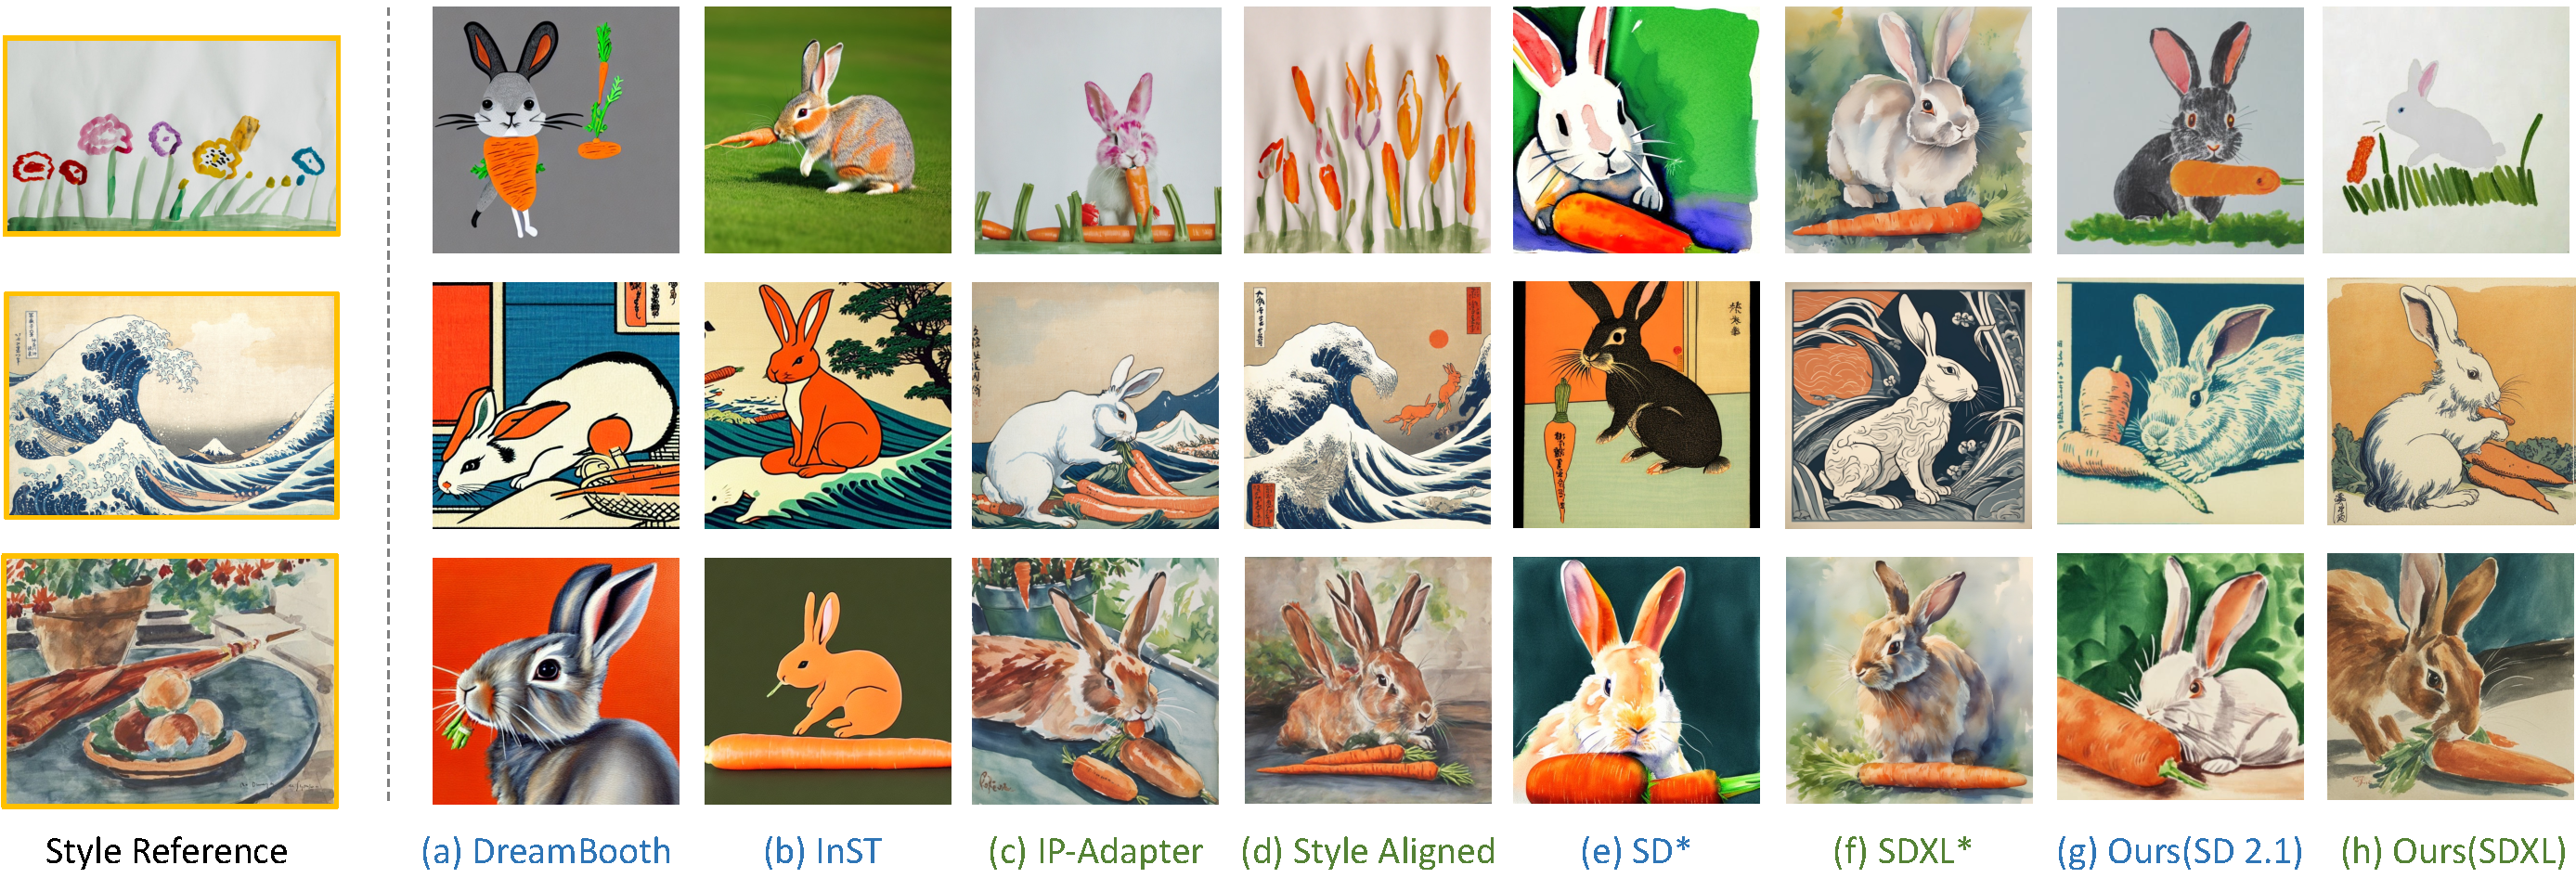
\includegraphics[width=0.87\linewidth]{figures/comp_image.pdf}
    \vspace{-1em}
    % \vspace{-2em}
    \caption{Visual comparison on style-guided T2I generation. \textcolor[RGB]{46, 117, 182}{Blue}: methods based on SD 2.1. \textcolor[RGB]{84, 130, 53}{Green}: based on SDXL. Prompt: A rabbit nibbling on a carrot.} 
    \label{fig:result_img}
    \vspace{-1em}
\end{figure*}
%
\begin{figure*}[!h]
    \centering
    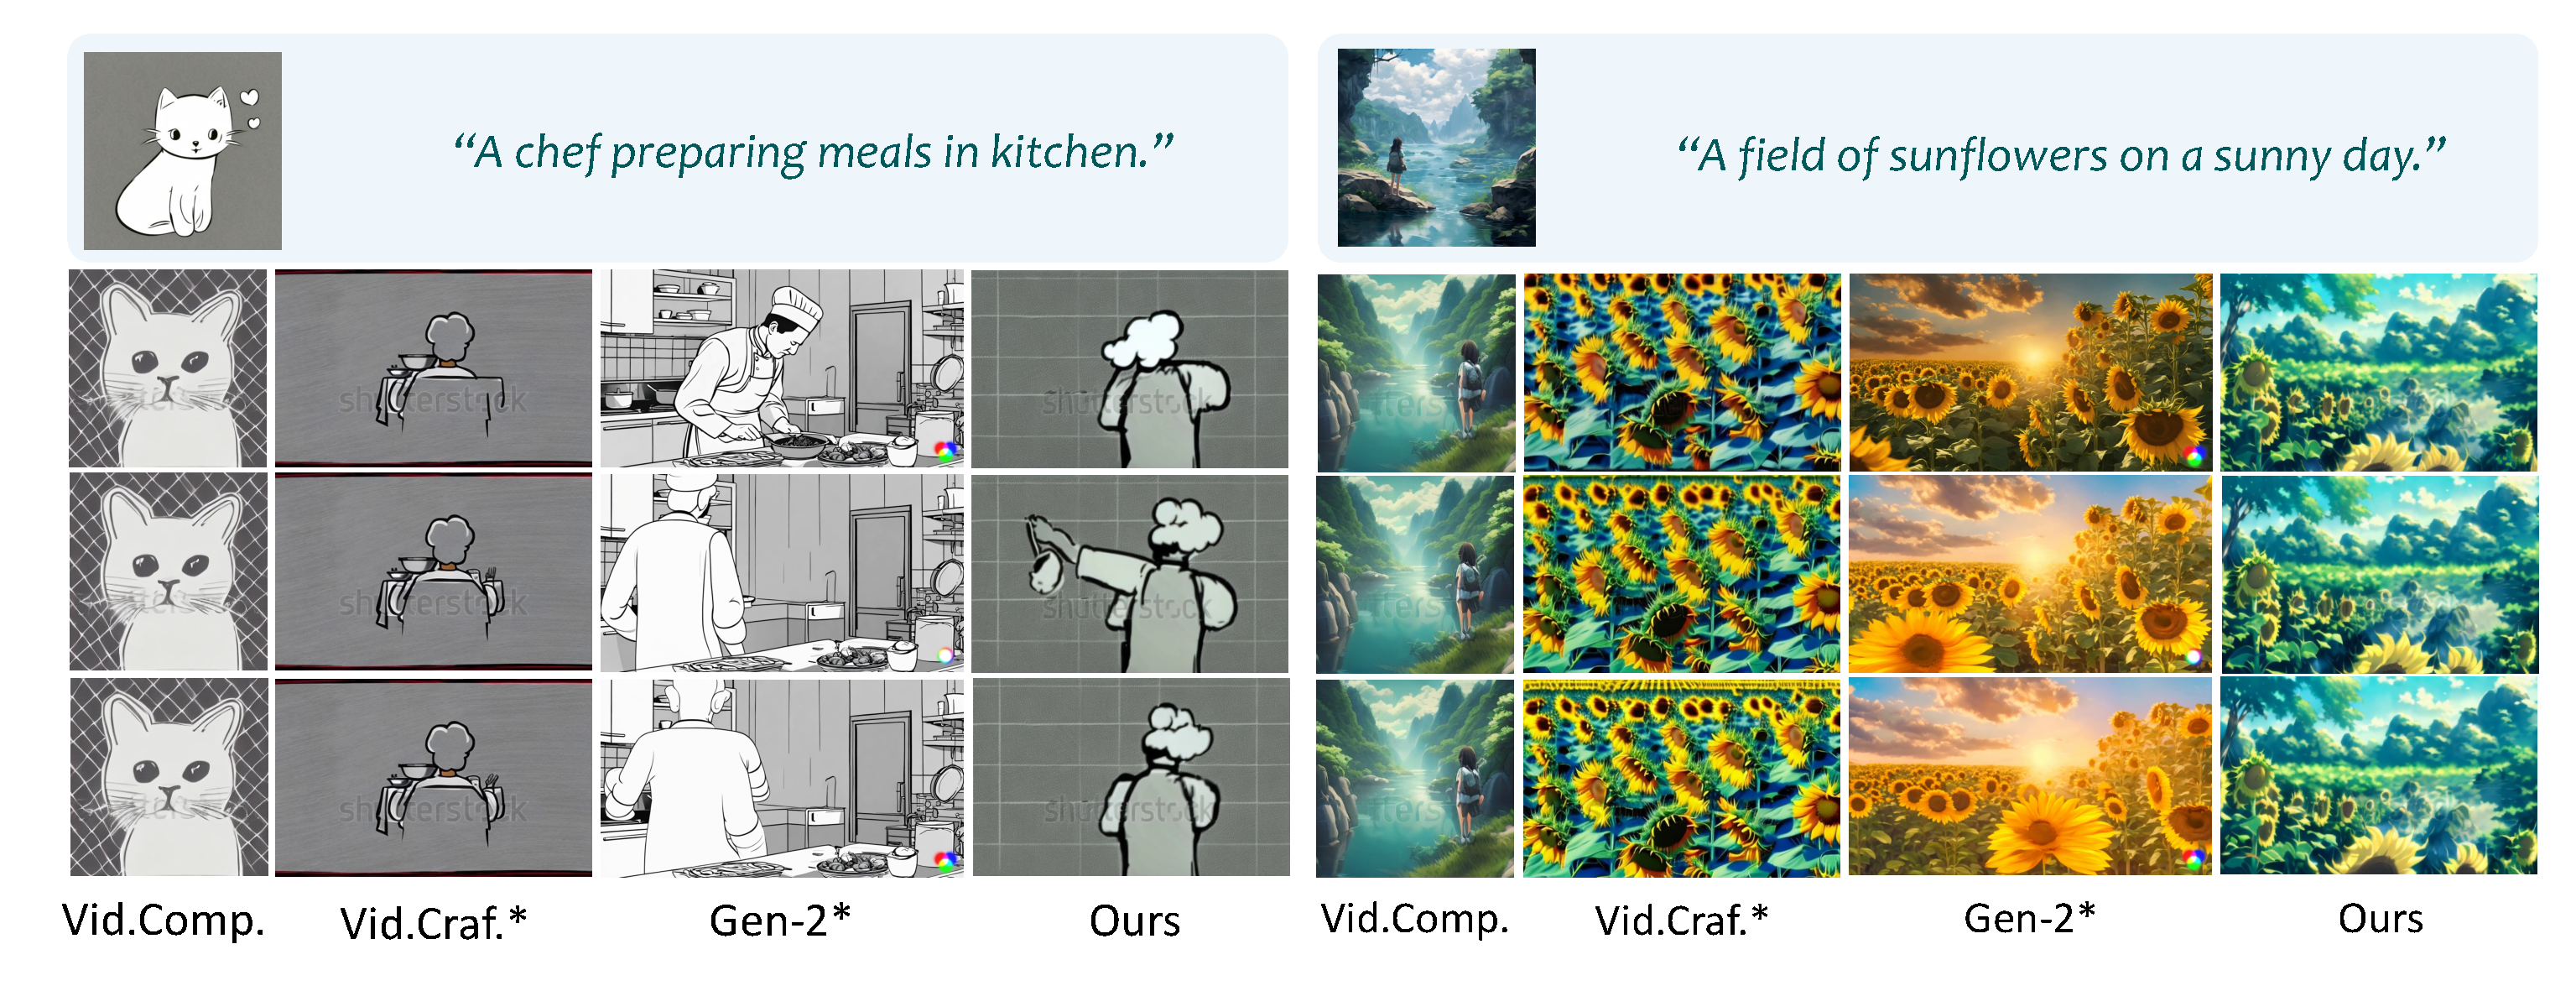
\includegraphics[width=0.9\linewidth]{figures/comp_video.pdf}\vspace{-1.5em}
    \caption{Visual comparison of single-reference guided T2V generation. Vid.Comp.: VideoComposer, Vid.Craf.: VideoCrafter
    %Our approach accurately captures the style of the reference image and generates videos that satisfy both text alignment and style conformity.
    } 
    \label{fig:result_video}
    \vspace{-1em}
\end{figure*}
%
\begin{figure*}[!h]
    \centering
    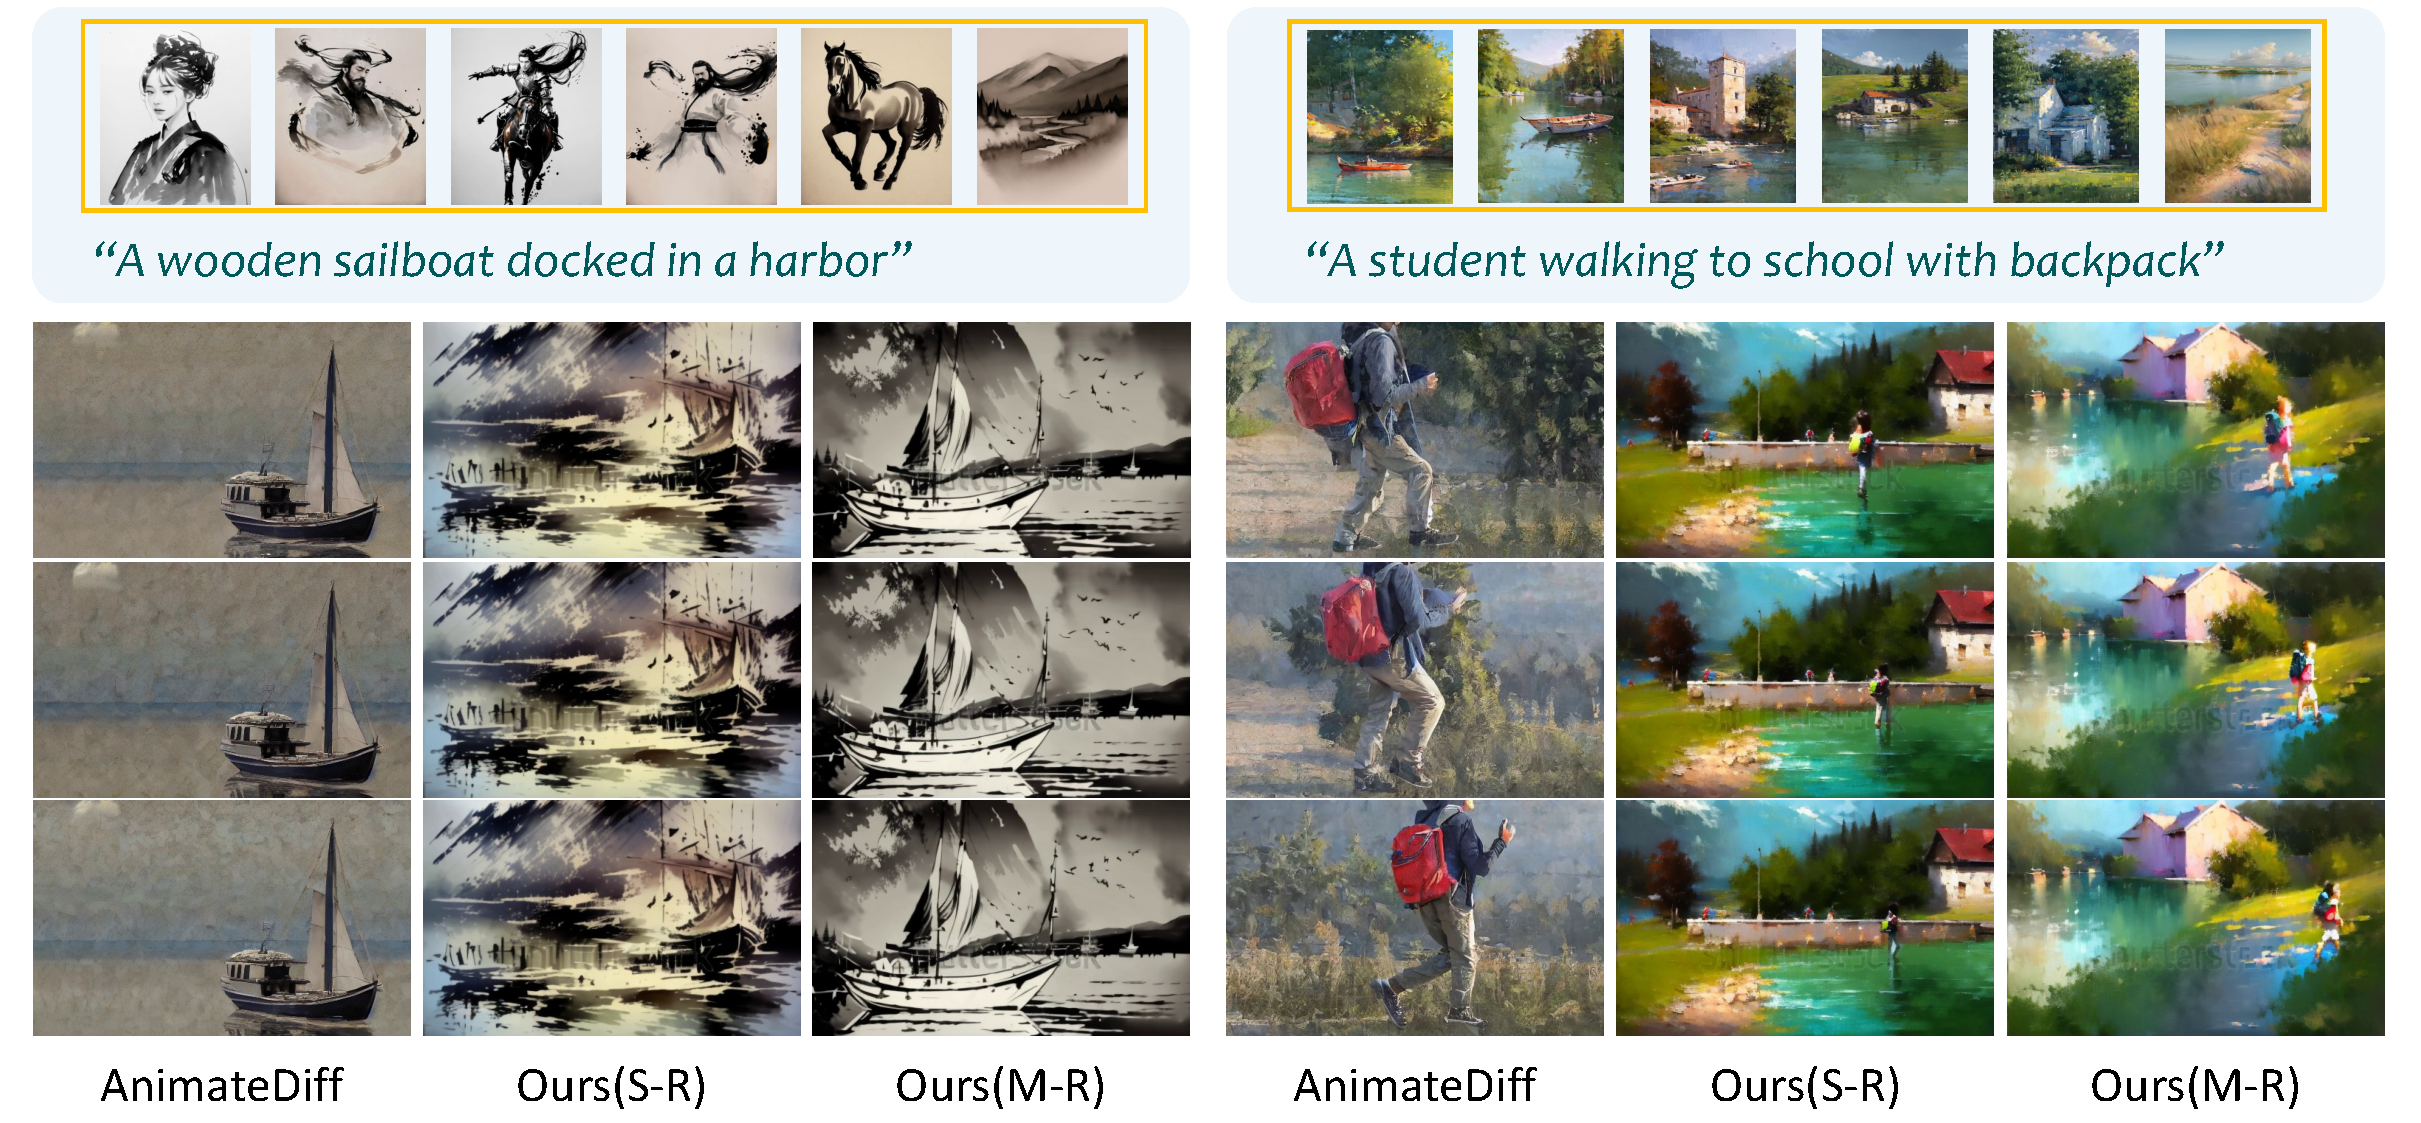
\includegraphics[width=0.87\linewidth]{figures/comp_video2.pdf}
    \vspace{-1em}
    \caption{Qualitative comparison of multi-reference style-guided T2V generation. S-R: Single-Reference, M-R: Multi-Reference
    %AnimateDiff tends to generate close-to-reamlism results despite the style references are typical artistic styles. In contrast, our approach performs better in text alignment, style conformity and temporal consistency.
    } 
    \vspace{-1em}
    \label{fig:result_multi_ref}
\end{figure*}



\begin{table}[!t]
\centering
\caption{Quantitative comparison of style-guided T2V generation. Top 3 rows: single-reference based gudiance. Bottom 3 rows: multi-reference based guidance. S-R: Single-Refernce, M-R: Multi-Reference, W.E.: Warping Errors.}
\label{tab:video_quan_clip}
\vspace{-1em}
\resizebox{\linewidth}{!}{
% \scriptsize
% \renewcommand\arraystretch{1.2}
\begin{tabular}{c c c cc} % {@{}lc@{}}
    % \toprule
    \toprule
    \multirow{2}{*}{Methods} & \multirow{2}{*}{CLIP-Text $\uparrow$} & \multirow{2}{*}{CLIP-Style $\uparrow$} & \multicolumn{2}{c}{Temporal Consistency} \\
    \cmidrule(lr){4-5}
      & & &
     ~CLIP-Temp $\uparrow$~ & \makecell{W.E.($\times10^{-3}$) $\downarrow$}\\
    \midrule
    VideoComposer & 0.0468 & \textbf{0.7306} & 0.9853 & \textbf{9.903} \\
    VideoCrafter* & 0.2209 & 0.3124 & 0.9757 & 61.41 \\
    Ours & \textbf{0.2726} & 0.4531 & \textbf{0.9892} & 18.73 \\
    \midrule
    ~AnimateDiff & \textbf{0.2867} & 0.3528 & 0.8903 & 37.17 \\
    Ours(S-R) & 0.2661 & 0.4803 & 0.9851 & 14.13 \\
    Ours(M-R) & 0.2634 & \textbf{0.4887} &\textbf{0.9852} & \textbf{9.396} \\
    \bottomrule
  \end{tabular}
}
\end{table}

\begin{table}[!t]
\centering

\caption{User study statistics of the selection rate for text alignment(\texttt{Text}), and preference rate for style conformity(\texttt{Style}) and temporal quality(\texttt{Temporal}). Top 3 rows: single-reference based guidance. Bottom 2 rows: multi-reference based guidance.}
\label{tab:video_quan_multi_ref}
\vspace{-1em}

\small
\begin{tabular}{c c c c} % {@{}lc@{}}
    % \toprule
    \toprule
    Methods & \texttt{Text} $\uparrow$ & \texttt{Style} $\uparrow$ & \texttt{Temporal} $\uparrow$ \\
    \midrule
    VideoCrafter* & 0.391 & 8.0\% & 4.4\%  \\
    Gen-2* & 0.747 & 23.1\% & 51.1\% \\
    Ours & 0.844 & 68.9\% & 44.4\% \\
    \midrule
    ~AnimateDiff~ & 0.647 & 10.0\% & 19.3\% \\
    Ours(M-R) & 0.907 & 90.0\% & 80.7\% \\
    \bottomrule
\end{tabular}
\end{table}

Existing approaches for style-guided video generation can be divided into two categories: one is the single-reference based methods that are usually tuning-free, e.g. VideoComposer~\cite{wang2024videocomposer}; the other is the multi-reference based methods that generally requires multiple references for fine-tuning, e.g. AnimateDiff~\cite{guo2023animatediff}. We make comparisons with these methods, respectively. 
% Apart from the quality metrics, we further conduct user study to evaluate the stylized video results, including text alignment, style conformity and temporal quality.


\vspace{-0.5em}
\paragraph{Single-Reference based Guidance.}VideoComposer~\cite{wang2024videocomposer} is a controllable video generation model that allows multiple conditional inputs including style reference image. It is a natural competitor of our method. 
Besides, we construct two additional comparative methods, i.e. VideoCrafter* and Gen2*, which extend VideoCrafter~\cite{chen2023videocrafter} and Gen2~\cite{Gen-2}, the state-of-the-art T2V models in open-source and close-source channels respectively, to make use of style reference images by utilizing GPT-4V~\cite{openai2023gpt4v} to generate style prompts from them.
% The evaluation is conducted on 240 text-style pairs, as introduced in Sec.~\ref{sec:test_dataset}. 
The quantitative comparison is tabulated in Table~\ref{tab:video_quan_clip}. Several typical visual examples are illustrated in Figure~\ref{fig:result_video}.

We can observe that: 
(i) VideoComposer tends to copy content from style references and struggles to generate text-aligned content, which is possibly because of the invalid decoupling learning. Consequently, its results exhibit abnormally high style conformity and very low text alignment. In addition, VideoComposer often generates static videos, thus having the lowest warping errors, but this does not mean that their results perform best in temporal quality. 
(ii) VideoCrafter* exhibits limited stylized generation capabilities, producing videos with diminished style and disjointed movements. Gen-2* demonstrates superior stylized generation capabilities. However, Gen-2 is still limited by the inadequate representation of style in textual descriptions, and is more prone to sudden changes in color and luminance. (iii) In comparison, our method captures styles more effectively and reproduces them in the generated results.

\begin{figure}[!t]
    \centering
    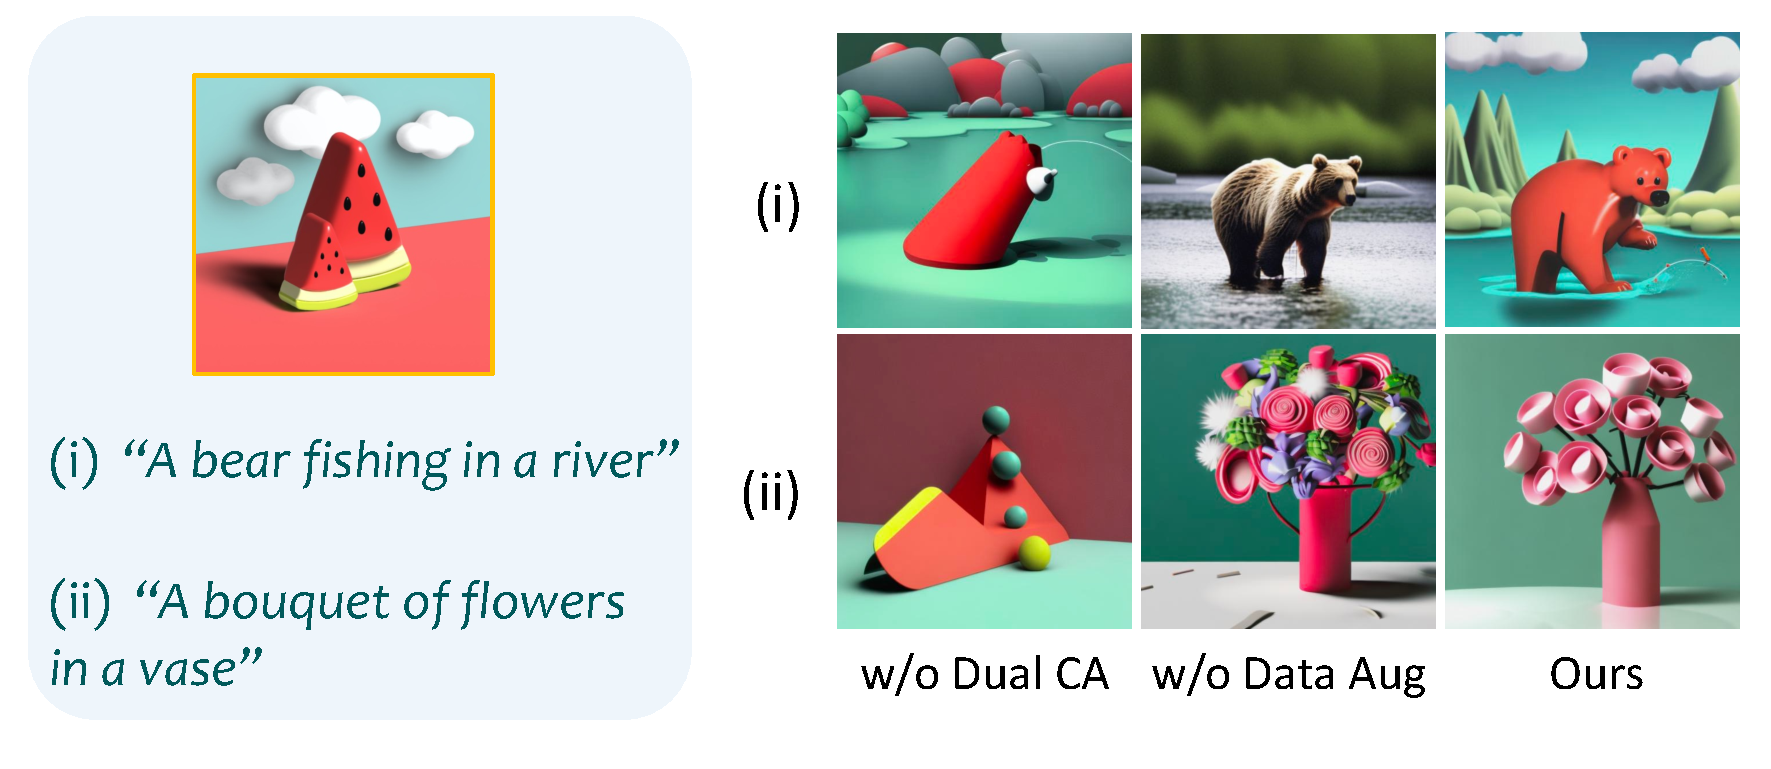
\includegraphics[width=\linewidth]{figures/ablation_img_1.pdf}
    \vspace{-3em}
    \caption{Effects of dual cross-attention and data augmentation.} 
    \label{fig:ablation_img_1_2}
    \vspace{-1em}
\end{figure}


\vspace{-0.5em}
\paragraph{Multi-Reference based Guidance.}
AnimateDiff~\cite{guo2023animatediff} denotes a paradigm to turn personalized SD (i.e., SD fine-tuned on specific-domain images via LoRA~\cite{hu2022lora} or Dreambooth~\cite{dreambooth}) for video generation, namely combined with pre-trained temporal blocks of T2V models. It can generate very impressive results if the personalized SD is carefully prepared, however, we find it struggle to achieve as satisfactory results if only a handful of style reference images are available for training.
We conduct an evaluation on 60 text-style pairs with multi-references, as presented in Sec.~\ref{sec:test_dataset}. We train Dreambooth~\cite{dreambooth} models for each style and incorporate them into AnimateDiff based on their released codebase. Thanks to the flexibility of Q-Former, our method also supports multiple reference images in a tuning-free fashion, i.e. computing the image embeddings of each reference image and concatenating all embeddings as input to the Q-Former.
Results are compared in Table~\ref{tab:video_quan_multi_ref} and Figure~\ref{fig:result_multi_ref} respectively.

According to the results, AnimateDiff struggles to achieve high-fidelity stylistic appearance while tends to generate close-to-realism results despite the style references are typical artistic styles. In addition, it is vulnerable to temporal artifacts. As the trained personalized-SD can generate decent stylistic images (provided in the supplementary materials), we conjecture that the performance degradation is caused by the incompatibility from the pre-trained temporal blocks and independently trained personalized-SD models, which not only interrupts temporal consistency but also weakens the stylistic effect.
In contrast, our method can generate temporal consistent videos with high style conformity to the reference images and accurate content alignment with the text prompts. Furthermore, using multiple references can further promote the performance, which offers additional advantages in practical applications.


%---------------------------------
\subsection{Ablation Study}
\label{subsec:ablation}
%---------------------------------

\begin{figure}[!t]
    \centering
    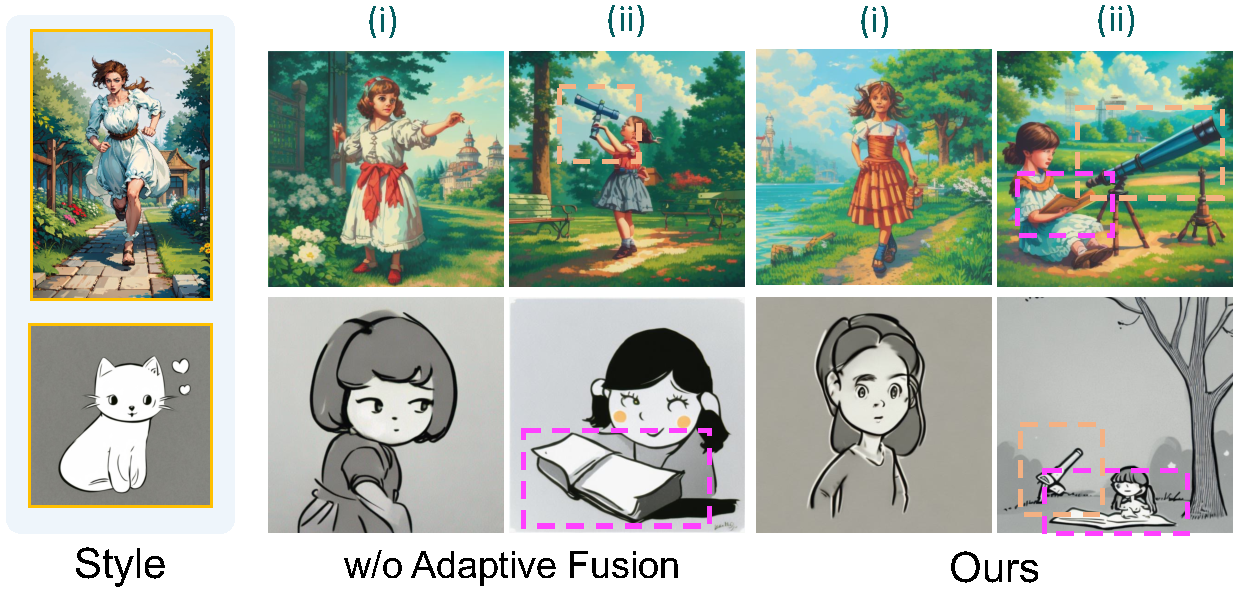
\includegraphics[width=\linewidth]{figures/ablation_no_scale.pdf
    }
    \vspace{-2em}
    \caption{Effect of adaptive content-style fusion. It shows superiority in generalization to extreme cases, e.g. long text description. Two text prompts are used: (i) A little girl; (ii) \textit{A little girl \textcolor[RGB]{255, 64, 255}{reading a book} in the park, with \textcolor[RGB]{244, 177, 131}{a telescope} nearby pointed at the sky}.}
    \label{fig:ablation_no_fusion}
    \vspace{-0.7em}
\end{figure}

% We make ablation studies on some important designs of our method, including data augmentation, module architectures, and training strategies, to validate their effectiveness.

\paragraph{Data Augmentation.}
We first study the effectiveness of content-style decoupled data augmentation. As depicted in Table~\ref{tab:ablation_img}, training with the original image-caption pairs restricts the model's ability to extract style representations, leading to lower style conformity. For example, as shown in Figure~\ref{fig:ablation_img_1_2}, method without data augmentation fails to capture the "3D render" style from the reference.


\paragraph{Dual Cross-Attention.} 
As discussed in Sec.~\ref{subsec:style_modulation},  we make a comparison between \textit{attach-to-text} and \textbf{dual cross-attention} to study their effects. Results are presented in Table ~\ref{tab:ablation_img} and Figure~\ref{fig:ablation_img_1_2}, revealing that \textit{attach-to-text} tends to directly fuse the content from the reference image and the text prompts rather than combining the text-based content and image-based style. This indicates the effectiveness of \textbf{dual cross-attention} in facilitating content-style decoupling.


\paragraph{Adaptive Style-Content Fusion.}
As previously discussed in Figure~\ref{fig:scale_factor_viz}, our proposed adaptive style-content fusion module demonstrates effectiveness in adaptively processing various conditional contexts. It benefits the generalization ability of model to deal with diverse combinations of content prompt and style image. Figure~\ref{fig:ablation_no_fusion} reveals that although the baseline can handle easy prompt inputs like "A little girl", it struggles to accurately generate all objects described in longer prompts. In contrast, the adaptive fusion module can achieve decent text alignment for long text descriptions thanks to its flexibility to adaptive balance between content and style.

\paragraph{Two-Stage Training Scheme.}
Our proposed training scheme consists of two stages, i.e., style adapter training and temporal adaption. To show its necessity, we build two baselines: (i) \textit{w/o Temporal Adaption}: that we train a style adapter on image data and apply it directly to stylized video generation without finetuning; (ii) \textit{joint training}: that we conduct style adapter training and temporal blocks finetuning on image-video dataset simultaneously.
As depicted in Table~\ref{tab:ablation_video}, baseline (i) exhibits inferior temporal consistency when applied directly to video, and undermines the content alignment and style conformity. As for baseline (ii), the learning of style embedding extraction seems to be interfered by the joint finetuning of temporal blocks, which impedes it to generate desirable stylized videos.


\begin{table}[!t]
\centering

\caption{Ablation studies on style modulation designs. The performance is evaluated based on the style-guided T2I generation.}
\label{tab:ablation_img}
\vspace{-1em}
    
\small
% \renewcommand\arraystretch{1.2}
  \begin{tabular}{ccc} % {@{}lc@{}}
    % \toprule
    \hline
    Methods & \texttt{CLIP-Text} $\uparrow$ & \texttt{CLIP-Style} $\uparrow$ \\
    \hline
    Ours & 0.3028 & 0.4836 \\
    ~w/o Data Augmentation & 0.3173 & 0.4005 \\
    w/o Dual Cross Attention & 0.0983 & 0.7332 \\
    w/o Adaptive Fusion & 0.2807 & 0.4925 \\
    \hline
  \end{tabular}
\vspace{-1em}
\end{table}


\begin{table}[!t]
\centering
\vspace{1em}

\caption{Ablation study on our two-stage training scheme.}
\vspace{-1em}
\label{tab:ablation_video}
% \renewcommand\arraystretch{1.5}
\resizebox{\linewidth}{!}{

\begin{tabular}{c c c cc} % {@{}lc@{}}
    % \toprule
    \toprule
    \multirow{2}{*}{Methods} & \multirow{2}{*}{CLIP-Text $\uparrow$} & \multirow{2}{*}{CLIP-Style $\uparrow$} & \multicolumn{2}{c}{Temporal Consistency} \\
    \cmidrule(lr){4-5}
      & & &
     ~CLIP-Temp $\uparrow$~ & \makecell{W.E.($\times10^{-3}$) $\downarrow$}\\
    \midrule
    w/o Temporal Adaption  & 0.2691 & 0.3923 & 0.9612 & 47.88 \\
    Joint Training & 0.3138 & 0.2226 & 0.9741 & 24.74 \\
    Two-Stage(ours) & \textbf{0.2726} & \textbf{0.4531} & \textbf{0.9892} & \textbf{18.73} \\
    \bottomrule
  \end{tabular}
}

    \vspace{-1em}
  
\end{table}

%
% \begin{figure}[!t]
%     \centering
%     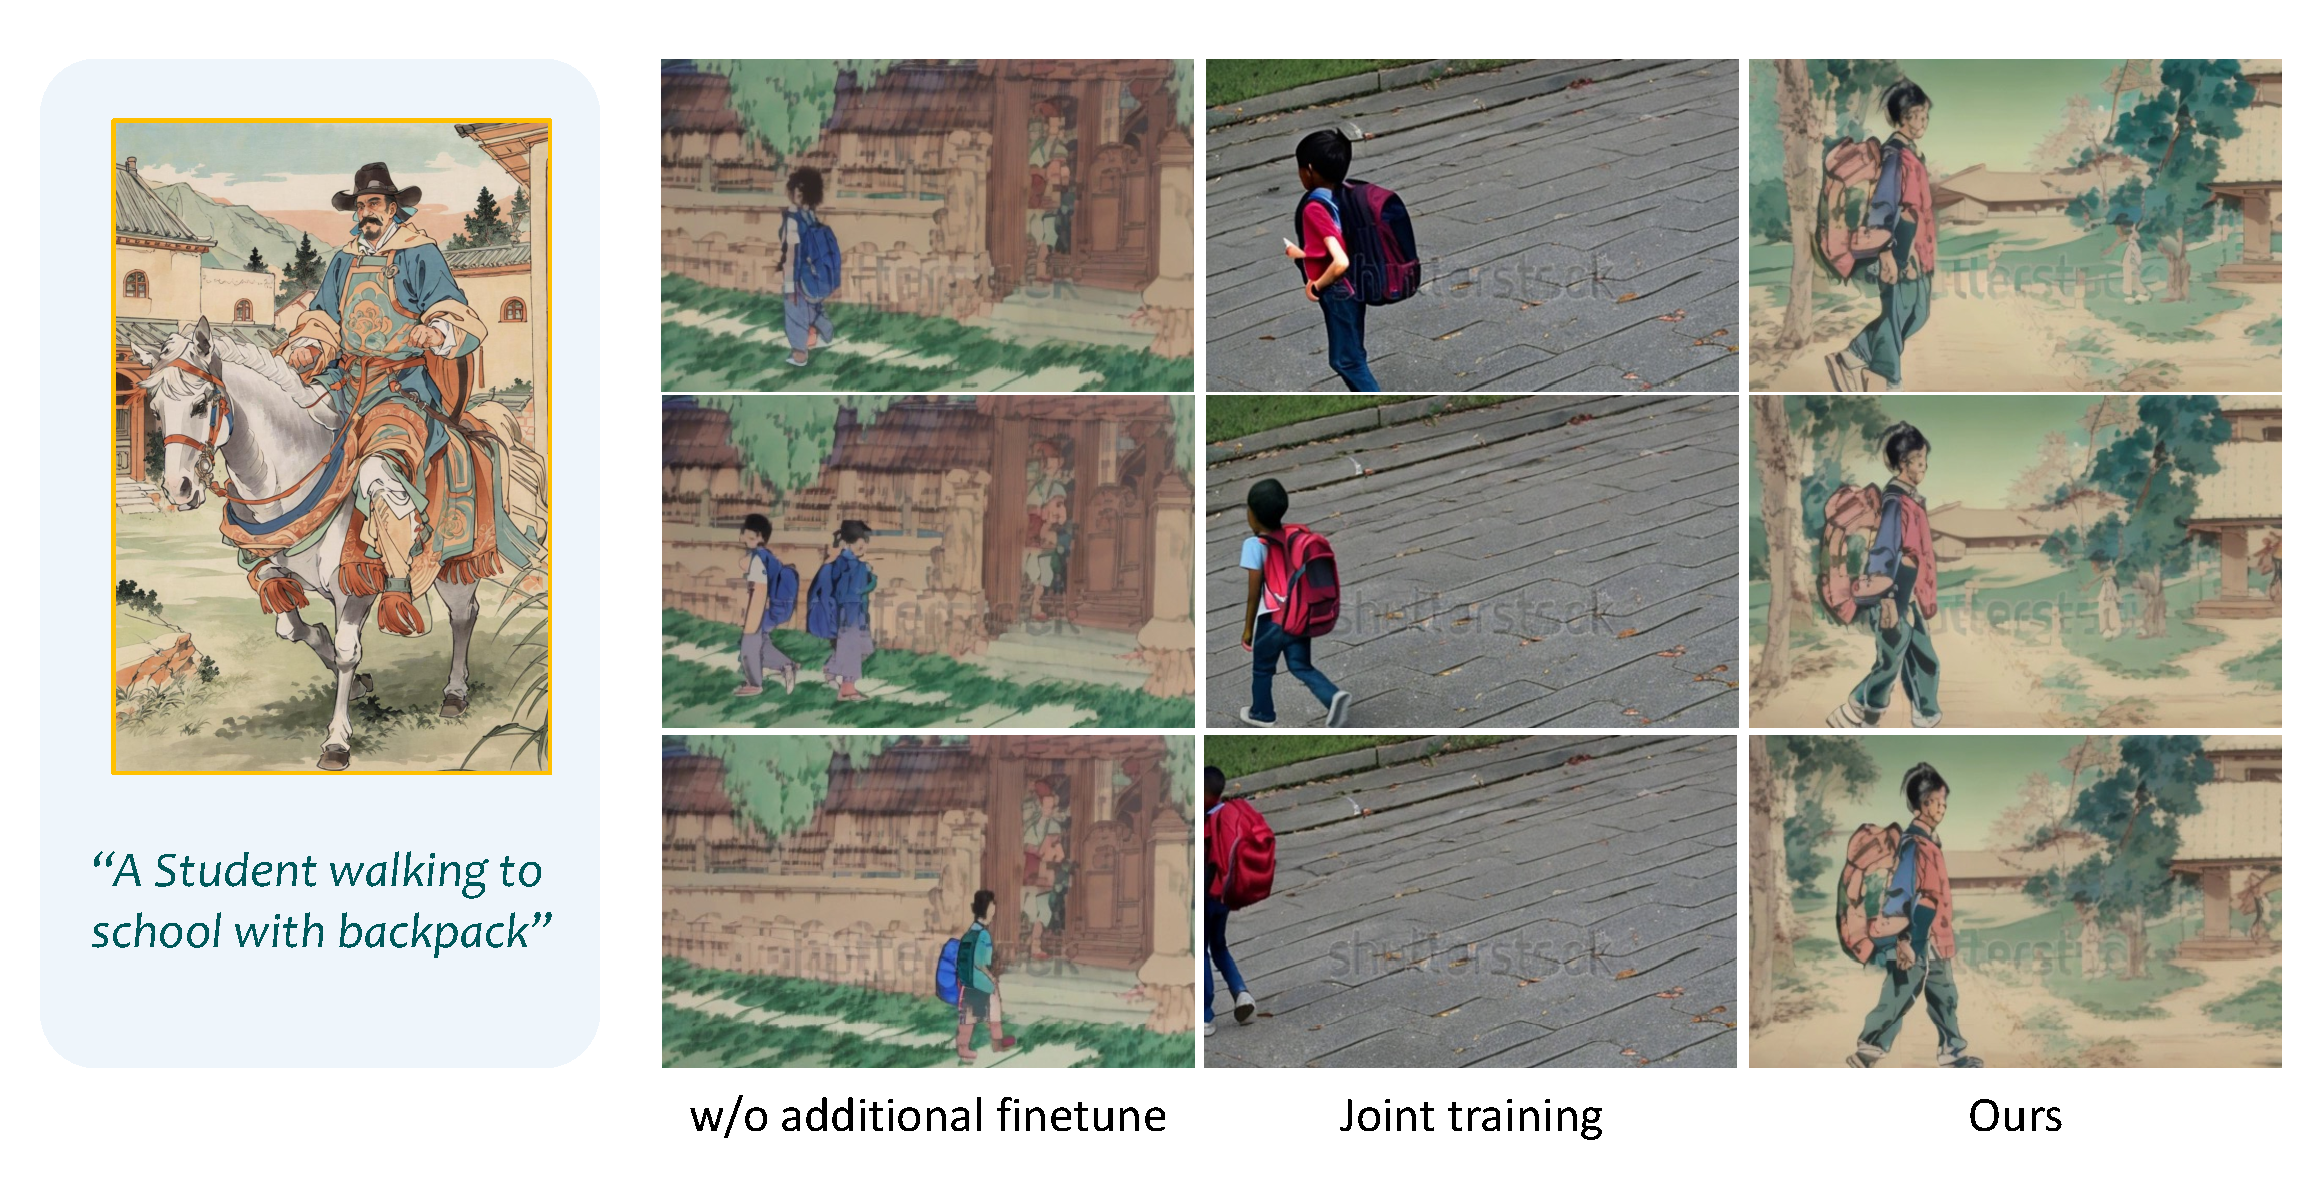
\includegraphics[width=\linewidth]{figures/ablation_two_stage.pdf}
%     \vspace{-2em}
%     \caption{Comparison on the effects of different training schemes.}
%     \label{fig:ablation_two_stage}
%     \vspace{-1em}
% \end{figure}



% \section{Conclusion}

We have explored the direct application of Transformers to image recognition.
Unlike prior works using self-attention in computer vision, we do not introduce image-specific inductive biases into the architecture apart from the initial patch extraction step.
Instead, we interpret an image as a sequence of patches and process it by a standard Transformer encoder as used in NLP.
This simple, yet scalable, strategy works surprisingly well when coupled with pre-training on large datasets.
Thus, \oursfull matches or exceeds the state of the art on many image classification datasets, whilst being relatively cheap to pre-train.

While these initial results are encouraging, many challenges remain.
One is to apply \oursabbrv to other computer vision tasks, such as detection and segmentation.
Our results, coupled with those in \citet{carion20-detr}, indicate the promise of this approach.
Another challenge is to continue exploring self-supervised pre-training methods.
Our initial experiments show improvement from self-supervised pre-training, but there is still large gap between self-supervised and large-scale supervised pre-training.
Finally, further scaling of \oursabbrv{} would likely lead to improved performance.

% \citestyle{acmauthoryear}
% \bibliographystyle{ACM-Reference-Format}
% \bibliography{reference}
% \end{bibunit}

% \begin{bibunit}
% \clearpage
% 
\newpage
\appendix
\section*{Appendix}
In support of the main paper,~\cref{app:proofs} presents the proofs for the propositions in the paper,~\cref{app:additional_findings} includes additional findings that support our main results, and~\cref{app:further_discussion} provides further discussion on conditions that lead to grokking.
\section{Proofs}\label{app:proofs}
\begin{proof}[Proof of~\cref{prop:stablemax}]
\begin{align}
    \softmax\left(g\left(x_i\right)\right) &= \frac{e^{g(x_i)}}{\sum_j e^{g(x_j)}}\\
    &= \begin{cases}
\frac{e^{\log(x_i+1)}}{\sum_j e^{\log(x_j+1)}} & \text{if } x_i \geq 0, \\
\frac{e^{-\log(-x_i+1)}}{\sum_j e^{-\log(-x_j+1)}} & \text{if } x_i < 0
\end{cases}\\
&= \begin{cases}
\frac{x_i+1}{\sum_j x_j+1} & \text{if } x_i \geq 0, \\
\frac{\frac{1}{-x_i+1}}{\sum_j \frac{1}{-x_j+1}} & \text{if } x_i < 0
\end{cases}\\
&= \stablemax(x_i).
\end{align}
\end{proof}

\begin{proof}[Proof of~\cref{prop:NLMGrad}]
To prove that any nonzero $-\nabla_{\perp} \loss(\bm{\theta}_t)$ is a descent direction, we need to show that $\left\langle -\nabla_{\perp} \loss(\bm{\theta}_t), \nabla\loss(\bm{\theta}_t) \right\rangle < 0$, assuming $\nabla_{\perp} \loss(\bm{\theta}_t) \neq \mathbf{0}$:
    \begin{equation}
        \left\langle \nabla\loss(\bm{\theta}_t), -\nabla\loss(\bm{\theta}_t) + \left( \frac{\bm{\theta}_t^\top \nabla \loss(\bm{\theta}_t)}{\bm{\theta}_t^\top \bm{\theta}_t} \right)\bm{\theta}_t  \right\rangle \leq 0.
    \end{equation}
    Expanding this yields:
    \begin{align}
        -\left\|\nabla\loss(\bm{\theta}_t)\right\|^2_2 + 
        \left\langle  \nabla\loss(\bm{\theta}_t), \bm{\theta}_t \frac{\bm{\theta}_t^\top \nabla \loss(\bm{\theta}_t)}{\bm{\theta}_t^\top \bm{\theta}_t}\right\rangle
        &\leq 0.
    \end{align}
    Since the inequality is unaffected by the scaling of the left hand side, we can, without loss of generality, assume that the gradients are normalized, leading to:
    \begin{align}\label{eq:incidence}
        \left\langle \nabla\loss(\bm{\theta}_t), \bm{\theta}_t \frac{\bm{\theta}_t^\top \nabla \loss(\bm{\theta}_t)}{\bm{\theta}_t^\top \bm{\theta}_t}\right\rangle
        &{\leq} 1.
    \end{align}
    Since $\bm{\theta}_t \frac{\bm{\theta}_t^\top \nabla \loss(\bm{\theta}_t)}{\bm{\theta}_t^\top \bm{\theta}_t}$ denotes the projection of the gradient onto the space spanned by the weights, $\langle\cdot,\cdot\rangle$ will measure the acute angle of incidence and hence~\cref{eq:incidence} holds, with equality iff $\nabla_{\perp} \loss(\bm{\theta}_t) = \mathbf{0}$, which is prevented by assumption. This proves that $-\nabla_{\perp} \loss(\bm{\theta}_t)$ is a descent direction while being perpendicular to the weights. %, the angle between $\loss(\bm{\theta}_t)$ and this projection will be the acute .
\end{proof}
We note that the \ograd stops when $\nabla_{\perp}\loss(\bm{\theta}_t) = \mathbf{0}$. If $\nabla\loss(\bm{\theta}_t) \neq \mathbf{0}$, this corresponds to the condition where the gradient is in the same direction with the parameter vector. $\nabla_{\perp}\loss(\bm{\theta}_t) = \mathbf{0}$ can also be the case if $\nabla\loss(\bm{\theta}_t) = \mathbf{0}$, which corresponds to the loss function being at a local optimum.

\section{Additional Findings}\label{app:additional_findings}


\subsection{Further evidence that SC prevents grokking} \label{app:sc_intervention}
\begin{wrapfigure}[12]{R}{0.38\textwidth}
            \vspace{-0.4cm}
            \begin{center}
    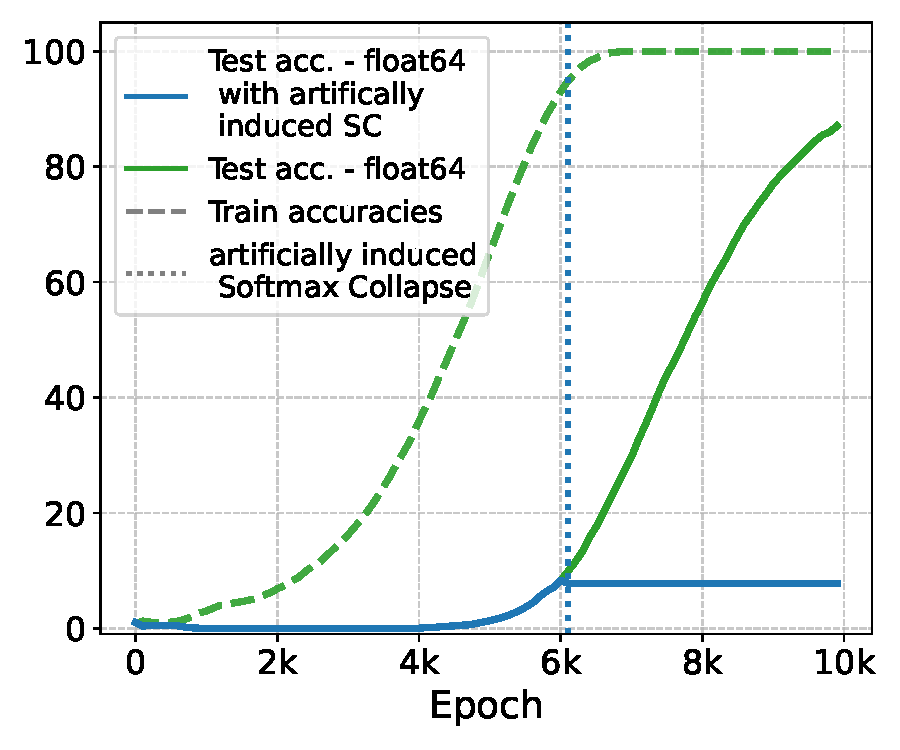
\includegraphics[width=\linewidth]{grokking_iclr_arxiv/figures/artificially_induced_sc.pdf}
            \end{center}
            \vspace{-12pt}
            \caption{Taking a model that would normally generalize (green) and artificially inducing SC has a very similar effect to the one observed in \cref{fig:grokking_stops}.\vspace{4mm}}
    \label{fig:sc_intervention}
\end{wrapfigure} 
While SC leads the gradient from correctly predicted samples to be zero, it does not do this for the incorrect classes. To validate that setting the gradients from the correct classes to zero is enough to stop learning, we do this artificially for a model that is generalizing and show that learning stops after this intervention. In \cref{fig:sc_intervention} we see that the baseline model shown in geen generalizes, but this is stopped at epoch 6000 for the model shown in blue, after we perform this intervention.

The intervention is implemented by multiplying the logits for the right classes by 0 at each step after epoch 6000.

\begin{comment}
\begin{figure}[h]
    \centering
    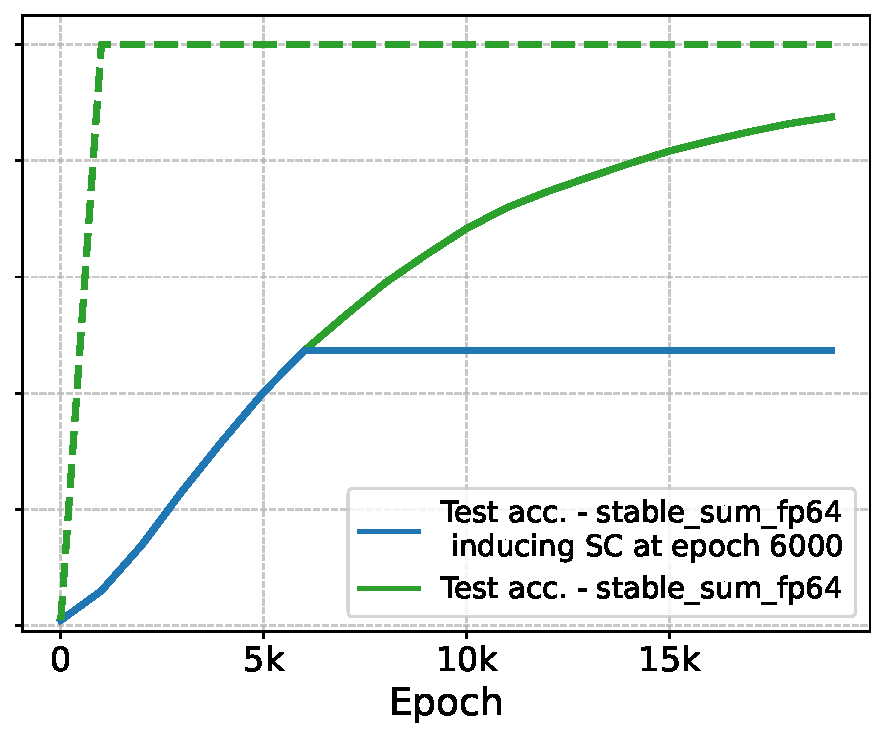
\includegraphics[width=0.5\linewidth]{grokking_iclr/figures/sc_intervention.pdf}
    \caption{Taking a model that would normally generalize (green) and artificially inducing SC has a very similar effect to the one observed in \cref{fig:grokking_stops}}.
    \label{fig:sc_intervention}
\end{figure}    
\end{comment}


\subsection{SGD with learning rate scheduling}
To show that our results are not due to the inductive bias of adaptive moments in optimizers like AdamW, we replicate some of the AdamW results using SGD with a learning rate scheduler. Our scheduler is similar to the one in \cite{Lyu2019-sc} except at each step we divide the learning rate by the norm of the full gradient, instead of the loss. In \cref{fig:grokking_stops_lr_sch} we observe that SC also puts an end to grokking in this setting.
\vspace{5.75mm}\\

\begin{figure}[t]
\centering
\begin{subfigure}{.32\textwidth}
  \centering
  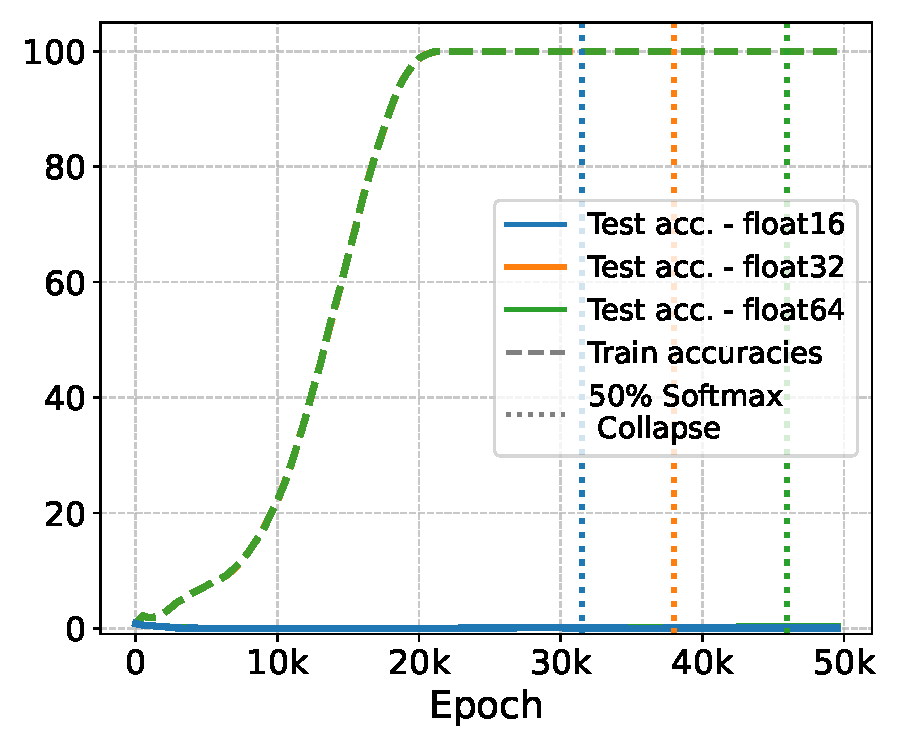
\includegraphics[width=\linewidth]{grokking_iclr_arxiv/figures/float32vsfloat64_40_percent_lr_sch.pdf}
  \caption{40\% training data}
  \label{fig:grokking_stops_40_lr_sch}
\end{subfigure}
\hfill
\begin{subfigure}{.32\textwidth}
  \centering
  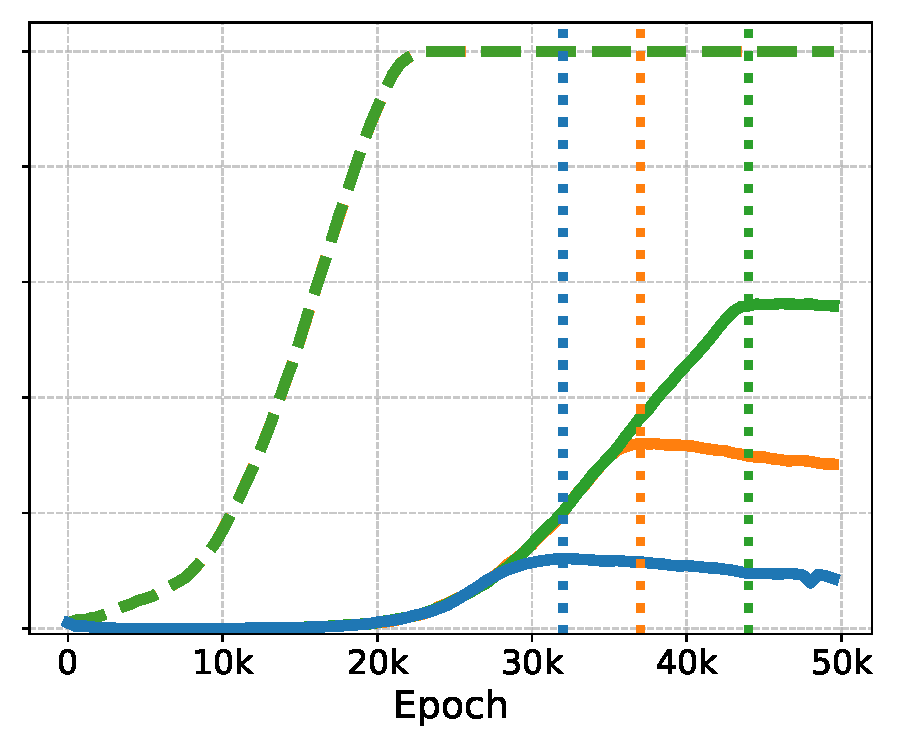
\includegraphics[width=\linewidth]{grokking_iclr_arxiv/figures/float32vsfloat64_60_percent_lr_sch.pdf}
  \caption{60\% training data}
  \label{fig:grokking_stops_60_lr_sch}
\end{subfigure}
\hfill
\begin{subfigure}{.32\textwidth}
  \centering
  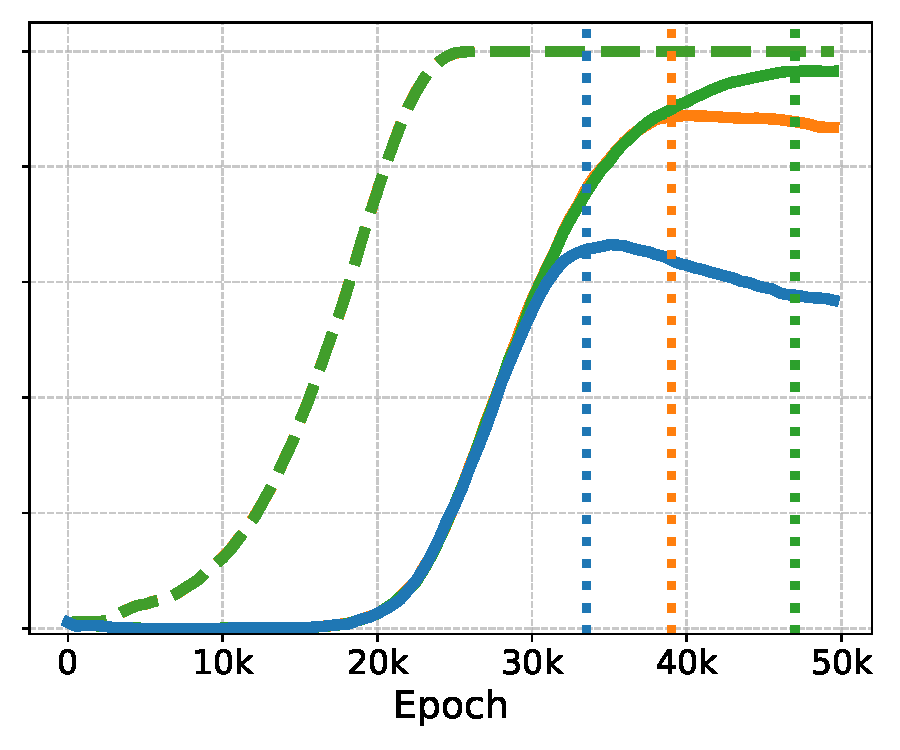
\includegraphics[width=\linewidth]{grokking_iclr_arxiv/figures/float32vsfloat64_70_percent_lr_sch.pdf}
  \caption{70\% training data}
\end{subfigure}
\caption{We show that the same dynamics observed in \cref{fig:grokking_stops} can be observed with a learning rate scheduler instead of AdamW. This shows that this is not due to an implicit bias of adaptive optimizers.}
\label{fig:grokking_stops_lr_sch}
\vspace{-5mm}
\end{figure}

\vspace{-5mm}
\section{Effective Learning Rate}
\begin{wrapfigure}[13]{R}{0.4\textwidth}
            \vspace{-1.2cm}
            \begin{center}
    \includegraphics[width=0.4\textwidth]{grokking_iclr_arxiv/figures/gradient_norms.pdf}
            \end{center}
            \vspace{-10pt}
            \caption{Gradient absorption errors during training on addition modulo 113.}
            \label{fig:gradient_absorption}
\end{wrapfigure} 
Unexplored in the main paper, NLM also has the effect of reducing the effective learning rate. For a gradient update using regular gradient descent $\bm{\theta}_{t+1} = \bm{\theta}_t - \eta \nabla \loss(\bm{\theta}_t)$ it is easy to see that $||\bm{\theta}_{t+1} - \bm{\theta}_{t}|| \to 0$ as $||\nabla \loss(\bm{\theta}_t)|| \to 0$. This problem has been observed before when training beyond the point of overfitting, for example, \cite{Lyu2019-sc} addressed it by using a loss based learning rate scheduler to keep up with the gradient. Theoretically, an alternative could be to simply extend the duration of training. According to our hypothesis, training for long enough should eventually lead to generalization on grokking tasks if we prevent SC. However, we find that another kind of floating point error can also appears in these settings, namely, gradient absorption errors in the weights. 

For a weight $w$, gradient absorption errors happen when a gradient update is small enough that it leaves the weight unchanged. Using the notation outlined in this paper this can be formalised as $w -\eta \frac{\partial \mathcal{L}}{\partial w} \doteq w$. In \cref{fig:gradient_absorption} we show that this happens for an MLP trained with SGD on modular addition using 30\% of the training data. As the norm of the gradient decreases, the percenage of the gradients that are absorbed by the weights increases substantially. Note that the number of gradients that are \textit{exactly} zero remains stable while the number of absorbed gradients increases substantially.

\begin{comment}
\begin{figure}[h]
    \centering
    \includegraphics[width=0.5\linewidth]{grokking_iclr/figures/gradient_norms.pdf}
    \caption{Gradient absorption errors during training on addition modulo 113.}
    \label{fig:gradient_absorption}
\end{figure}
\end{comment}
This issue is naturally mitigated by second order moments for adaptive optimizers like Adam and AdamW which is why they do not frequently appear. However, they do prevent us from showing grokking with vanilla gradient descent without any learning rate schduling. 


\subsection{Additional ways to induce grokking}
Beyond the interventions described in the main text, we highlight two additional ways to induce grokking that validate our hypothesis. 

\paragraph{Logit norm regularization}
Since we argue that uncontrolled scaling of the logits is responsible for delaying grokking and leading to SC, we validate that preventing this scaling of the logits by adding the norm of the logits to the loss, leads to grokking without additional regularization (\cref{fig:additional_grokking_logit}).


\begin{figure}[t]
\centering
\begin{subfigure}{.33\textwidth}
  \centering
  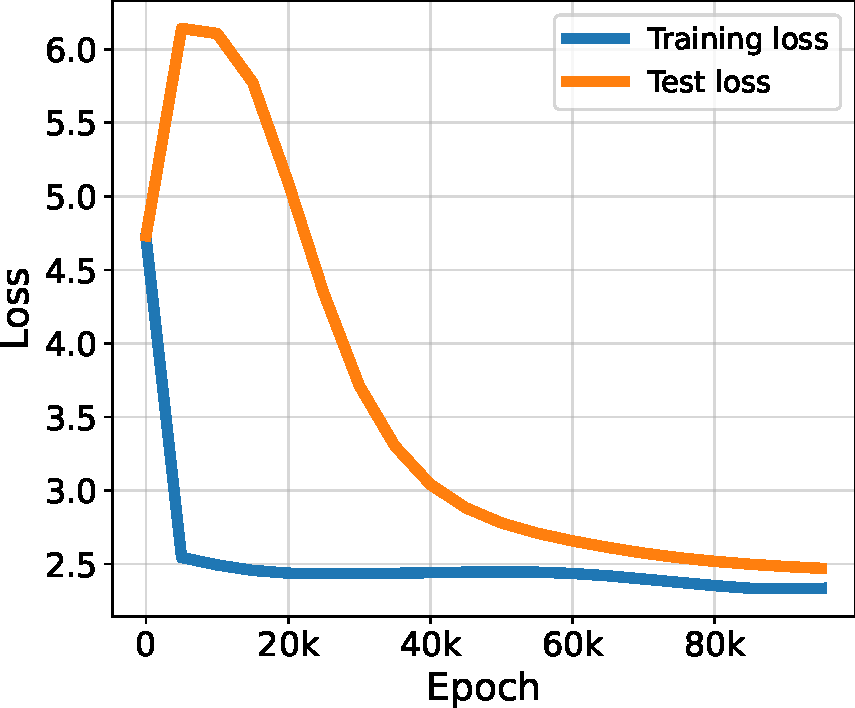
\includegraphics[width=\linewidth]{grokking_iclr_arxiv/figures/softermax_loss.pdf}
  \caption{$\stablemax$}
  \label{fig:additional_grokking_stablemax}
\end{subfigure}%
\hfill
\begin{subfigure}{.33\textwidth}
  \centering
  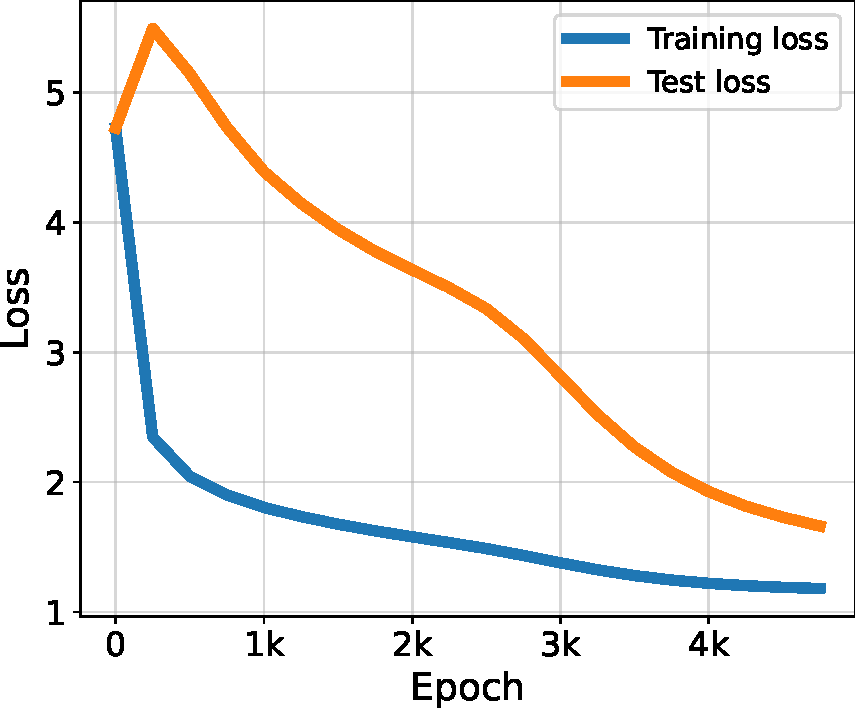
\includegraphics[width=\linewidth]{grokking_iclr_arxiv/figures/logit_reg_loss.pdf}
  \caption{Logit regularization}
  \label{fig:additional_grokking_logit}
  
\end{subfigure}%
\hfill
\begin{subfigure}{.33\textwidth}
  \centering
  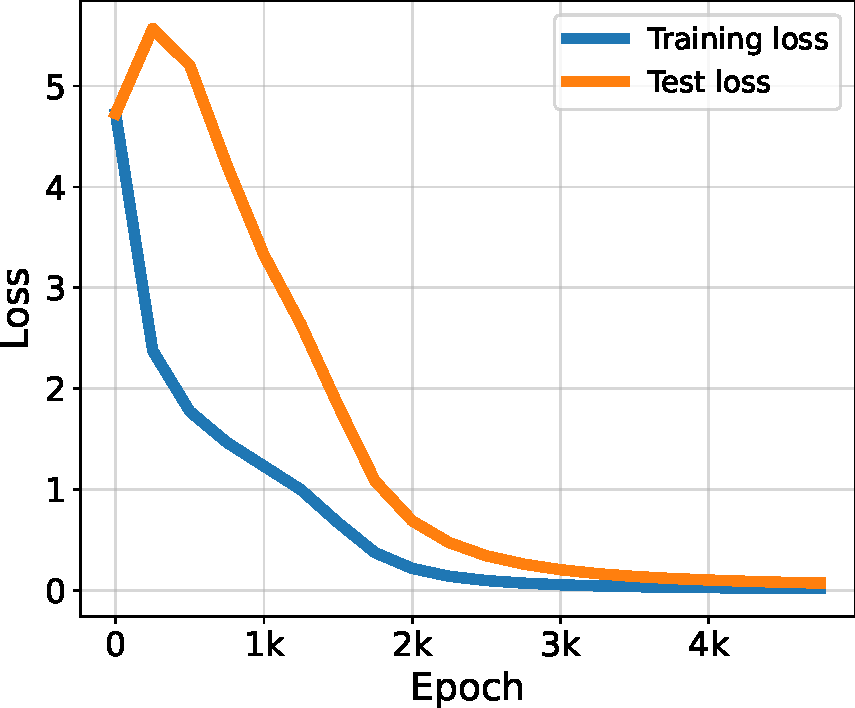
\includegraphics[width=\linewidth]{grokking_iclr_arxiv/figures/taylor_loss.pdf}
  \caption{\tsoftmax}
  \label{fig:additional_grokking_taylor}
\end{subfigure}
\vspace{-3mm}
\caption{Train and test losses during grokking induced by three different interventions.\vspace{-2mm}}
\label{fig:additional_grokking}
\end{figure}

\begin{wrapfigure}[20]{R}{0.4\textwidth}
\vspace{-0.5cm}
    \centering
    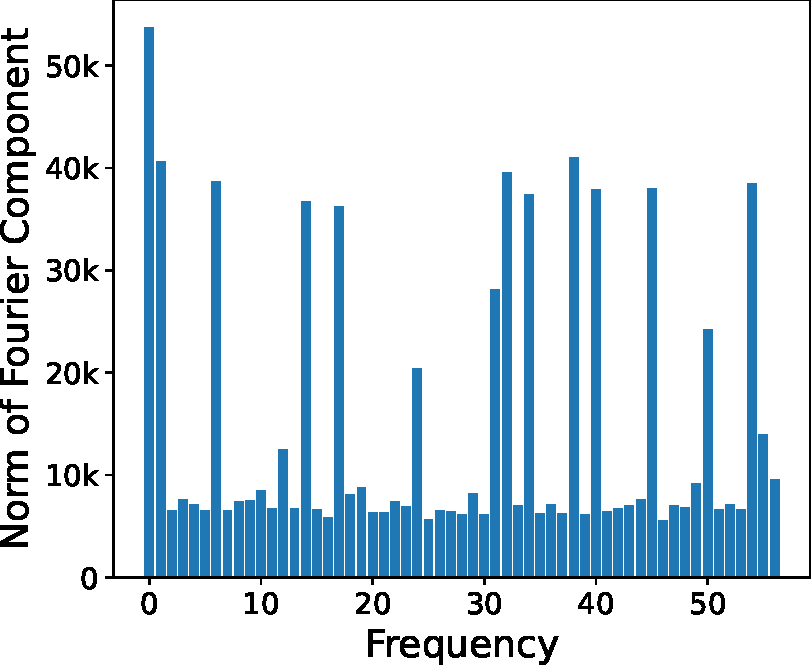
\includegraphics[width=\linewidth]{grokking_iclr_arxiv/figures/fourier.pdf}
    \vspace{-6mm}
    \caption{Fourier components of the weights of the output layer of an MLP trained on addition mod 113. Grokking is induced via $\stablemax$ and without weight decay.}
    \label{fig:fourier}
\end{wrapfigure}
\noindent\textbf{Taylor approximation of the Softmax.}
We have introduced $\stablemax$ as a change to the \softmax that leads to grokking without regularization. The motivation behind this is to prevent values in the sum of the \softmax that are very large or very close to zero. To this end, replacing the exponential with any function that is sub-exponential beyond a certain point should have a similar effect. To demonstrate, we perform a further experiment using the second order Taylor approximation of the exponential 
\begin{equation}
e^x\approx \frac{1 + x + x^2}{2!},    
\end{equation}
replacing the $\exp$ in the \softmax. Since the Taylor approximation is decreasing for $x<0$, we subtract the minimum logit to avoid this part of the function.  We deem this version \tsoftmax.
In \cref{fig:additional_grokking} we see results similar to the ones in \cref{fig:stablemax_grokking} but showing the losses instead of the accuracies as well as results for two additional methods to induce grokking. 
Note that our implementation of \tsoftmax (\cref{fig:additional_grokking_taylor}) introduces an additional implicit regularization similar to the one in  \cref{fig:additional_grokking_logit}, due to the gradient flowing through the subtraction of the mean. % also introduces an additional regularization effect similar to the one 
While this effectively combines the effects of \cref{fig:additional_grokking_stablemax} and \cref{fig:additional_grokking_logit}, leading to grokking faster than the other two methods, our main paper shows results using $\stablemax$ as a cleaner intervention that does not introduce this additional regularization effect. 

% above \tolga{what is the 'one above'?}. This is why we show our main results using $\stablemax$ as a cleaner intervention that does not introduce this additional regularization effect. 

%Note that our implementation of \tsoftmax (\cref{fig:additional_grokking_taylor}) introduces an implicit regularization similar to the one in  \cref{fig:additional_grokking_logit}, effectively combining the effects of \cref{fig:additional_grokking_stablemax} and \cref{fig:additional_grokking_logit}, explaining why it leads to grokking faster than the other two methods. 






\subsection{Solution Learned During Grokking  Without Weight Decay}\label{app:fourier}

\begin{comment}
    \begin{wrapfigure}[20]{R}{0.4\textwidth}
            \vspace{-0.5cm}
            \begin{center}
    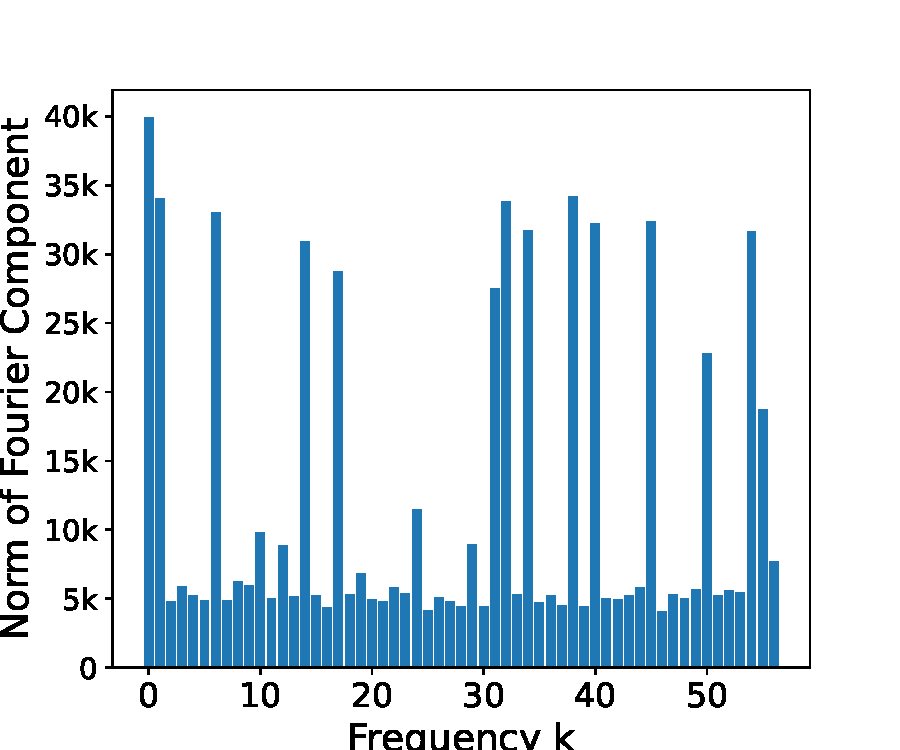
\includegraphics[width=0.4\textwidth]{grokking_iclr/figures/fourier_components.pdf}
            \end{center}
            \vspace{-10pt}
            \caption{Fourier components of the weights of the output layer of an MLP trained on addition mod 113. Grokking is induced with $\stablemax$ and without weight decay. \tolga{this figure is terribly cropped.}}
            \label{fig:fourier}
        \end{wrapfigure}
\end{comment}

 
Weight decay has been identified as potentially responsible for inducing the periodic structures in the weights studied in \cite{Nanda2023-hf}. In \cref{fig:fourier} we show that MLPs that grok without weight decay on modular addition show a similar sparsity in Fourier space as the one observed in \cite{Nanda2023-hf}. While these are very superficial results, they suggest that these structures can emerge without a weight decay--induced ``clean up'' phase as described in \cite{Nanda2023-hf}.

\section{Further Discussion on Conditions that Lead to Grokking}\label{app:further_discussion}
\subsection{L1 regularization and grokking}\label{app:l1_grokking}

%\paragraph{L1 regularization}
While it has been observed that L1 regularization can lead to grokking in some settings, \cite{Nanda2023-hf}
consistently found no grokking with L1 regularization and transformers and this setting has received substantially less attention than weight decay. 

We observe that \nlm scales the weights along their current direction. This means that larger weights are scaled more than small weights. However, while the sign of the gradient from L1 regularization depends on the sign of the weights, the magnitude of this gradient does not depend on the magnitude of the weights. This means that, particularly on deep networks or transformers with with large weights, L1 can sometimes be insufficient to prevent \nlm and the subsequent SC. 
%In Appendix \ref{app:l1_grokking} we show two examples, one where L1 regularization avoids SC and leads to grokking, and one where SC happens despite L1 regularization and grokking does not happen.

\subsection{Delaying generalization by scaling the weights} \label{app:scaling_weights}

\paragraph{Scaling the logits can delay generalization but not induce it} \cite{liu2023omnigrok}, \cite{Kumar2023-hz} and \cite{Lyu2023-ga} showed that an $\alpha$ parameter multiplying the logits can increase or reduce the delay in generalization. We highlight in \cref{fig:alpha_parameter} that this is true for cases where generalization happens even without changing the scale of the logits ($\alpha=1$). However, in most cases when using deeper networks or cross-entropy loss, models do not generalize by default without regularization and we are unable to induce grokking for any value of $\alpha$. 

We argue in \cref{sec:explain_existing_methods} that the observation in \cite{liu2023omnigrok}, \cite{Kumar2023-hz} and \cite{Lyu2023-ga} of grokking without regularization are due to the inductive bias of MSE loss which prevents NLM and leads to grokking in some settings for shallow networks.

\begin{figure}[t]
\centering
\begin{subfigure}{.33\textwidth}
  \centering
  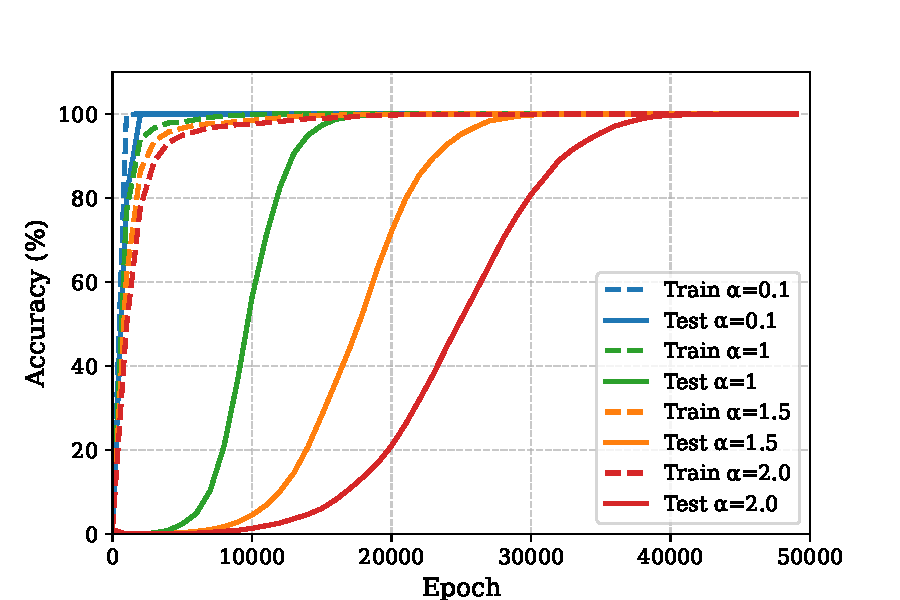
\includegraphics[width=\linewidth]{grokking_iclr_arxiv/figures/one_layer_MSE_alpha_sweep.pdf}
  \caption{MSE: 1 hidden layer}
\end{subfigure}%
\hfill
\begin{subfigure}{.33\textwidth}
  \centering
  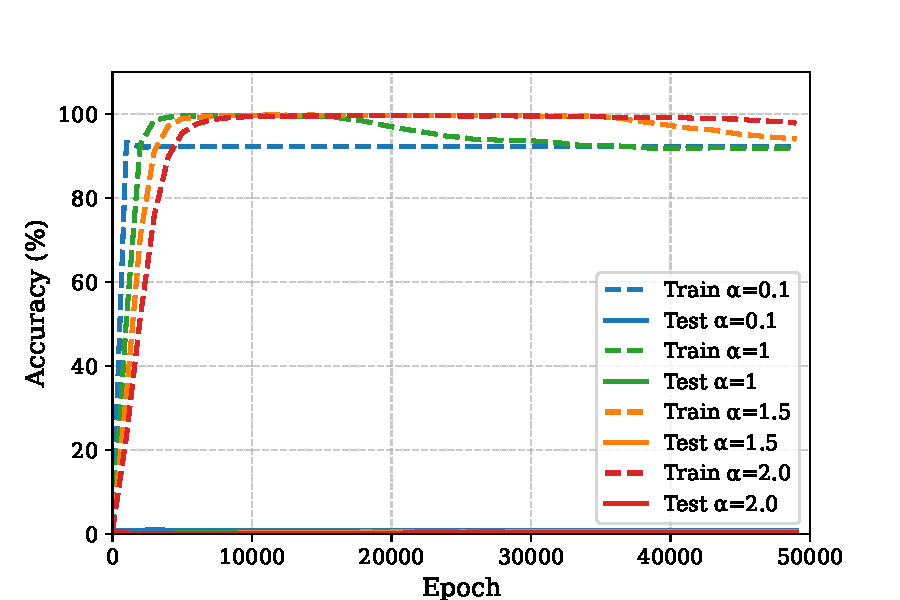
\includegraphics[width=\linewidth]{grokking_iclr_arxiv/figures/two_layer_MSE_alpha_sweep.pdf}
  \caption{MSE: 2 hidden layers}
\end{subfigure}%
\hfill
\begin{subfigure}{.33\textwidth}
  \centering
  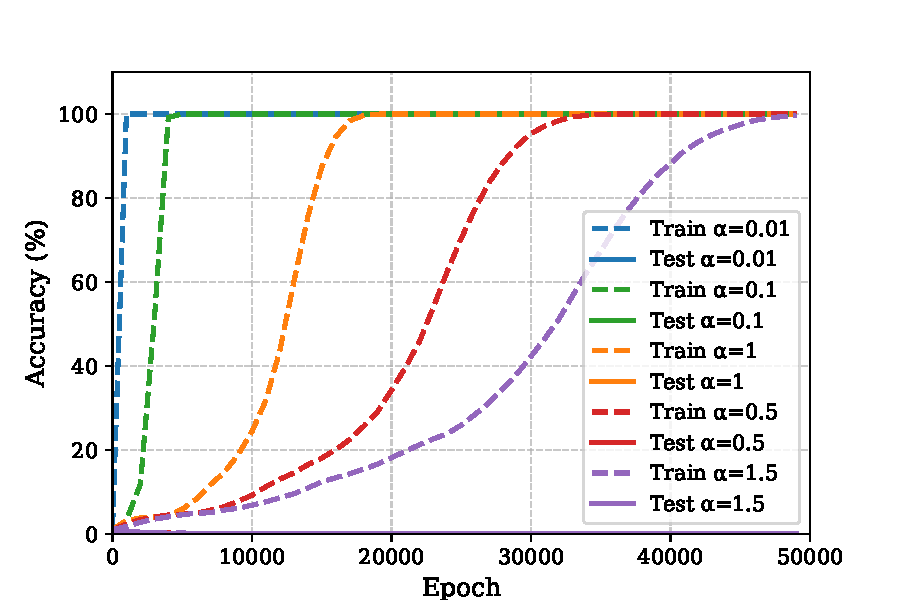
\includegraphics[width=\linewidth]{grokking_iclr_arxiv/figures/two_layer_cross_entropy_alpha_sweep.pdf}
  \caption{CE: 2 hidden layers}
\end{subfigure}
\caption{The $\alpha$ parameter controls generalization in settings where it happens by default. This is the case for shallow networks with MSE loss as shown in subplot (a). However, in deeper networks (b) or networks with CE loss and no regularization (c), $\alpha$ can control the time of over-fitting, but no value of $\alpha$ is enough to trigger grokking.}
\label{fig:alpha_parameter}
\end{figure}

\paragraph{Grokking on MNIST} We replicate the setting from \cite{liu2023grokking} of grokking on MNIST with cross-entropy loss and show that without weight decay, the scaling factor of the weights leads to significant FP errors, preventing grokking from happening until this is alleviated by weight decay. 

While SC explains why weight decay is needed to get the jump in performance observed in \cref{fig:mnist}. It could also explain why inducing grokking by scaling the weights is less effective when using SCE. While when using MSE loss, \cite{liu2023omnigrok} are able to induce full grokking from random level predictions to close to full training accuracy, the same does not seem to be possible when using SCE. In fact, we see in \cref{fig:mnist} that since the begining of training the rate of SC approaches 100\%. This could explain why the observations with cross-entropy loss are not the ones predicted by the lazy training theories outlined in \cite{Kumar2023-hz} which do not take limited floating point precision into account.

\begin{figure}[t]
    \vspace{-6mm}
    \centering
    \begin{subfigure}{.48\textwidth}
    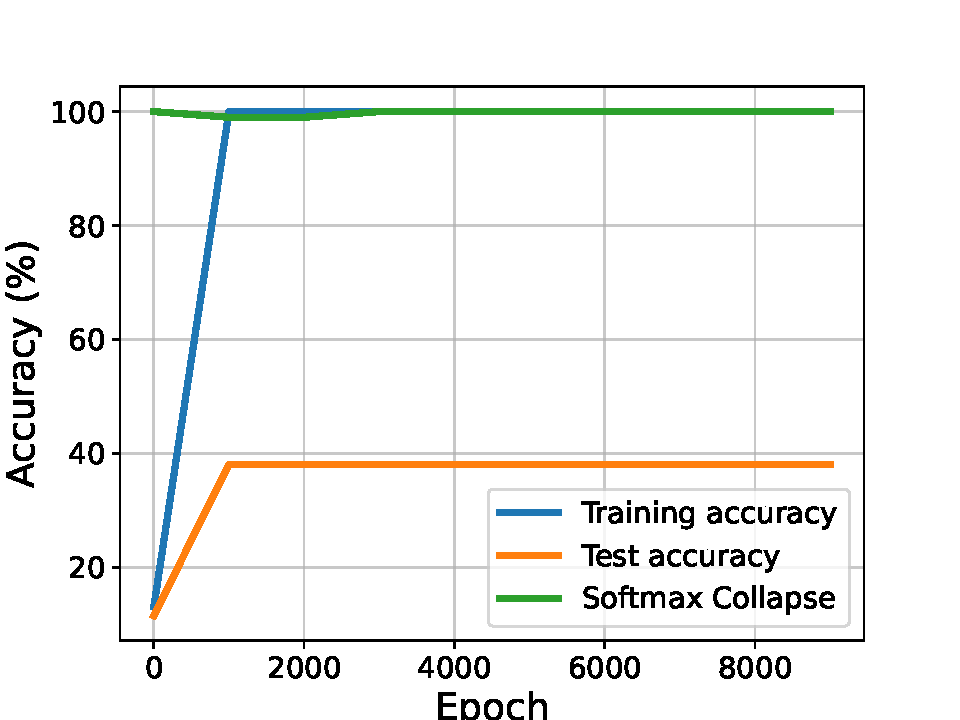
\includegraphics[width=\linewidth]{grokking_iclr_arxiv/figures/mnist_grokking.pdf}
        \caption{MLP without weight decay}
        \label{fig:mnist_witout_weight_decay}
    \end{subfigure}
    \begin{subfigure}{.48\textwidth}
    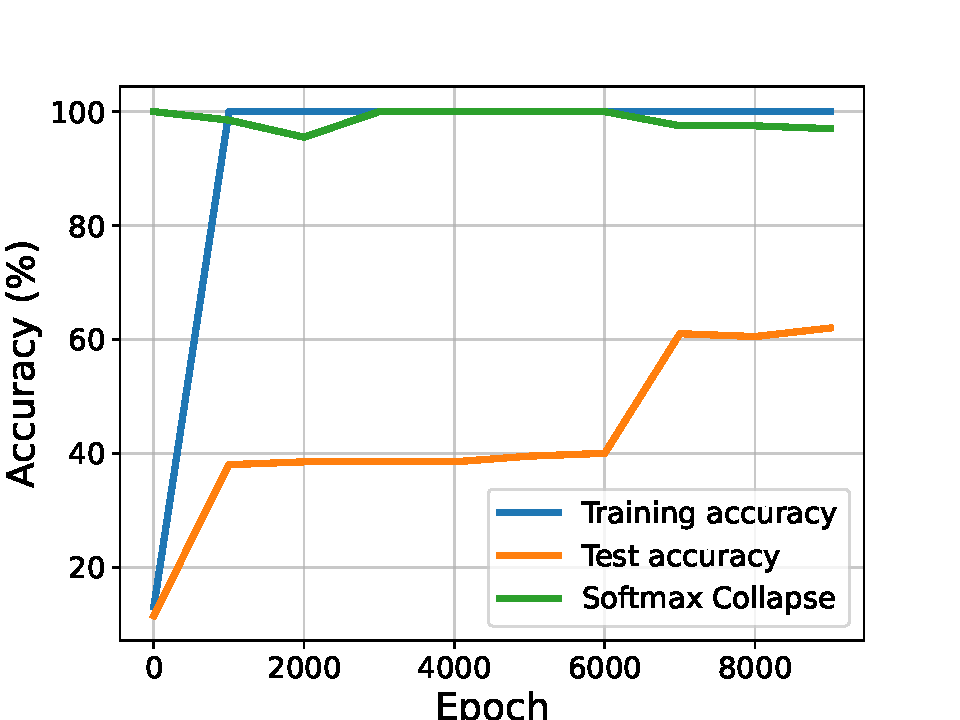
\includegraphics[width=\linewidth]{grokking_iclr_arxiv/figures/mnist_grokking_wd.pdf}
        \caption{MLP with weight decay.}
        \label{fig:mnist}
    \end{subfigure}
    \caption{Replicatting the grokking on MNIST for weight decay setting from \cite{liu2023grokking}. We find that MLPs with weights scaled up by 100 operate at the ``edge of numerical stability'' and in the absence of weight decay, SC eventually reaches 100\%, preventing any further generalization. When using weight decay, the weight norm is reduced, mittigating SC and eventually allowing for further generalization as the SC rate drops from 100\%.}

\end{figure}


\section{\ograd and Weight Decay}
In \cref{fig:wd_vs_ortho}, we provide a more in depth comparison of \ograd and weight decay. \cref{fig:wd_sweep} higlights that increasing the weight decay multiplier leads to a smaller delay in generalization, but only up to a point. In this concrete setting, a weight decay multiplier of 8, prevents the model from fully generalizing (\cref{fig:wd_sweep}). We then compare the best value of weight decay in this setting to \ograd, which does not require any hyper-parameter tuning. \cref{fig:vs_wd_seeds} shows that \ograd leads to faster grokking even when compared to a tuned value of weight decay. Note that the models with weight decay overfit immediately before grokking while \ograd reaches 100\% train and test accuracies almost at the same time.


\begin{figure}[t]
    \vspace{-5mm}
    \centering
    \begin{subfigure}{.48\textwidth}
    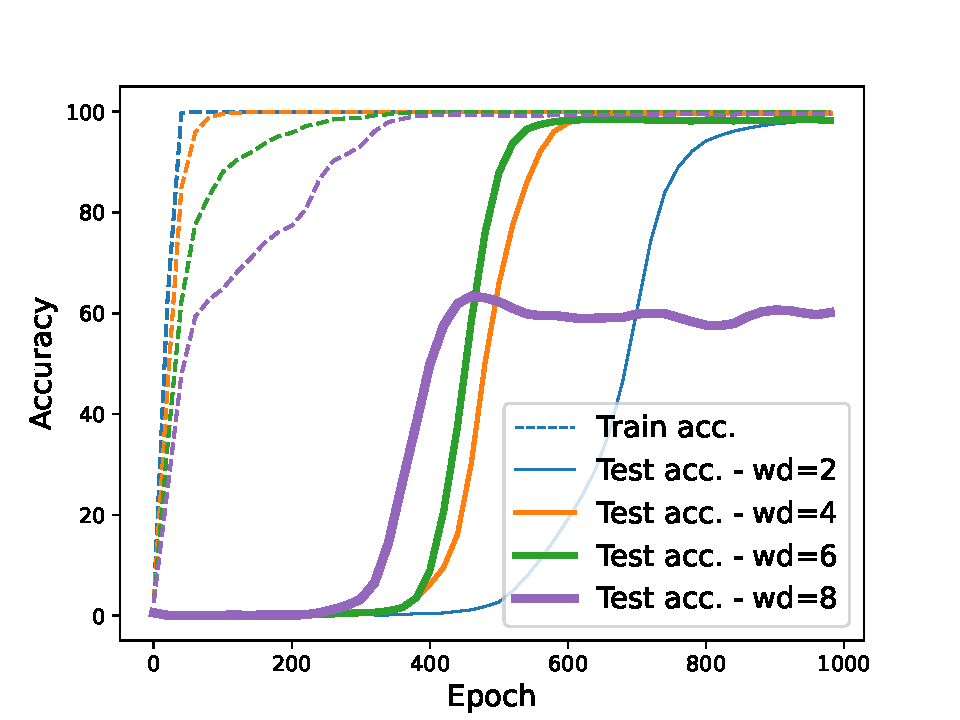
\includegraphics[width=\linewidth]{grokking_iclr_arxiv/figures/weight_decay_sweep.pdf}
        \caption{Sweep over values of weight decay}
        \label{fig:wd_sweep}
    \end{subfigure}
    \begin{subfigure}{.48\textwidth}
    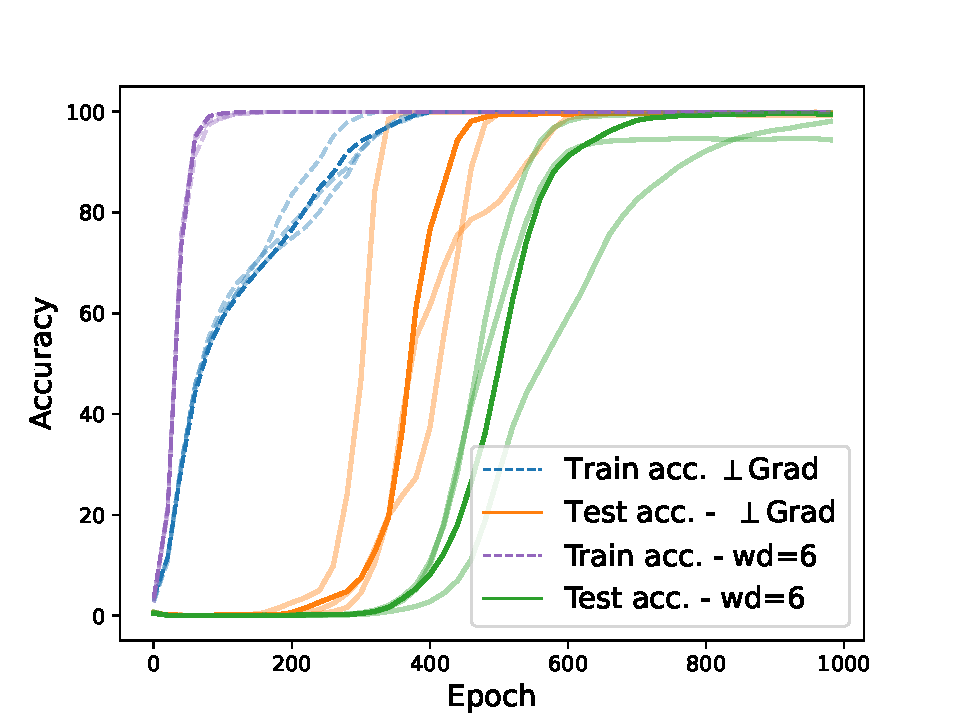
\includegraphics[width=\linewidth]{grokking_iclr_arxiv/figures/weight_decay_vs_orthograd_seeds.pdf}
        \caption{\ograd vs best performing wd model}
        \label{fig:vs_wd_seeds}
    \end{subfigure}
    \caption{Increasing weight decay (WD) for an MLP trained on modular addition with AdamW reduces the delay in generalization up to a point where WD prevents convergence \cref{fig:wd_sweep}. Without any tunable hyper-parameters and without WD, \ograd leads to grokking faster than the best model with WD \cref{fig:vs_wd_seeds}.}
    \label{fig:wd_vs_ortho}
\end{figure}

\section{Alternatives to $\stablemax$ in Preventing SC}
\begin{wrapfigure}[15]{R}{0.45\textwidth}
    \vspace{-7mm}
    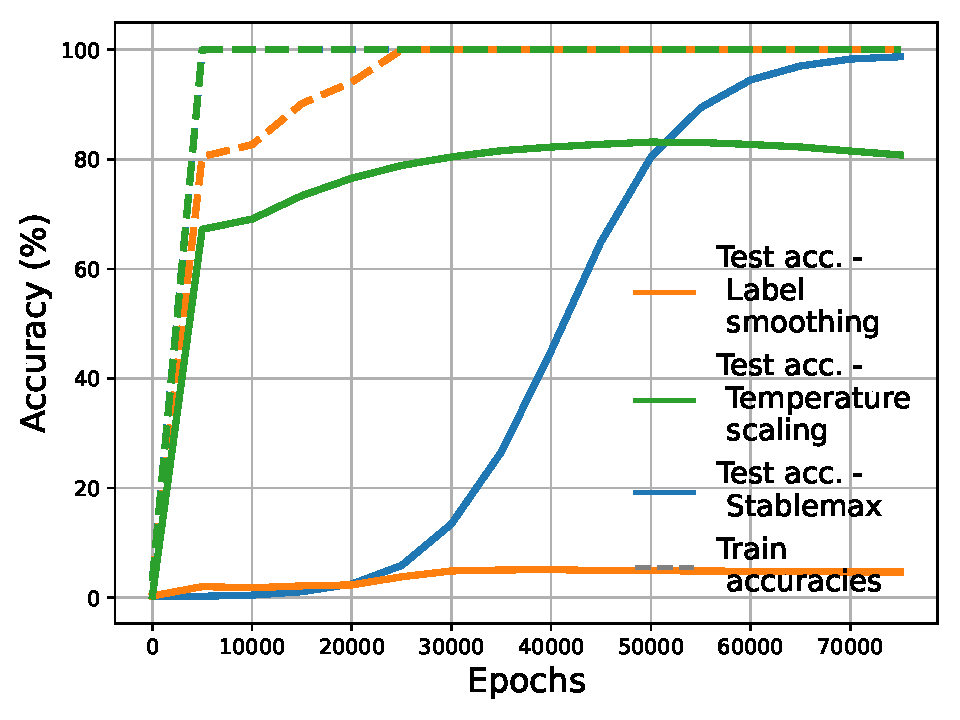
\includegraphics[width=\linewidth]{grokking_iclr_arxiv/figures/label_smoothing.pdf}
    \vspace{-8mm}
    \caption{$\stablemax$ prevents SC and leads to grokking while temperature scaling with $T=1e5$ only gradually delays SC, and label smoothing does prevent SC but at the cost of keeping the model from fully generalizing.}
    \label{fig:label_smoothing}
\end{wrapfigure}
While any intervention that prevents SC should lead to grokking or generalization, \cref{fig:label_smoothing} shows that scaling the temperature of the \softmax is not enough to prevent SC and label smoothing does prevent SC and lead to some generalization, but at the cost of introducing another inductive bias that prevents full generalization and leads to qualitatively different behavior. By comparison, the simple change introduced in Stablemax prevents SC and leads to grokking, serving as a validation for our hypothesis that gradient descent leads to grokking by default, unless this is stopped by SC.



\section{$\stablemax$ and \ograd \\ in Realistic Settings}
While Stablemax and \ograd are designed as interventions to show that preventing SC leads to grokking and preventing NLM leads to generalization (\cref{fig:teaser}), in this section we explore if these methods are applicable in more realistic settings like language modeling with GPT2-small or ResNets trained on image classification. We train GPT2-Small for 1 epoch on WikiText-103 using a batch size of 16, a block size of 512, a learning rate of $5e-4$ and a weight decay of 0.01 using AdamW. The architecture is the regular GPT2-Small architecture from \cite{radford2019language}, trained with a cosine schedule and 1000 steps of warmup.

For CIFAR10, CIFAR100 and Imagenet-1k \citep{ILSVRC15}, our baseline is a ResNet18 with SCE loss trained with SGD 0.9 momentum and $1e-4$ weight decay. We use standard data transformations such as random crop and random horizontal flip and a step learning rate scheduler every 30 epochs for a full training run of 100 epochs. With respect to this baseline we report results replacing the $\softmax$ with $\stablemax$ in the loss function, as well as replacing SGD with $\perp$SGD. Since test labels for Imagenet-1k are not publicly available, we use the validation set as a test set and tune hyper-parameters on a fraction of the training set.


\begin{figure}[t]
    \centering
    \begin{subfigure}{.32\textwidth}
    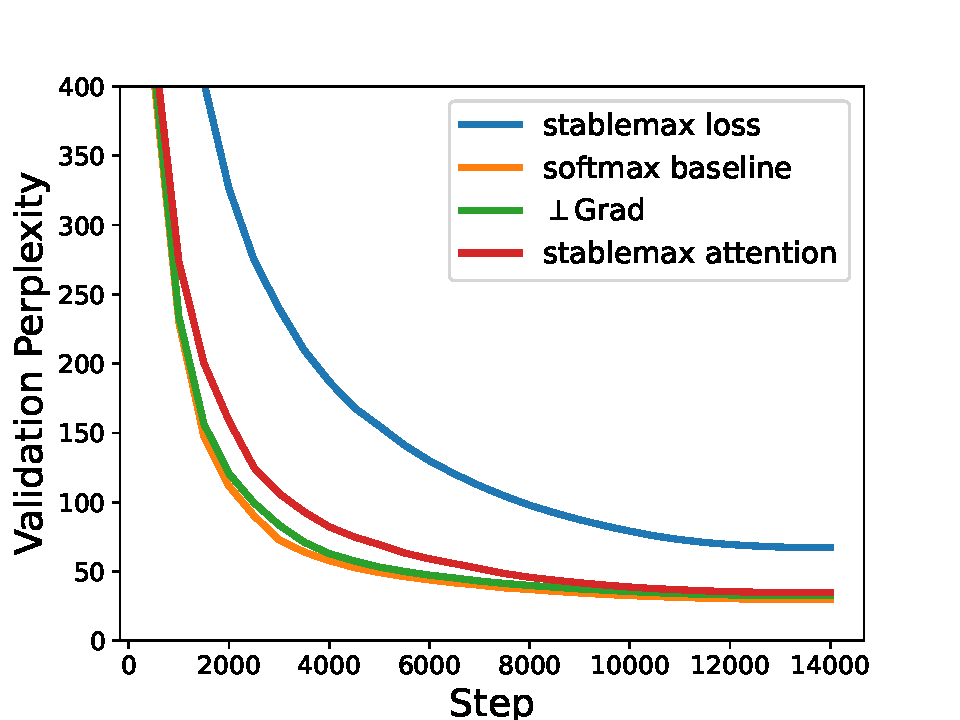
\includegraphics[width=\linewidth]{grokking_iclr_arxiv/figures/gpt2-small.pdf}
        \caption{GPT2-Small on WikiText2}
        \label{fig:gpt2_small}
    \end{subfigure}
    \hfill
    \begin{subfigure}{.32\textwidth}
    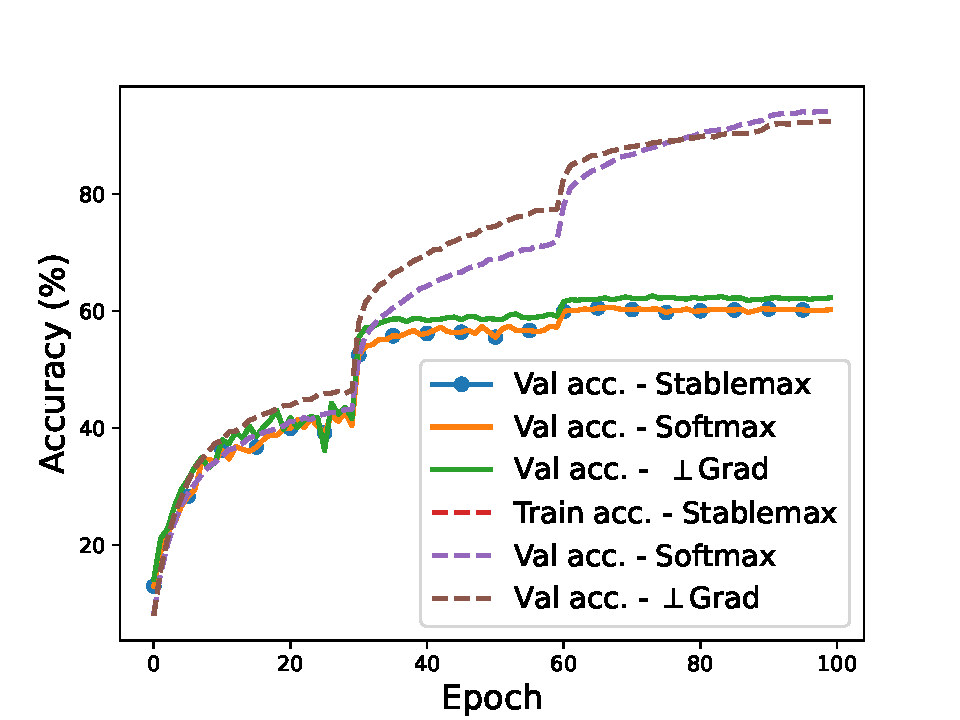
\includegraphics[width=\linewidth]{grokking_iclr_arxiv/figures/CIFAR100.pdf}
        \caption{ResNet18 on CIFAR100}
        \label{fig:cifar100_resnet18}
    \end{subfigure}
    \hfill
    \begin{subfigure}{.32\textwidth}
    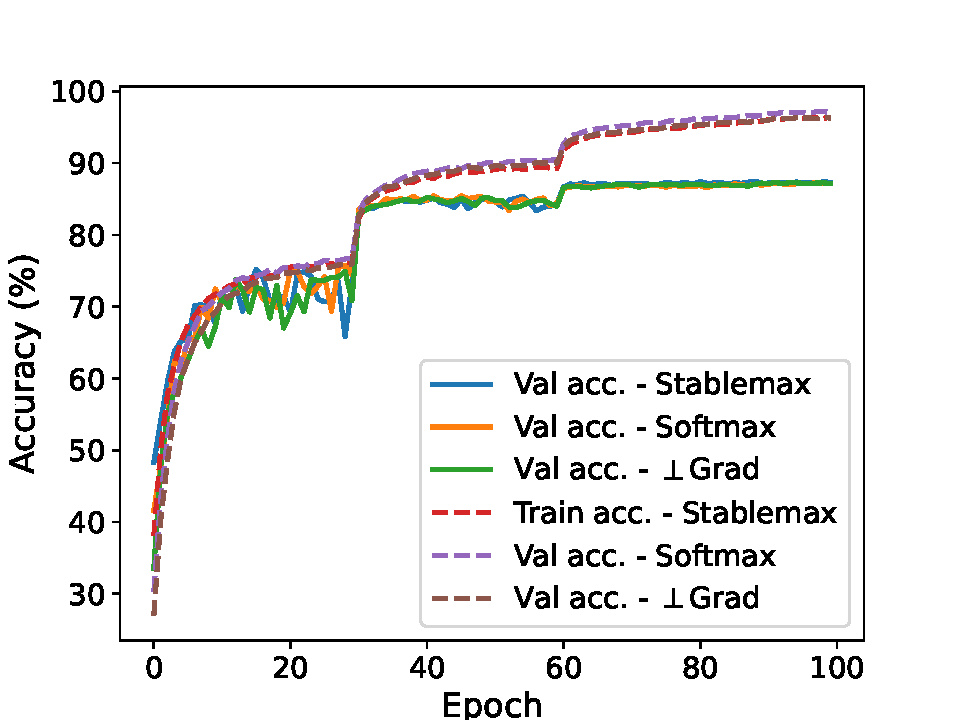
\includegraphics[width=\linewidth]{grokking_iclr_arxiv/figures/cifar10_resnet18.pdf}
        \caption{ResNet18 on CIFAR10}
        \label{fig:cifar10_resnet18}
    \end{subfigure}
    \caption{Comparing Stablemax and \ograd to AdamW with SCE on text data \cref{fig:gpt2_small} and image data \cref{fig:cifar10_resnet18}. For the GPT2-small results in \cref{fig:gpt2_small}, we also include the results of replacing the \softmax in the attention mechanism with $\stablemax$.}
\end{figure}

\begin{table}[h]
\centering
\begin{tabular}{@{}lcccc@{}}
\toprule
\textbf{Method}         & \textbf{CIFAR10} & \textbf{CIFAR100} & \textbf{ImageNet-1k} & \textbf{WikiText-103} (Top-5) \\ \midrule
Softmax CE              & $87.17\% \pm 0.2$ & $59.98\% \pm 0.4$  & $69.33\% \pm 0.04$              & $60.48\% \pm 0.04$                      \\
Stablemax CE            & $87.01\% \pm 0.2$ & $60.63\% \pm 0.4$  & $65.87\% \pm 0.22$             & $51.85\%  \pm 0.47$                  \\
\ograd                  & $87.22\% \pm 0.2$ & $62.69\% \pm 0.1$  & $68.95\% \pm 0.03$               & $59.64\%   \pm 0.04$                \\ 
\midrule
Stablemax Attention     & --                & --                 & --                   & $58.52\%   \pm 0.04$                   \\ \bottomrule
\end{tabular}
\label{tab:realistic_datasets}
\caption{For the methods introduced in this paper, we report accuracies with standard deviations across five seeds for the CIFAR datasets and three seeds for Imagenet-1k and WikiText-103. We report Top-5 accuracy in the case of WikiText-103.\vspace{-3mm}}
\end{table}


\section{SC and the Slingshot Effect}\label{app:slingshots}
\cite{slingshot-mechanism} observed that spikes in the training loss appear when training on grokking tasks with adaptive optimizers like Adam, and that these spikes can lead to generalization without weight decay. Although \cite{Nanda2023-hf} showed that slingshots are not necessary for grokking, it is still unclear what mechanism of adaptive gradient optimizers induces this behavior and why it leads to generalization. In light of the results in this paper, we believe that slingshots could lead to generalization because they prevent full SC. \cite{Nanda2023-hf} pointed out that something like SC could be responsible for these slingshots. One possible mechanism would be that zero gradients for some samples due to SC rapidly diminish the second-order moments leading to a large update or slingshot which moves the model away from full SC, although more research would be needed to properly show this.

While related to our work, slingshots are a different kind of instability which only appears with adaptive optimizers and can allow grokking. In contrast, we identify SC as a very specific issue in the \softmax that can affect any model trained with SCE, not only the ones trained with adaptive optimizers. Additionally SC prevents grokking whereas slingshots can lead to it. Wether and how slingshots are cause by SC remains an open research question, with some supporting evidence from \cite{Nanda2023-hf} which show that slingshots can disappear when using $float64$.

\section{Additional Details About Floating Points}
Beyond our main results, we found that in some cases, grokking could be stopped before SC due to the $\epsilon$ parameter in Adam being too large. While the $\epsilon$ term is designed to give numerical stability to the gradients, in settings with extremely low losses and gradients, the second order moments can be dominated by the $\epsilon$ term, putting an end to learning where it would have continued with a smaller $\epsilon$ value. This echoes the results in \cite{slingshot-mechanism} which shows that increasing $\epsilon$ halts slingshots and grokking, with \cite{Nanda2023-hf} also alluding to the $\epsilon$ parameter being important in some cases.  

Surprisingly, we also found that a simple re-implementation of $torch.nn.functional.log\_softmax$ that does not use the official CUDA kernels can lead the models to keep learning beyond the point where the loss is exactly 0 and some gradients should be 0 with appropriate calculation, outperforming the official implementation for grokking tasks. Learning eventually also stops in this setting and this seems more like a quirk of how gradients are calculated in PyTorch in the absence of an explicitly defined backward pass.




% \clearpage
% \citestyle{acmauthoryear}
% \bibliographystyle{ACM-Reference-Format}
% \bibliography{reference}
% \end{bibunit}
%%%%%% for TOG %%%%%% 

%%%%%% for arxiv %%%%%% 
%---------------------------------
\section{Introduction}
\label{sec:intro}
%---------------------------------


The popularity of powerful diffusion models has led to remarkable progress in the field of content generation. For instance, text-to-image (T2I) models are capable of generating diverse and vivid images from text prompts, encompassing various visual concepts. This great success can be attributed not only to the advancement of models but also to the availability of various image data over the Internet.
Constrastingly, text-to-video (T2V) models fall short of the data categories especially in styles, since existing videos predominantly feature photorealism. While these strategies, like initializing weights from well-trained T2I models or joint training with image and video datasets, can help mitigate this issue, the generated stylized videos generally suffer from degraded style fidelity. 
% Therefore, in addition to the classic problem of \textbf{style-content decoupling} in style transfer/preserving, stylized video generation also grapples with challenges including \textbf{a scarcity of stylized video data} and the \textbf{limited capabilities of T2V base models}.
Although significant success has been achieved in style transfer/preservation in T2I generation, the field of stylized video generation remains largely unexplored,
and effective solutions are yet to be discovered.
% As one of the pioneers, AnimateDiff~\cite{guo2023animatediff} can make impressive stylized videos by combining personalized T2I models~\cite{hu2022lora} (i.e. LoRA-tuned\cite{hu2022lora} or Dreambooth-tuned\cite{dreambooth} on Stable Diffusion\cite{ldm}) with pre-trained temporal blocks. However, each style requires additional finetuning on a small set of examples, which is inefficient and unable to support any style.

% \begin{figure}[!t]
%     \centering
%     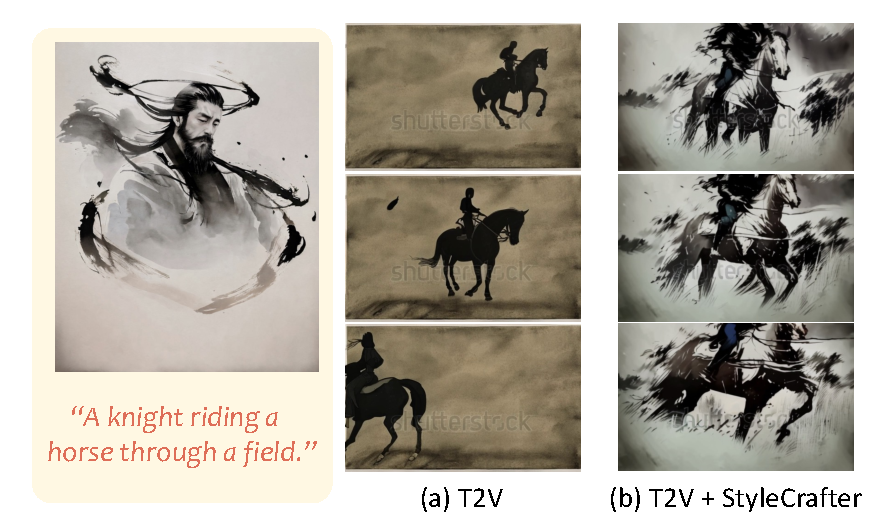
\includegraphics[width=\linewidth]{figures/motivation.pdf}\vspace{-0.5em}
%     \caption{Effect of adding style adapter to T2V models. (a) and (b) are results of Stable Diffusion~\cite{ldm} and VideoCrafter~\cite{chen2023videocrafter}. (c) is the result of VideoCrafter equipped with a style adapter. The content text prompt is "\textit{A knight riding a horse through the field}". For (a) and (b), the style prompt is generated from the style image using GPT4V~\cite{openai2023gpt4v}. \TODO{delete this figure}} 
%     \label{fig:motivation}\vspace{-0.5em}
% \end{figure}

In this paper, we propose StyleCrafter, a generic method that enhances pre-trained T2V models with a style control adapter, enabling text-to-video generation in any desired style by providing a reference image. 
% The advantages are twofold: (i) a style image offers stylistic feature guidance, complementing the stylization capabilities of T2V models in a zero-shot fashion; (ii) the reference image delivers a more accurate portrayal of the desired visual style compared to textual descriptions. 
Anyhow, it is non-trivial to achieve this goal. (i) as a classic problem of style transfer/preservation, the style control adapter requires to extract accurate style concepts from the reference image \textbf{in a content-style decoupled manner}. (ii) \textbf{the scarcity of open-source stylized videos} challenges the adaptation training of the T2V models.

Considering the scarcity of stylized videos, we propose to first train a style adapter to extract desired style concepts from images over image datasets, and then transfer the learned stylization ability to a T2V model with shared spatial weights through a tailor-made finetuning paradigm. The advantages are twofold: on the one hand, the adapter trained over stylized images can effectively extract the style concept from input images, eliminating the necessity for scarcely available stylized videos. On the other, a finetuning paradigm enables text-to-video models with better adaptation to the style concepts extracted from the previously trained style adapter, while avoiding degradation of temporal quality in video generation. 

To effectively capture the style features and promote content-style disentanglement, we adopt the widely used query transformer to extract style concepts from a single image. Particularly, we design a scale-adaptive fusion module to balance the influences of text-based content features and image-based style features, which helps generalization across various text and style combinations. During the training process, we employ carefully designed data augmentation strategies to enhance decoupled learning.

StyleCrafter efficiently generates high-quality stylized videos that align with the content of the texts and resemble the style of the reference images.
Comprehensive experiments are conducted to assess our proposed approach, demonstrating that it significantly outperforms existing competitors in both stylized image generation and stylized video generation. Furthermore, ablation studies offer a thorough analysis of the technical decisions made in developing the complete method, which provides valuable insights for the community.
Our contributions are summarized as follows:
\begin{itemize}
    \item We propose the concept of improving stylized generation for pre-trained T2V models by adding a style adapter.
    \item We explore an efficient network for stylized generation, which facilitates the content-style disentangled generation from text and image inputs. Our method attains notable advantages over existing baselines.
    \item We propose a training paradigm for generic T2V style adapter without requiring any stylized videos for supervision.
\end{itemize}
%---------------------------------
% \vspace{-0.5em}
\section{Related Works}
\label{sec:realtedworks}
%---------------------------------

\subsection{Text to Video Synthesis}
Text-to-video synthesis~(T2V) is a highly challenging task with significant application value, aiming to generate corresponding videos from text descriptions. Various approaches have been proposed, including autoregressive transformer~\cite{vaswani2017attention} models and diffusion models~\cite{DDPM, DDIM, nichol2021improved, song2020score}. 
% N{\"u}wa~\cite{wu2022nuwa} introduces a 3D transformer encoder-decoder framework to address various text-guided visual tasks including T2V generation.  Phenaki~\cite{villegas2022phenaki} presents a bidirectional masked transformer for compressing videos into discrete tokens, thereby enabling video generation. 
Video Diffusion Model~\cite{ho2022video} employs a space-time factorized U-Net to execute the diffusion process in pixel space. Imagen Video~\cite{ho2022imagen} proposes a cascade diffusion model and v-parameterization to enhance VDM. 
Another branch of techniques makes good use of pre-trained T2I models and further introduces some temporal blocks for video generation extension. CogVideo~\cite{hong2022cogvideo} builds upon CogView2~\cite{ding2022cogview2} and employs multi-frame-rate hierarchical training strategy to transition from T2I to T2V. Similarly,  Make-a-video~\cite{make-a-video}, MagicVideo~\cite{zhou2022magicvideo} and LVDM~\cite{he2022latent} inherit pretrained T2I diffusion models and extend them to T2V generation by incorporating temporal attention modules.
%Furthermore, some wrok have explored introducing additional control conditions in T2V diffusion models. Gen-1~\cite{esser2023structure} proposes a structure and content-guided VDM that utilizes frame-wise depth map to maintain structure. VideoComposer~\cite{wang2023videocomposer} focuses on video generation conditioned on multi-modal inputs, allowing textual, spatial, and temporal conditions.
%Follow Your Pose~\cite{ma2023follow} aims to generate pose-controllable character videos by employing a two-stage training process that exclusively utilizes image-pose and pose-free video. Nevertheless, example-based stylized video generation is seldom explored in the general video synthesis field.

\vspace{-0.7em}
\subsection{Stylized Image Generation}

Stylized image generation aims to create images that exhibit a specific style. Decoupling style and content is a classic challenge~\cite{tenenbaum2000separating}.
Early research primarily concentrated on image style transfer, a technique that involves the transfer of one image's style onto the content of another, requiring a source image to provide content. 
Traditional style transfer methods~\cite{hertzmann2001image,wang2004efficient, zhang2013style} employ low-level, hand-crafted features to align patches between content images and style images. Since Gatys et al.~\cite{gatys2016image} discovered that the feature maps in CNNs capture style patterns effectively, a number of studies~\cite{huang2017arbitrary, li2017universal, texler2020arbitrary, liu2021adaattn, an2021artflow, deng2022stytr2, zhang2022domain} have been denoted to utilize neural networks to achieve arbitrary style transfer. A common practice involves utilizing a pretrained VGG network~\cite{simonyan2014very} to extract style information or compute Gram matrix loss~\cite{gatys2016image} to enable self-supervised learning of visual styles.

As the field of generation models progressed, researchers began exploring stylized image generation for T2I models. Although T2I models can generate various artistic images from corresponding text prompts, words are often limited to accurately convey the stylistic elements in artistic works. Consequently, recent works have shifted towards example-guided artistic image generation. Several studies~\cite{dreambooth, shi2023instancebooth, customdiffusion, hu2022lora} developed various optimization techniques on a small collection of input images that share a common style concept. 
Inspired by Textural Inversion~(TI)~\cite{TI}, some methods~\cite{zhang2023inversion, ahn2023dreamstyler, sohn2023styledrop} propose to optimize a specific textual embedding to represent a certain style. Similarly to our work, IP-Adapter~\cite{ye2023ipadapter} trains an image adapter based on pretrained Stable Diffusion to adapt T2I models to image conditions. 
Although IP-Adapter can produce similar image variants, it fails to decouple style concepts from input images or generate images with other content through text conditions.


\vspace{-0.7em}
\subsection{Stylized Video Generation}
Building upon the foundation of stylized image generation, researchers have extended the concept to video style transfer and stylized video generation. Due to the scarcity of large-scale stylized video data, a common approach for video stylization involves applying image stylization techniques on a frame-by-frame basis. Before the advent of ML, researchers have explored methods for rendering specific artistic styles such as video watercolorization~\cite{bousseau2007video}. Early deep learning methods of video style transfer~\cite{ruder2016artistic,chen2017coherent,texler2020interactive,gao2020fast,jamrivska2019stylizing,deng2021arbitrary} apply style transfer in video sequences, generating stable stylized video sequences through the use of optical flow constraints. 
Additionally, Some video editing methods~\cite{wu2023tune,qi2023fatezero,khachatryan2023text2video,huang2023style,yang2023rerender,geyer2023tokenflow,yang2024fresco} based on pretrained T2I models also support text-guided video style transfer. Although these methods effectively improve temporal consistency, they often fail to handle frames with a large action span. Reliance on a source video also undermines flexibility. 
Similarly, certain image-to-video(I2V) methods~\cite{blattmann2023stable, xing2023dynamicrafter, xing2024tooncrafter} demonstrate capabilities in stylized video generation, particularly in the anime domain. However, I2V models still face challenges when tased with interpreting and animating highly artistic images, producing frames that veer towards realism, since real-world videos dominated its training data.

VideoComposer~\cite{wang2024videocomposer} focuses on controllable video generation, allowing multiple conditional input to govern the video generation, including structure, motion, style, etc. Although VideoComposer enables multiple controls including style, they fail to decouple style concepts, leading to limited visual quality and motion naturalness. AnimateDiff~\cite{guo2023animatediff} employs a T2I model as a base generator and adds a motion module to learn motion dynamics, which enables extending the success of personalized T2I models(e.g., LoRA~\cite{hu2022lora}, Dreambooth~\cite{dreambooth}) to video animation. However, the dependence on a personalized model restricts its ability to generate videos with arbitrary styles. Another associated research is Text2Cinemagraph~\cite{mahapatra2023text}, which utilizes pretrained text-to-image models to pioneer text-guided artistic cinemagraph creation. This approach surpasses some existing text-to-video models like VideoCrafter~\cite{chen2023videocrafter} in generating plausible motion in artistic scenes. Nevertheless, its main limitation lies in its confined applicability, primarily to landscapes, and its tendency to generate scanty motion patterns solely for fluid elements.

%---------------------------------
\vspace{-0.6em}
\section{Method}
\label{sec:method}
%---------------------------------

We propose a method to equip pre-trained Text-to-Video (T2V) models with a style adapter, allowing for the generation of stylized videos based on both a text prompt and a style reference image. The overview is illustrated in Figure~\ref{fig:overview}. In this framework, the textual description dictates the video content, while the style image governs the visual style, ensuring a disentangled control over the video generation process.
Given the limited availability of stylized videos, we employ a two-stage training strategy. Initially, we utilize an image dataset abundant in artistic styles to learn reference-based style modulation. Subsequently, adaptation finetuning on a mixed dataset of style images and realistic videos is conducted to improve the temporal quality of the generated videos.


%
\begin{figure}[t]
    \centering
    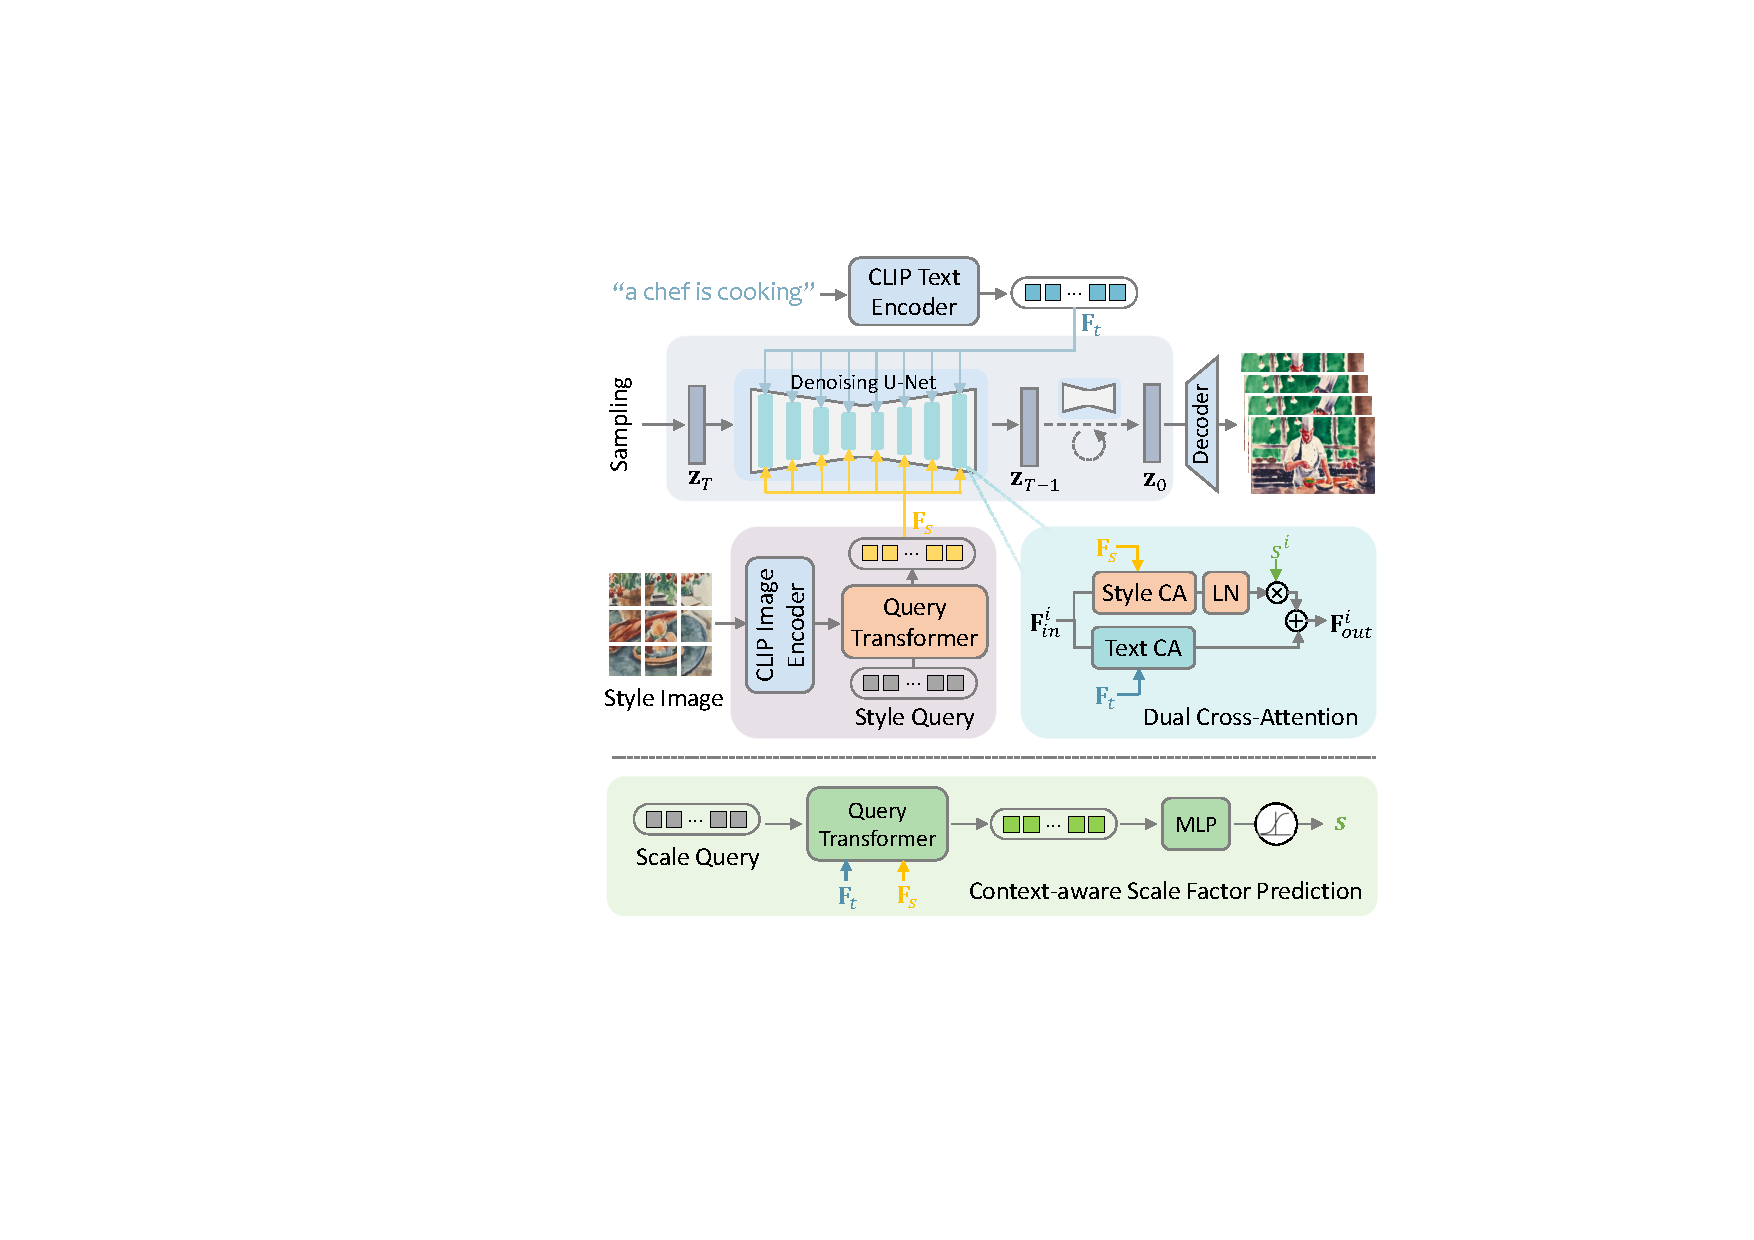
\includegraphics[width=0.95\linewidth]{figures/overview2.pdf}
    \vspace{-0.35cm}
    \caption{Overview of our proposed style adapter. It consists of three components, i.e. style feature extractor, dual cross-attention module, and context-aware scale factor predictor.}
    \label{fig:overview}
    \vspace{-1.4em}
\end{figure}


%---------------------------------
\vspace{-0.6em}
\subsection{Reference-Based Style Modulation}
\label{subsec:style_modulation}
%---------------------------------

Our style adapter serves to extract style features from the input reference image and infuse them into the backbone features of the denoising U-Net. As mainstream T2V models~\cite{chen2023videocrafter, chen2024videocrafter2, wang2023modelscope, wang2023lavie} are generally initialized from open-source T2I Models and trained with image and video datasets in a joint strategy, they support not only text-to-video generation but also retain the capacity for text-to-image generation. To overcome the scarcity of stylized videos, we propose to train the style adapter based on a pre-trained T2V model (i.e. VideoCrafter~\cite{chen2023videocrafter}) for stylized image generation under the supervision of stylistic images.

\vspace{-0.3em}
\paragraph{Content-Style Decoupled Data Augmentation.}
\label{sec:data_aug}
We use the stylistic images from two publicly available datasets, i.e. WikiArt~\cite{phillips2011wiki} and a subset of Laion-Aesthetics~\cite{schuhmann2022laion} (aesthetics score above 6.5). In the original image-caption pairs, we observe that the captions generally contain both content and style descriptions, and some of them do not match the image content well. To promote the content-style decoupling, we use BLIP\nobreakdash-2~\cite{li2023blip2} to regenerate captions for the images and remove certain forms of style description (e.g., \textit{a painting of}) with regular expressions.
In addition, as an image contains both style and content information, it is necessary to construct a decoupling supervision strategy to guarantee the extracted style feature free of content features. Although a stylistic image may contain different local style patterns~\cite{park2019arbitrary, huo2021manifold, chen2023tssat}, we regard that a large crop of an image(e.g. 50\% of the image) still preserves a similar style representation with the full image.
% We regard that every local regions of a stylistic image share the same style representation, which not only reflects on texture and color theme but also on the structure and perceptual semantics. 
Based on this insight, we process each stylistic image to obtain the target image and style image through different strategies: for target image, we scale the shorter side of the image to 512 and then crop the target content from the central area; for style image, we scale the shorter side of the image to 800 and randomly crop a local patch with $512 \times 512$. This approach reduces the overlap between the style reference and generation target, while still preserving the global style semantics complete and consistent.

\vspace{-0.3em}
\paragraph{Style Embedding Extraction.}
CLIP~\cite{radford2021learning} has demonstrated remarkable capability in extracting visual features from open-domain images. To capitalize on this advantage, we employ a pre-trained CLIP image encoder as a feature extractor. Specifically, we utilize both the global semantic token and the full $256$ local tokens (i.e., from the final layer of the Transformer) since our desired style embedding should not only serve as an accurate style trigger for the T2V model, but also provide auxiliary feature references.
As image tokens encompass both style and content information, we further employ a trainable Query Transformer (Q-Former)~\cite{li2023blip2} to extract style embedding $\mathbf{F}_s$. We create $N$ learnable style query embeddings as input for the Q-Former, which interact with image features through self-attention layers.
%We define style as the synthesized information present in an image that characterizes its overall aesthetic, independent of content. It encompasses both high-level aesthetic semantic information, such as composition, artistic conception, and color scheme, as well as low-level texture information, including specific brush stokes, lines, and surface details.
Note that this is a commonly adopted architecture for visual condition extraction~\cite{li2023blip2, shi2023instancebooth,ye2023ipadapter, xing2023dynamicrafter}. But it is the style-content fusion mechanism that makes our proposed design novel and insightful for style modulation, as detailed below.

\begin{figure}[t]
    \centering
    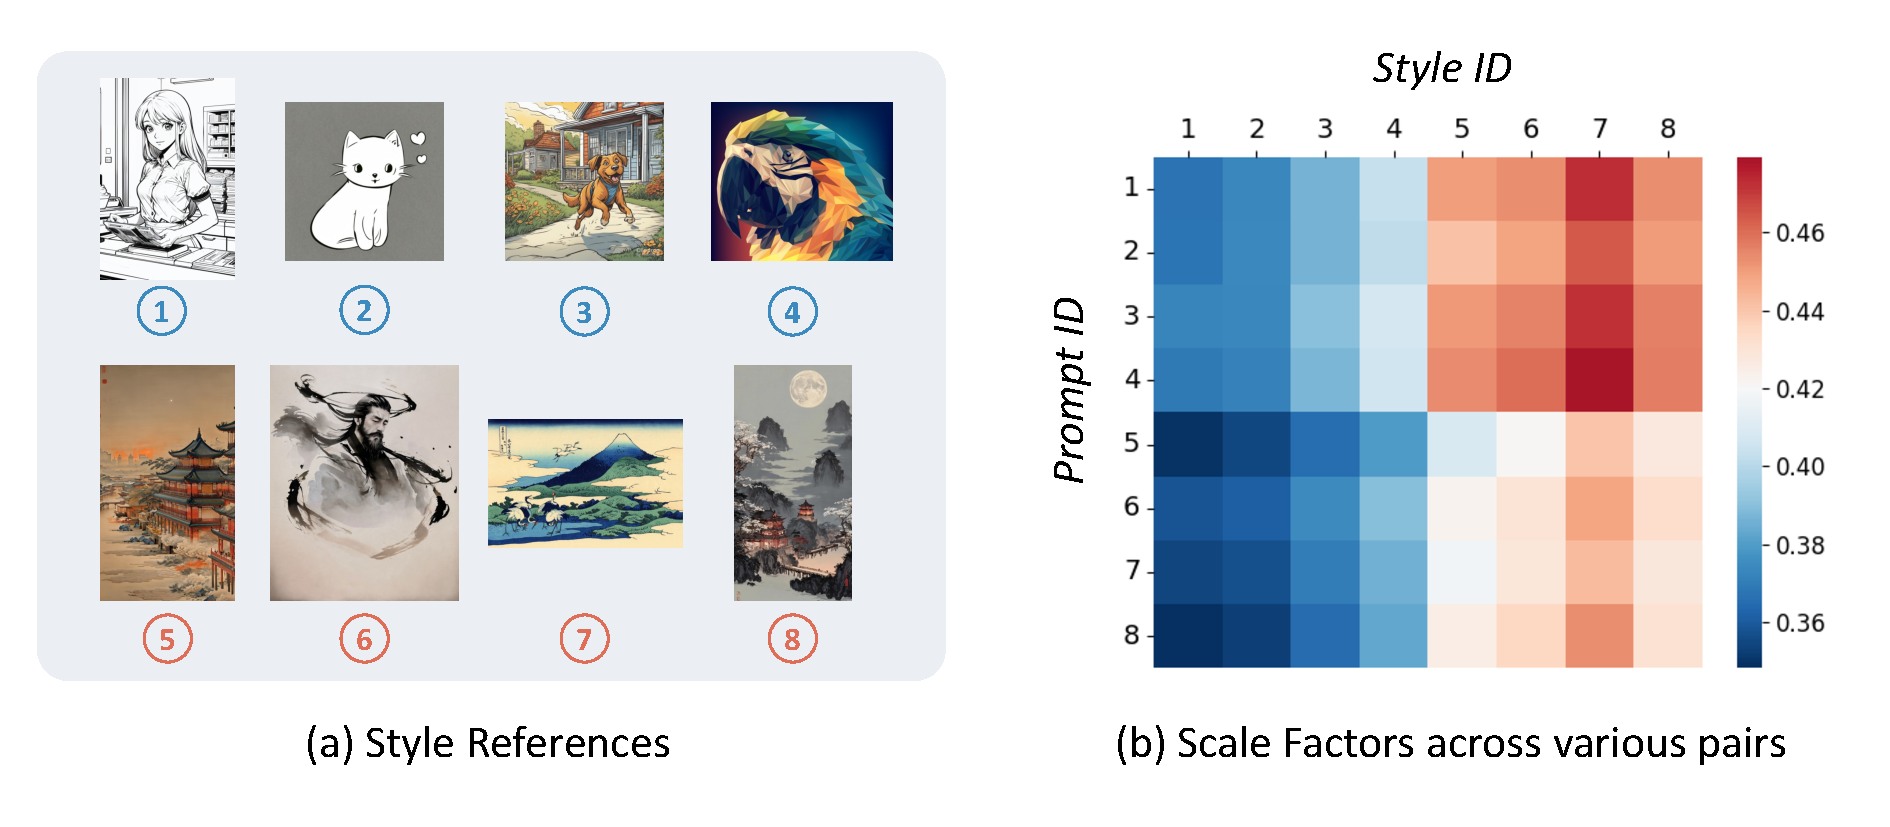
\includegraphics[width=\linewidth]{figures/scale_factor_viz.pdf}
    \vspace{-1.0cm}
    \caption{Illustration of content-style fusion scale factors across multiple input pairs. Four short prompts(less than 5 words) with prompt id $\in [1, 4]$ and four long prompts(more than 8 words) with prompt id $\in [5, 8]$ are randomly selected. Results indicate that shorter prompts and images with richer style-semantics tend to have relatively higher scale factors.} 
    \label{fig:scale_factor_viz}
    \vspace{-0.35cm}
\end{figure}

\paragraph{Adaptive Style-Content Fusion.}
\label{sec:fusion}
With the extracted style embedding, there are two ways to combine the style and text conditions, including (i) \textit{attach-to-text}~\cite{composer,gligen,ramesh2022hierarchical}: attach the style embedding to the text embedding and then interact with the backbone feature via the originally text-based cross-attention as a whole; (ii) \textit{dual cross-attention}~\cite{wei2023elite,ye2023ipadapter}: adding a new cross-attention module for the style embedding and then fuse the text-conditioned feature and style-conditioned feature.
According to our experiment (see Sec.~\ref{subsec:ablation}), solution (ii) surpasses solution (i) in disentangling the roles of text and style conditions, therefore we have adopted it as our final solution. The formula can be written as:
\vspace{-0.3em}
\begin{equation}
    \mathbf{F}_{out}^{i} = \text{TCA}(\mathbf{F}_{in}^i, \mathbf{F}_t) + s^i * \text{LN}(\text{SCA}(\mathbf{F}_{in}^i, \mathbf{F}_s)),
\end{equation}
where $\mathbf{F}_{in}^i$ denotes the backbone feature of layer $i$, LN denotes layer normalization, and TCA and SCA denote text-based cross attention and style-based cross attention respectively. $s^i$ is a scale factor learned by a context-aware scale factor prediction network, to balance the magnitudes of text-based feature and style-based feature.
The motivation is that different stylistic genres may have different emphasis on content expression. For example, the abstract styles tend to diminish the concreteness of the content, while realism styles tend to highlight the accuracy and specificity of the content. So, we propose a context-aware scale factor prediction network to predict fusion scale factors according to the input contexts.
Specifically, we create a learnable factor query, it interacts with textual features $\mathbf{F}_t$ and style features $\mathbf{F}_s$ to generate scale features via a Q-Former and then project it into layer-wise scale factors $\mathbf{s} \in \mathbb{R}^{16}$.
Figure~\ref{fig:scale_factor_viz} illustrates the learned scale factors across multiple contexts. It shows that the adaptive scale factors have a strong correlation with style genres while also depending on the text prompts. Style references with rich style-semantics(i.e., ukiyo-e style) typically yield higher scale factors to emphasize style; while complex prompts tend to produce lower scale factors to enhance content control.  This is consistent with our hypothesis to motivate our design.


%---------------------------------
\vspace{-0.5em}
\subsection{Temporal Adaptation to Stylized Features}
\label{subsec:temp_adaptation}
%---------------------------------

Given a pre-trained T2V model, the style adapter trained on image dataset works well for stylized image generation. However, it still struggles to generate satisfactory stylized videos, which is vulnerable to temporal jittering and visual artifacts.
The possible causes are that the cross-frame operations, i.e. temporal self-attention, do not involve in the process of stylized image generation, and thus induce incompatible issues. So, it is necessary to finetune the temporal self-attention with the style adapter incorporated.
Following the practice of T2V image and video joint training, the finetuning is performed on the mixed datasets of stylistic images and photorealistic videos. This is an adaptation training of temporal blocks while the other modules remain frozen, and the model converges efficiently.

\vspace{-0.5em}
\paragraph{Classifier-Free Guidance for Multiple Conditions.}
Unlike T2I models, video models exhibit a higher sensitivity to style guidance due to their limited stylized generation capabilities. Using a unified $\lambda$ for both style and context guidance may lead to undesirable generation results. Regarding this, we adopt a more flexible mechanism for multiple conditions classifier-free guidance. Building upon the vanilla text-guided classifier-free guidance, which controls context alignment by contrasting textual-conditioned distribution $\epsilon(z_t, c_t)$ with unconditional distribution $\epsilon(z_t, \varnothing)$, we introduce the style guidance with $\lambda_s$ by emphasizing the difference between the text-style-guided distribution $\epsilon(z_t, c_t, c_s)$ and the text-guided distribution $\epsilon(z_t, c_t)$. The complete formulation is as below:
\begin{equation}
    \begin{aligned}
        \hat{\epsilon}(z_t, c_t, c_s) = \epsilon(z_t, \varnothing) &+ \lambda_s(\epsilon(z_t, c_t, c_s) - \epsilon(z_t, c_t)) \\
        &+ \lambda_t(\epsilon(z_t, c_t) - \epsilon(z_t, \varnothing)),
    \end{aligned}
\end{equation}
where $c_t$ and $c_s$ denote textual and style condition respectively. $\varnothing$ denotes using no text or style conditions.
In our experiment, we follow the recommended configuration of text guidance in VideoCrafter~\cite{chen2023videocrafter}, setting $\lambda_t = 15.0$, while the style guidance is configured with $\lambda_s = 7.5$ empirically. Similarly, we set $\lambda_t = 7.5$ and $\lambda_s = 5.0$ for style-guided image generation.






%---------------------------------
\vspace{-0.3em}
\section{Experimental Results}
\label{sec:result}
%---------------------------------

%---------------------------------
\subsection{Experimental settings}
\label{subsec:experiment_setting}
%---------------------------------

\paragraph{Implementation Details.} 
We adopt the VideoCrafter~\cite{chen2023videocrafter} as our base T2V model, which shares the same spatial weights with Stable Diffusion 2.1. We first train the style modulation on image dataset, i.e. WikiArt~\cite{phillips2011wiki} and Laion-Aesthetics-6.5+~\cite{schuhmann2022laion} for 40k steps with a batch size of 32 per GPU.  In the second stage, we froze the style modulation part and only train temporal blocks of VideoCrafter, we jointly train image datasets and video datasets(subset of WebVid-10M~\cite{bain2021frozen}) for 20k steps with a batch size of 1 on video data and 16 on image data, sampling image batches with a ratio of 20\%. The training process is performed on 8 A100 GPUs and can be completed within 3 days. Furthermore, to ensure a fair comparison with some SDXL-based models~\cite{ye2023ipadapter, hertz2023style} on stylized image generation, we also trained the first stage of StyleCrafter on SDXL~\cite{podell2023sdxl}. 
%The overall training process takes about 5 days on 8$\times$V100.

% We train the style adapter on xx for xx epoches, with xx frozen and only train xxxx. In the second stage, xxx. We use xx optimizer and learning rate of xxxx. Also, training dataset.  \TODO{complete this part}

\paragraph{Testing Datasets.}
\label{sec:test_dataset}
To evaluate the effectiveness and generalizability of our method, we construct testsets comprising content prompts and style references. For content prompts, we use GPT-4~\cite{openai2023gpt4v} to generate recognizable textual descriptions from four meta-categories~(human, animal, object, and landscape). We manually filter out low-quality prompts, retaining 20 image prompts and 12 video prompts. For style references, we collect 20 stylized images and 8 sets of style images with multi-reference~(each contains 5 to 7 images in similar styles) from the Internet. In total, the test set contains 400 pairs for stylized image generation, and 300 pairs for stylized video generation (240 single-reference pairs and 60 multi-reference pairs). Details are available in the supplementary materials.

% 1. Content Prompt(generated from GPT4)
% 2. Style Image(selected from internet)
% 3. Content Image(generated from SD, for some style transfer method)
% 4. Style Prompt(generated from GPT4-v, for sd and video-crafter)

\paragraph{Evaluation Metrics.}
\label{sec:eval_metrics}
Following previous practice~\cite{zhang2023inversion, sohn2023styledrop, wang2023styleadapter}, we employ CLIP-based~\cite{radford2021learning} scores and DINO-based~\cite{caron2021emerging} scores to measure the text alignment and style conformity. Following EvalCrafter~\cite{liu2023evalcrafter}, we measure the temporal consistency of video generation by (i) calculating clip scores between contiguous frames and (ii) calculating the warping error on every two frames with estimated optical flow. 
Note that these metrics are not perfect. For example, one can easily achieve a close-to-1 style score by entirely replicating the style reference. Similarly, stylized results may yield inferior text scores compared to realistic results, even though both accurately represent the content descriptions. We recommend a comprehensive consideration of both CLIP-based text scores and style scores, rather than relying solely on a single metric.

\paragraph{User Preference Study.}
In addition to quantitative analysis, we conducted a user study to make comparisons among our method, VideoCrafter, Gen-2, and AnimateDiff in the context of single-reference and multi-reference stylized video generation. Users are instructed to select their preferred option based on style conformity, temporal quality, and all options fulfill text alignment for each comparison pair. We randomly chose 15 single-reference pairs and 10 multi-reference pairs, collecting 1125 votes from 15 users. 
Further details can be found in the supplementary materials.

%
\begin{table*}[!t]
\centering
%\setlength{\tabcolsep}{3.0pt}
% \renewcommand\arraystretch{1.5}
\caption{Quantitative comparison on single-reference style-guided T2I generation. We conduct evaluation on a test set of 400 pairs. \textbf{Bold}: Best. }
\label{tab:img_quan_clip}
\vspace{-1em}
\resizebox{0.93\linewidth}{!}{
  \begin{tabular}{ccccccccc} % {@{}lc@{}}
    \toprule
     \multirow{2}{*}{Method} & \multicolumn{4}{c}{\textbf{Stable Diffusion 2.1 based}} & \multicolumn{4}{c}{\textbf{SDXL based}} \\
    \cmidrule(lr){2-5}\cmidrule(lr){6-9}
     & Dreambooth & InST & SD* & Ours & IP-Adapter-Plus & Style-Aligned & SDXL* & Ours(SDXL)  \\
    \midrule
    \texttt{CLIP-Text} $\uparrow$ & \textbf{0.3047}  & 0.3004 & 0.2766 & 0.3028 & 0.2768 & 0.2254 & 0.2835 & \textbf{0.2918} \\
    \texttt{CLIP-Style} $\uparrow$ & 0.3459 & 0.3708 & 0.4183 & \textbf{0.4836} & 0.5182 & 0.5515 & 0.4348 & \textbf{0.5615} \\
    \texttt{DINO-Style} $\uparrow$ & 0.2278 & 0.2587 & 0.2890 & \textbf{0.3652} & 0.4367 & 0.4395 & 0.2912 & \textbf{0.4514} \\
    \bottomrule
  \end{tabular}
}
\end{table*}



%---------------------------------
\subsection{Style-Guided Text-to-Image Generation}
\label{subsec:image_eval}
%---------------------------------

As mentioned in Sec.~\ref{subsec:style_modulation} and Sec.~\ref{subsec:experiment_setting}, our proposed method also supports to generate stylized images~(using model before temporal finetuning). We are interested to evaluate our method against state-of-the-art style-guided T2I synthesis methods, which are better-established than video counterparts. The competitors include optimization-based methods like DreamBooth~\cite{dreambooth}, inversion-based methods such as InST~\cite{zhang2023inversion} and Style-Aligned~\cite{hertz2023style}, and adapter-based methods like IP-Adapter-Plus~\cite{ye2023ipadapter}. Besides, we consider two unique competitors: SD*~\cite{ldm} and SDXL*~\cite{sdxl}~(text-to-image models equipped with GPT-4V~\cite{openai2023gpt4v}, where GPT-4V generates textual descriptions about the reference's style and merges them with content prompts as input for models). This comparison aims to validate the advantages of employing image conditions to enhance stylized generation instead of relying solely on text conditions.
Implementation details of competitors are available in supplementary materials.
% For each style, DreamBooth and CustomDiffusion are optimized with the provided single reference image to learn the customized concept of style.
%This setting may degrade their performance (because they usually requires 5~20 images to learn a concept) but it is fair comparison since all the methods are only provided with a single style image.

The quantitative comparison is tabulated in Table~\ref{tab:img_quan_clip}. 
% Although our method achieved the best performance on both metrics, we would like to emphasise that clip-based metrics are imperfect.As discussed in Sec.~\ref{sec:eval_metrics}, the CLIP-Text is measured by the similarity between content text embedding and stylized image embedding, the stylistic appearance actually hinders the metric in some extent, which makes those methods with weak stylistic effects (i.e. close to photorealism) achieve superior scores. 
Results reveal that Dreambooth~\cite{dreambooth} and InST~\cite{zhang2023inversion} struggle to accurately capture the style from various style references and exhibit low style conformity. SD*~\cite{ldm} and SDXL~\cite{sdxl} demonstrate good stylistic ability but still fail to reproduce the style of the reference image, possibly because of the text’s inherent clumsiness in expressing specific styles despite utilizing the powerful GPT4V for visual style understanding. IP-Adapter~\cite{ye2023ipadapter} and style-aligned~\cite{hertz2023style} generate aesthetically pleasing images, while their style-content decoupled learning is not perfect and exhibits limited control over content.
In contrast, our method efficiently generates high-quality stylized images that align with the content of the texts and resemble the style of the reference image. Our method demonstrates stable stylized generation capabilities when dealing with various types of prompts.


%---------------------------------
\subsection{Style-Guided Text-to-Video Generation}
\label{subsec:video_eval}
%---------------------------------

\begin{figure*}[t!]
    \centering
    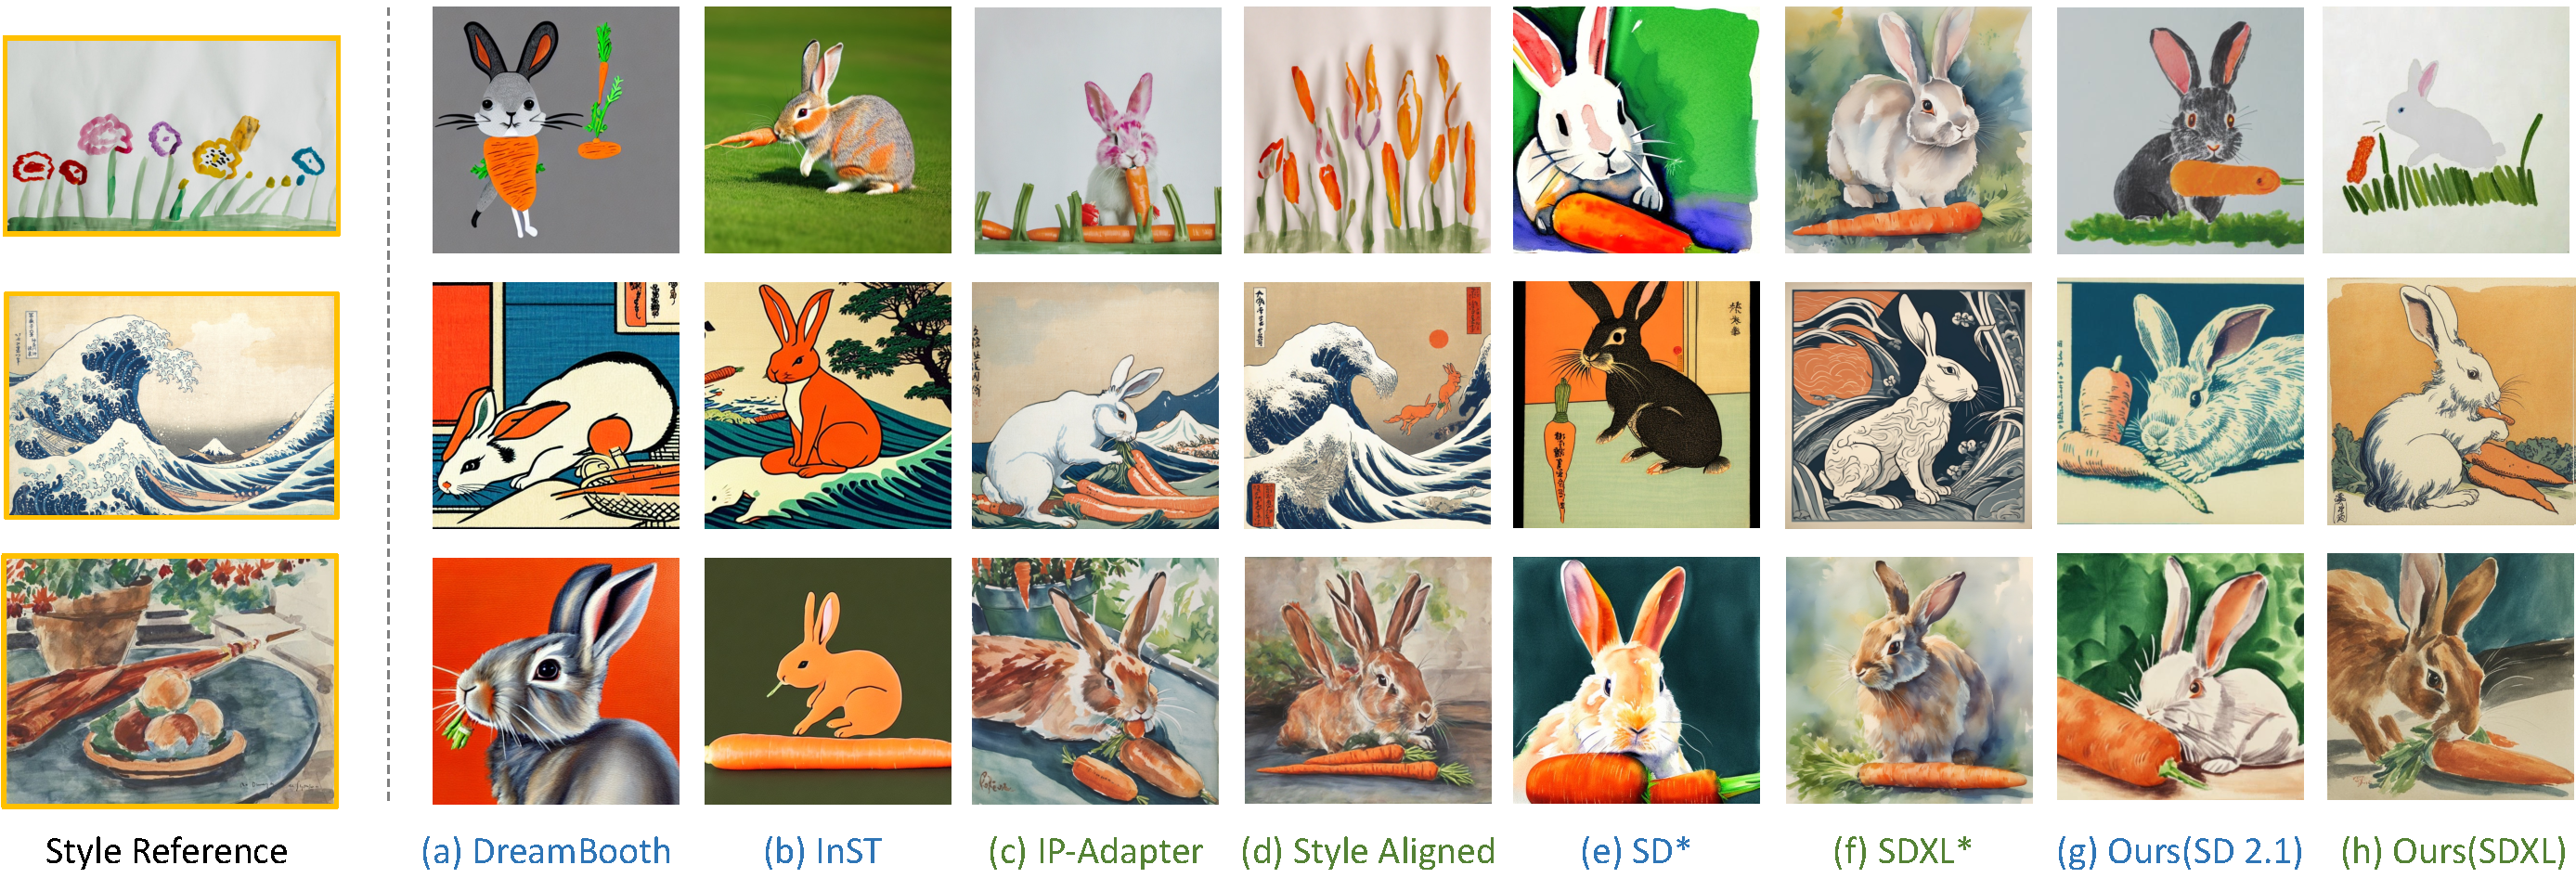
\includegraphics[width=0.87\linewidth]{figures/comp_image.pdf}
    \vspace{-1em}
    % \vspace{-2em}
    \caption{Visual comparison on style-guided T2I generation. \textcolor[RGB]{46, 117, 182}{Blue}: methods based on SD 2.1. \textcolor[RGB]{84, 130, 53}{Green}: based on SDXL. Prompt: A rabbit nibbling on a carrot.} 
    \label{fig:result_img}
    \vspace{-1em}
\end{figure*}
%
\begin{figure*}[!h]
    \centering
    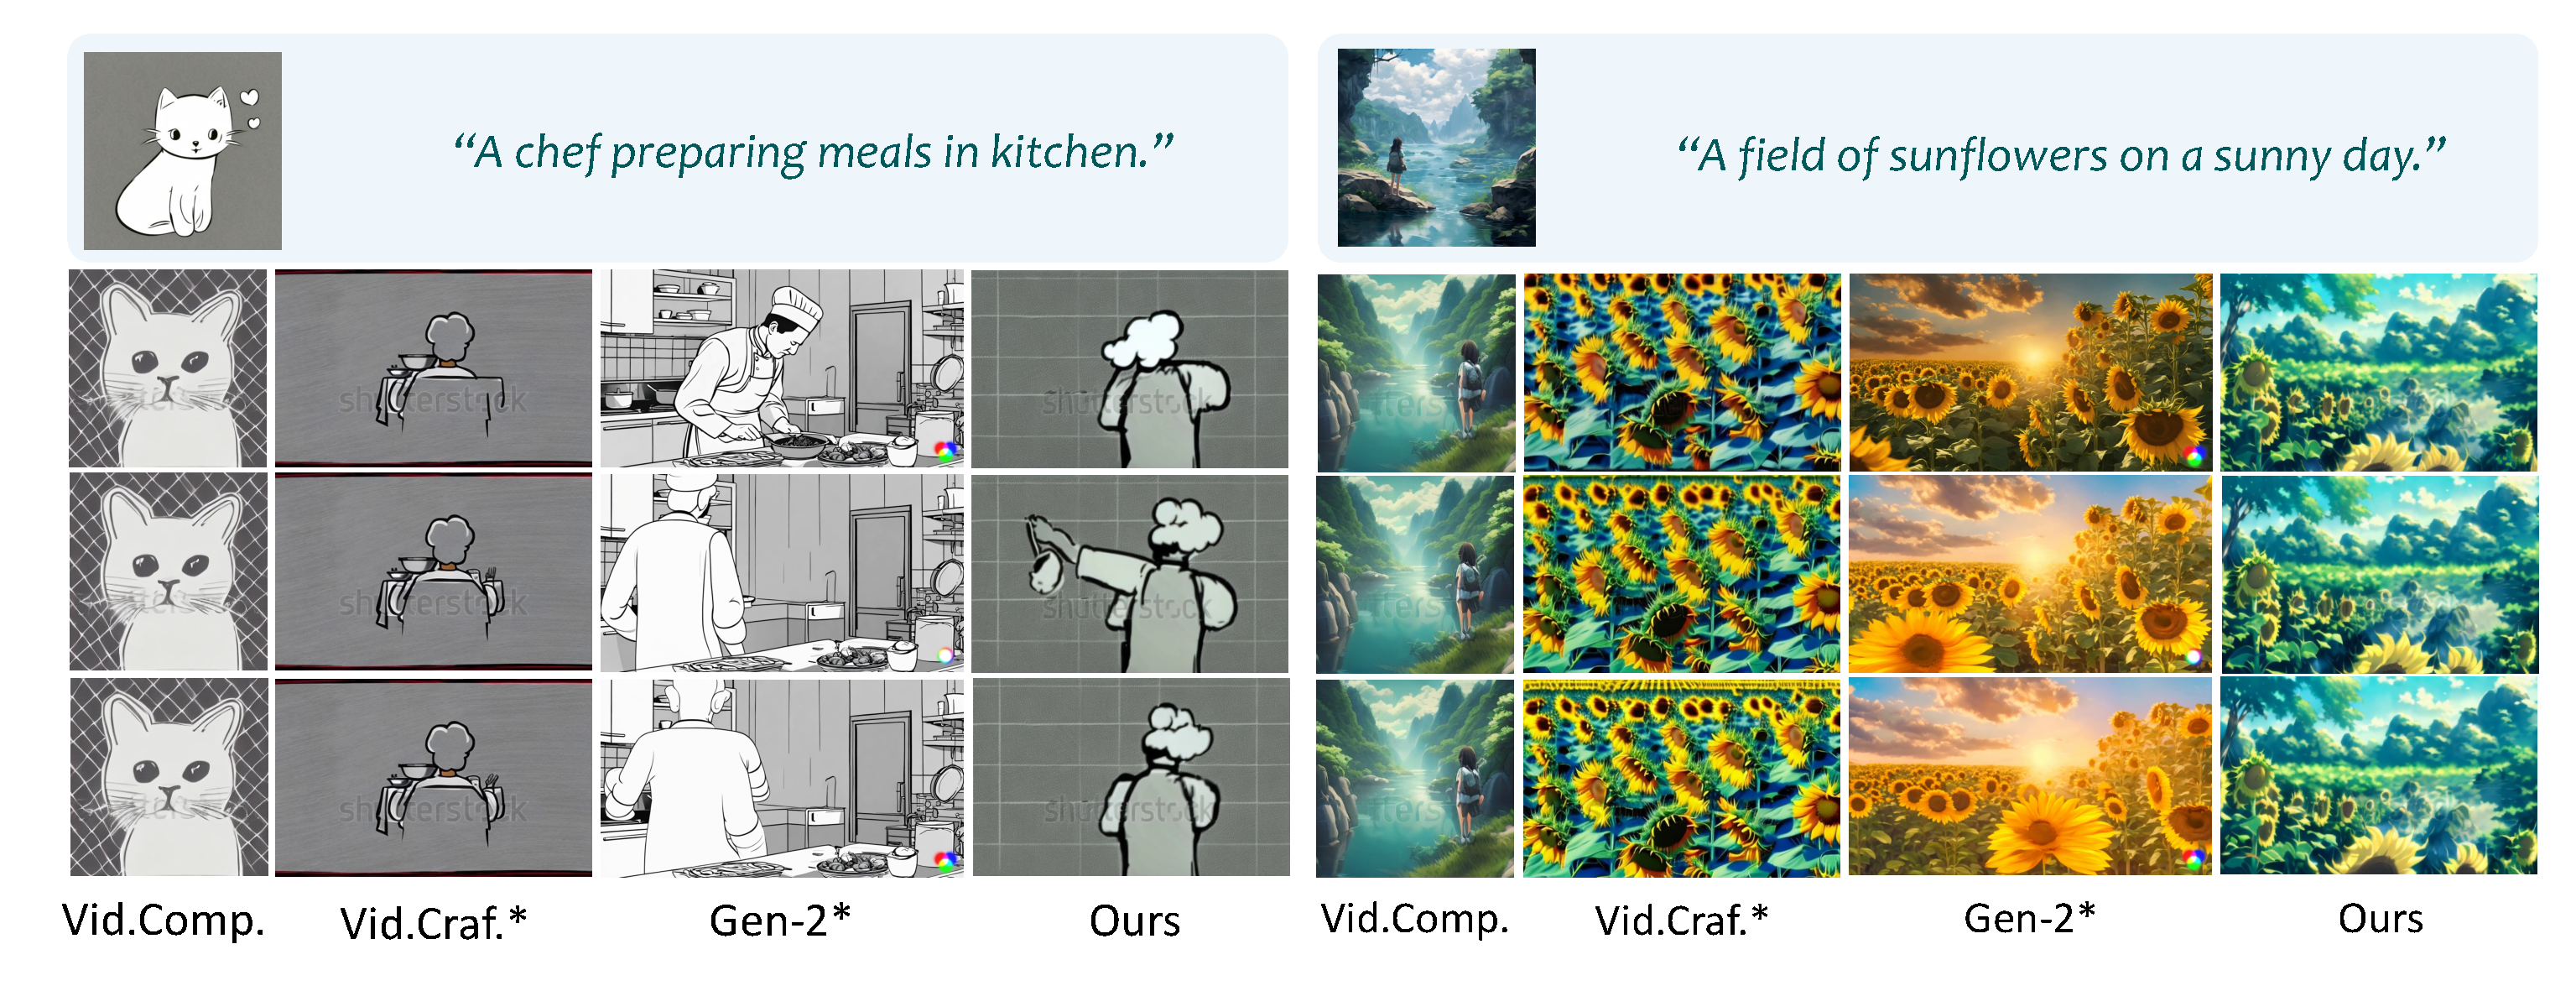
\includegraphics[width=0.9\linewidth]{figures/comp_video.pdf}\vspace{-1.5em}
    \caption{Visual comparison of single-reference guided T2V generation. Vid.Comp.: VideoComposer, Vid.Craf.: VideoCrafter
    %Our approach accurately captures the style of the reference image and generates videos that satisfy both text alignment and style conformity.
    } 
    \label{fig:result_video}
    \vspace{-1em}
\end{figure*}
%
\begin{figure*}[!h]
    \centering
    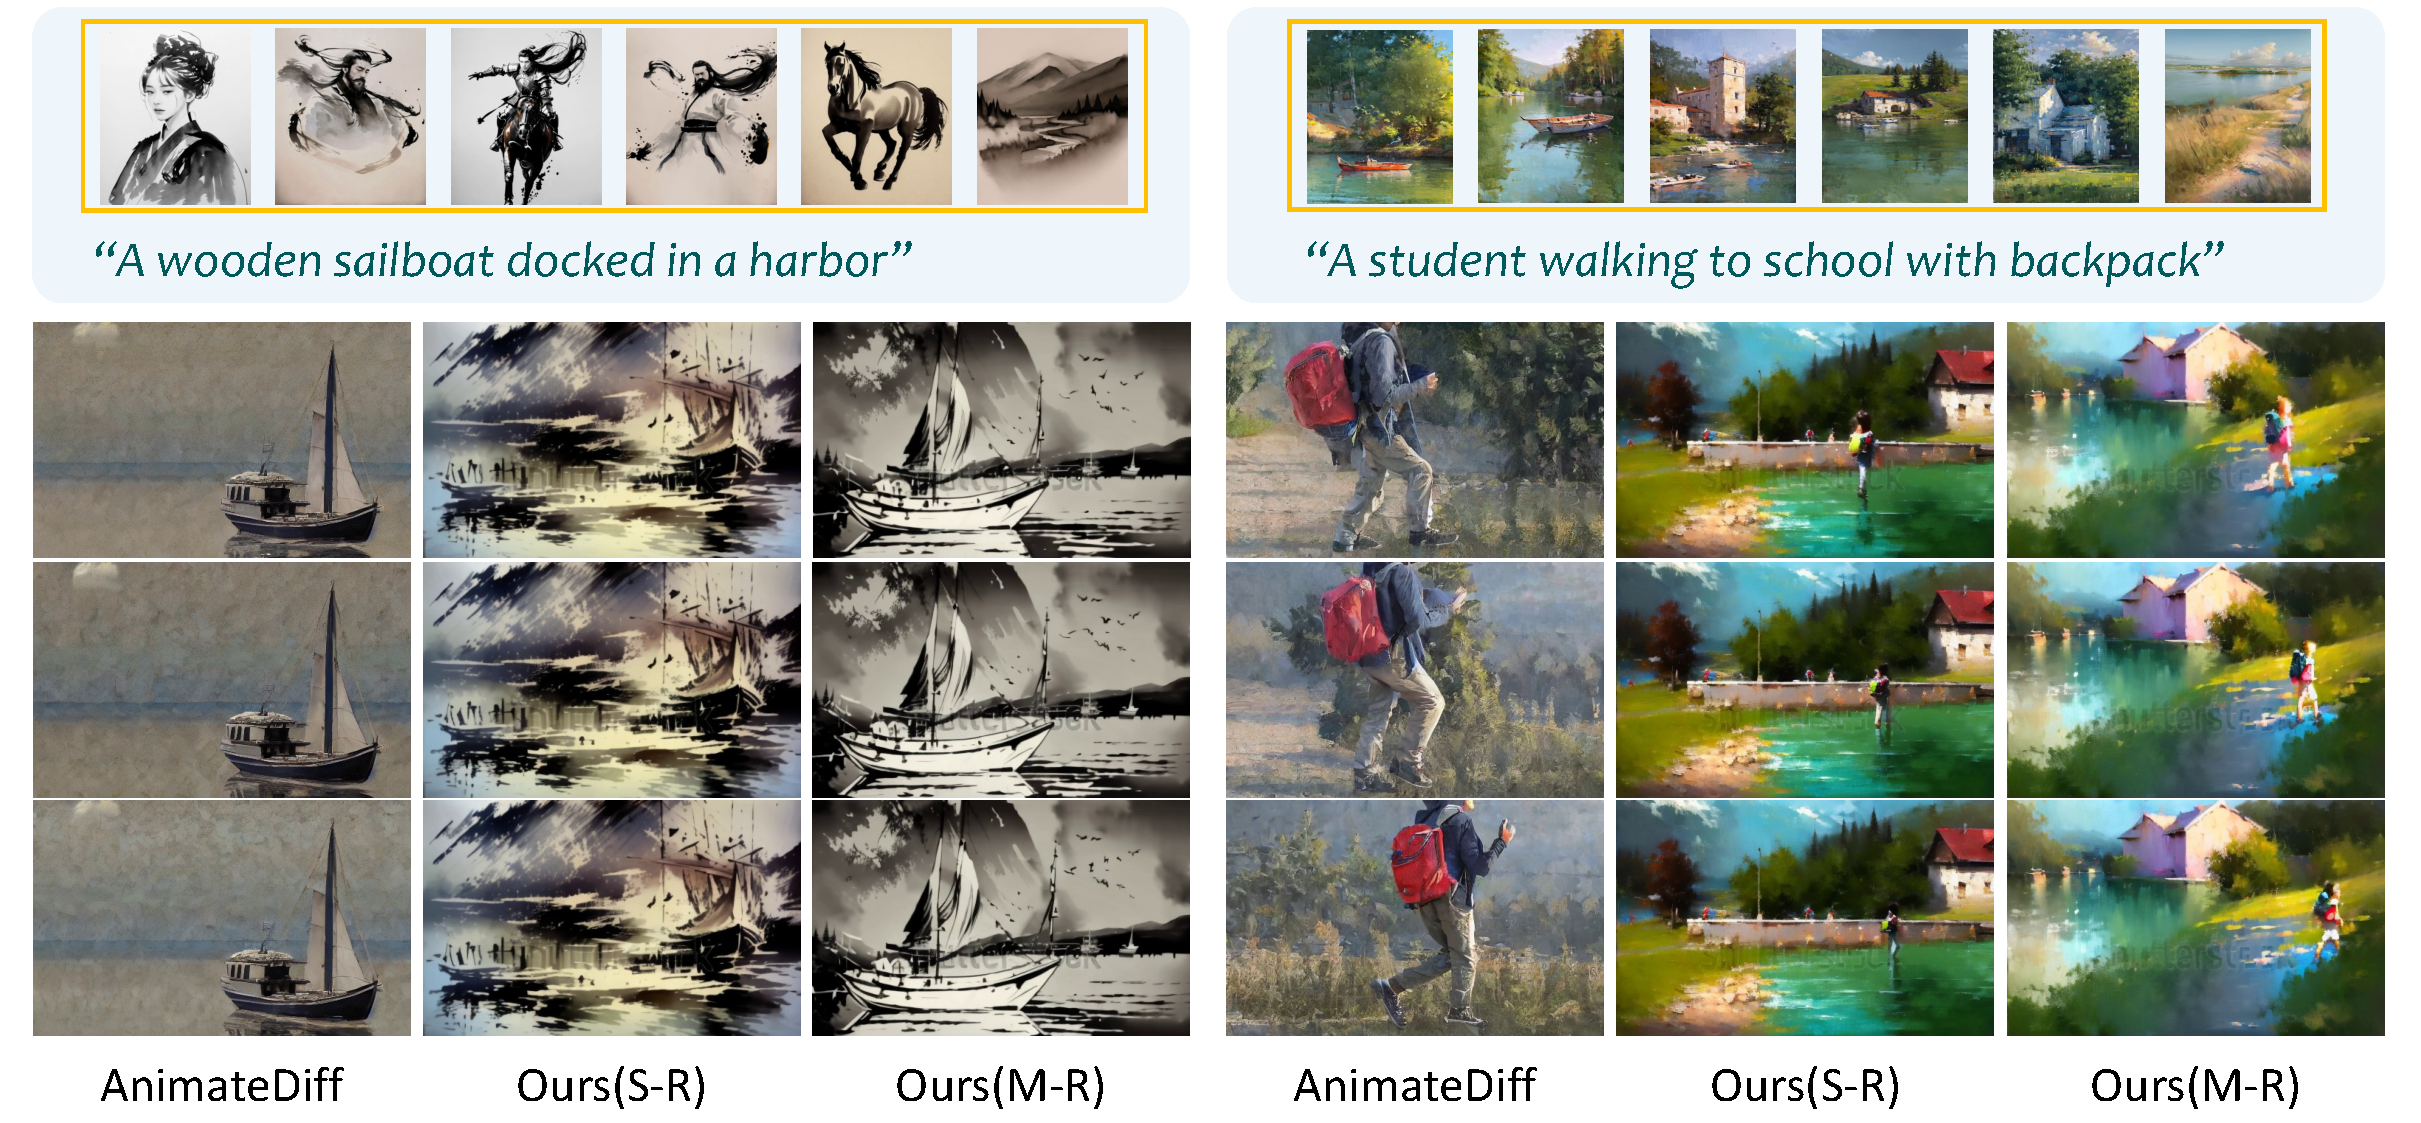
\includegraphics[width=0.87\linewidth]{figures/comp_video2.pdf}
    \vspace{-1em}
    \caption{Qualitative comparison of multi-reference style-guided T2V generation. S-R: Single-Reference, M-R: Multi-Reference
    %AnimateDiff tends to generate close-to-reamlism results despite the style references are typical artistic styles. In contrast, our approach performs better in text alignment, style conformity and temporal consistency.
    } 
    \vspace{-1em}
    \label{fig:result_multi_ref}
\end{figure*}



\begin{table}[!t]
\centering
\caption{Quantitative comparison of style-guided T2V generation. Top 3 rows: single-reference based gudiance. Bottom 3 rows: multi-reference based guidance. S-R: Single-Refernce, M-R: Multi-Reference, W.E.: Warping Errors.}
\label{tab:video_quan_clip}
\vspace{-1em}
\resizebox{\linewidth}{!}{
% \scriptsize
% \renewcommand\arraystretch{1.2}
\begin{tabular}{c c c cc} % {@{}lc@{}}
    % \toprule
    \toprule
    \multirow{2}{*}{Methods} & \multirow{2}{*}{CLIP-Text $\uparrow$} & \multirow{2}{*}{CLIP-Style $\uparrow$} & \multicolumn{2}{c}{Temporal Consistency} \\
    \cmidrule(lr){4-5}
      & & &
     ~CLIP-Temp $\uparrow$~ & \makecell{W.E.($\times10^{-3}$) $\downarrow$}\\
    \midrule
    VideoComposer & 0.0468 & \textbf{0.7306} & 0.9853 & \textbf{9.903} \\
    VideoCrafter* & 0.2209 & 0.3124 & 0.9757 & 61.41 \\
    Ours & \textbf{0.2726} & 0.4531 & \textbf{0.9892} & 18.73 \\
    \midrule
    ~AnimateDiff & \textbf{0.2867} & 0.3528 & 0.8903 & 37.17 \\
    Ours(S-R) & 0.2661 & 0.4803 & 0.9851 & 14.13 \\
    Ours(M-R) & 0.2634 & \textbf{0.4887} &\textbf{0.9852} & \textbf{9.396} \\
    \bottomrule
  \end{tabular}
}
\end{table}

\begin{table}[!t]
\centering

\caption{User study statistics of the selection rate for text alignment(\texttt{Text}), and preference rate for style conformity(\texttt{Style}) and temporal quality(\texttt{Temporal}). Top 3 rows: single-reference based guidance. Bottom 2 rows: multi-reference based guidance.}
\label{tab:video_quan_multi_ref}
\vspace{-1em}

\small
\begin{tabular}{c c c c} % {@{}lc@{}}
    % \toprule
    \toprule
    Methods & \texttt{Text} $\uparrow$ & \texttt{Style} $\uparrow$ & \texttt{Temporal} $\uparrow$ \\
    \midrule
    VideoCrafter* & 0.391 & 8.0\% & 4.4\%  \\
    Gen-2* & 0.747 & 23.1\% & 51.1\% \\
    Ours & 0.844 & 68.9\% & 44.4\% \\
    \midrule
    ~AnimateDiff~ & 0.647 & 10.0\% & 19.3\% \\
    Ours(M-R) & 0.907 & 90.0\% & 80.7\% \\
    \bottomrule
\end{tabular}
\end{table}

Existing approaches for style-guided video generation can be divided into two categories: one is the single-reference based methods that are usually tuning-free, e.g. VideoComposer~\cite{wang2024videocomposer}; the other is the multi-reference based methods that generally requires multiple references for fine-tuning, e.g. AnimateDiff~\cite{guo2023animatediff}. We make comparisons with these methods, respectively. 
% Apart from the quality metrics, we further conduct user study to evaluate the stylized video results, including text alignment, style conformity and temporal quality.


\vspace{-0.5em}
\paragraph{Single-Reference based Guidance.}VideoComposer~\cite{wang2024videocomposer} is a controllable video generation model that allows multiple conditional inputs including style reference image. It is a natural competitor of our method. 
Besides, we construct two additional comparative methods, i.e. VideoCrafter* and Gen2*, which extend VideoCrafter~\cite{chen2023videocrafter} and Gen2~\cite{Gen-2}, the state-of-the-art T2V models in open-source and close-source channels respectively, to make use of style reference images by utilizing GPT-4V~\cite{openai2023gpt4v} to generate style prompts from them.
% The evaluation is conducted on 240 text-style pairs, as introduced in Sec.~\ref{sec:test_dataset}. 
The quantitative comparison is tabulated in Table~\ref{tab:video_quan_clip}. Several typical visual examples are illustrated in Figure~\ref{fig:result_video}.

We can observe that: 
(i) VideoComposer tends to copy content from style references and struggles to generate text-aligned content, which is possibly because of the invalid decoupling learning. Consequently, its results exhibit abnormally high style conformity and very low text alignment. In addition, VideoComposer often generates static videos, thus having the lowest warping errors, but this does not mean that their results perform best in temporal quality. 
(ii) VideoCrafter* exhibits limited stylized generation capabilities, producing videos with diminished style and disjointed movements. Gen-2* demonstrates superior stylized generation capabilities. However, Gen-2 is still limited by the inadequate representation of style in textual descriptions, and is more prone to sudden changes in color and luminance. (iii) In comparison, our method captures styles more effectively and reproduces them in the generated results.

\begin{figure}[!t]
    \centering
    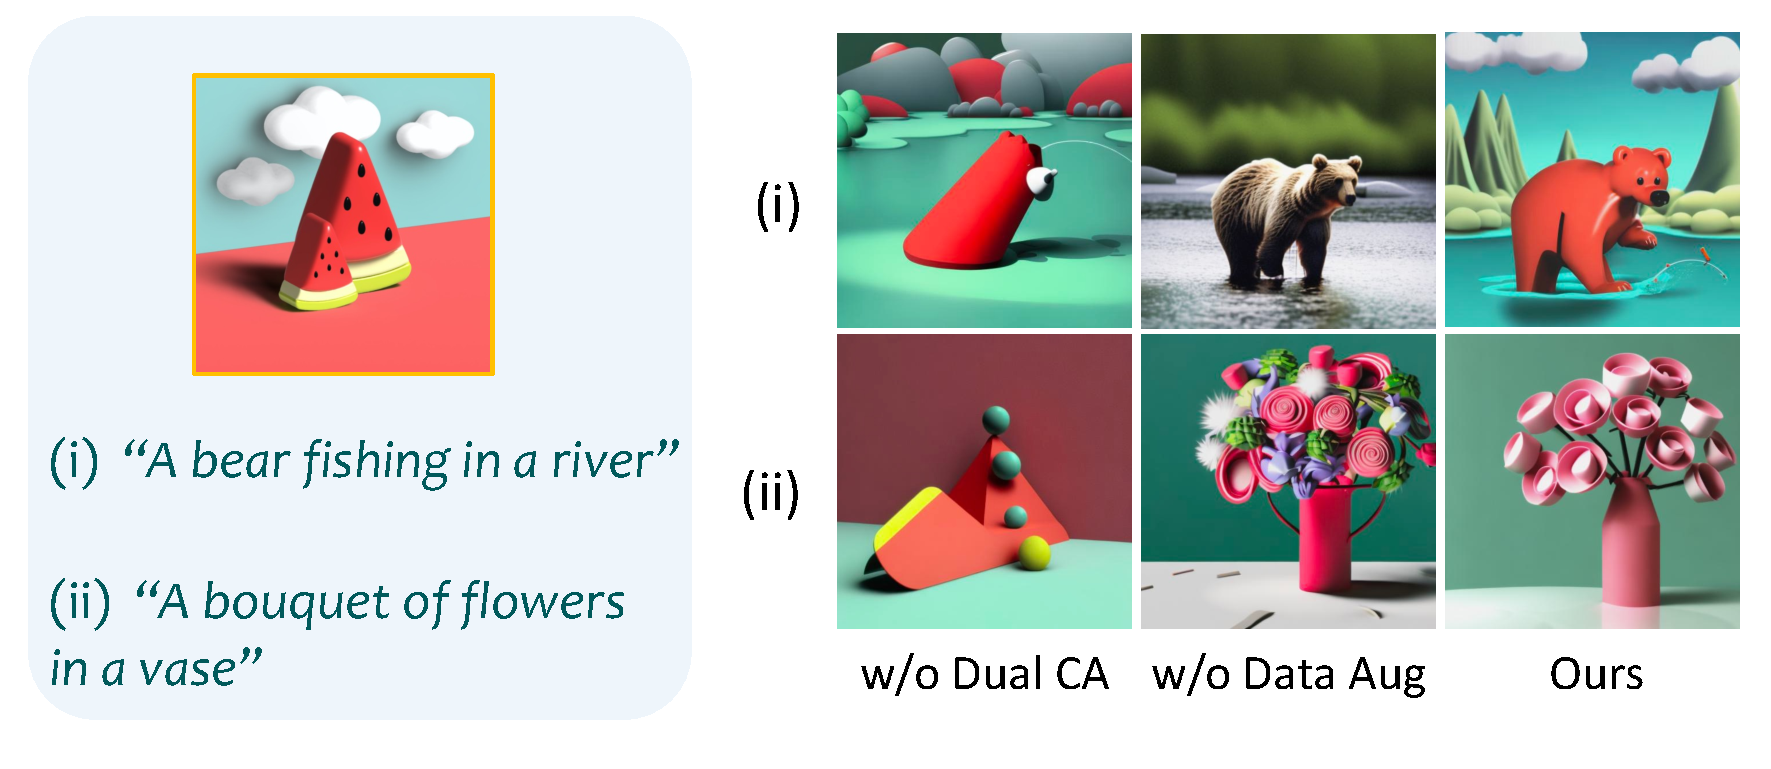
\includegraphics[width=\linewidth]{figures/ablation_img_1.pdf}
    \vspace{-3em}
    \caption{Effects of dual cross-attention and data augmentation.} 
    \label{fig:ablation_img_1_2}
    \vspace{-1em}
\end{figure}


\vspace{-0.5em}
\paragraph{Multi-Reference based Guidance.}
AnimateDiff~\cite{guo2023animatediff} denotes a paradigm to turn personalized SD (i.e., SD fine-tuned on specific-domain images via LoRA~\cite{hu2022lora} or Dreambooth~\cite{dreambooth}) for video generation, namely combined with pre-trained temporal blocks of T2V models. It can generate very impressive results if the personalized SD is carefully prepared, however, we find it struggle to achieve as satisfactory results if only a handful of style reference images are available for training.
We conduct an evaluation on 60 text-style pairs with multi-references, as presented in Sec.~\ref{sec:test_dataset}. We train Dreambooth~\cite{dreambooth} models for each style and incorporate them into AnimateDiff based on their released codebase. Thanks to the flexibility of Q-Former, our method also supports multiple reference images in a tuning-free fashion, i.e. computing the image embeddings of each reference image and concatenating all embeddings as input to the Q-Former.
Results are compared in Table~\ref{tab:video_quan_multi_ref} and Figure~\ref{fig:result_multi_ref} respectively.

According to the results, AnimateDiff struggles to achieve high-fidelity stylistic appearance while tends to generate close-to-realism results despite the style references are typical artistic styles. In addition, it is vulnerable to temporal artifacts. As the trained personalized-SD can generate decent stylistic images (provided in the supplementary materials), we conjecture that the performance degradation is caused by the incompatibility from the pre-trained temporal blocks and independently trained personalized-SD models, which not only interrupts temporal consistency but also weakens the stylistic effect.
In contrast, our method can generate temporal consistent videos with high style conformity to the reference images and accurate content alignment with the text prompts. Furthermore, using multiple references can further promote the performance, which offers additional advantages in practical applications.


%---------------------------------
\subsection{Ablation Study}
\label{subsec:ablation}
%---------------------------------

\begin{figure}[!t]
    \centering
    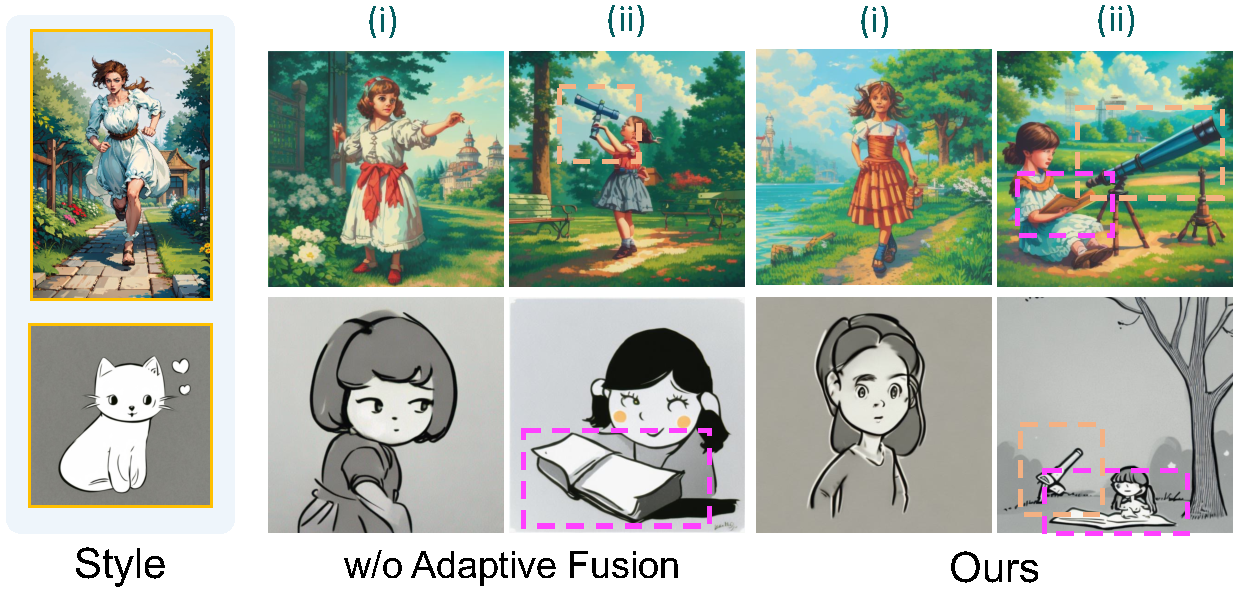
\includegraphics[width=\linewidth]{figures/ablation_no_scale.pdf
    }
    \vspace{-2em}
    \caption{Effect of adaptive content-style fusion. It shows superiority in generalization to extreme cases, e.g. long text description. Two text prompts are used: (i) A little girl; (ii) \textit{A little girl \textcolor[RGB]{255, 64, 255}{reading a book} in the park, with \textcolor[RGB]{244, 177, 131}{a telescope} nearby pointed at the sky}.}
    \label{fig:ablation_no_fusion}
    \vspace{-0.7em}
\end{figure}

% We make ablation studies on some important designs of our method, including data augmentation, module architectures, and training strategies, to validate their effectiveness.

\paragraph{Data Augmentation.}
We first study the effectiveness of content-style decoupled data augmentation. As depicted in Table~\ref{tab:ablation_img}, training with the original image-caption pairs restricts the model's ability to extract style representations, leading to lower style conformity. For example, as shown in Figure~\ref{fig:ablation_img_1_2}, method without data augmentation fails to capture the "3D render" style from the reference.


\paragraph{Dual Cross-Attention.} 
As discussed in Sec.~\ref{subsec:style_modulation},  we make a comparison between \textit{attach-to-text} and \textbf{dual cross-attention} to study their effects. Results are presented in Table ~\ref{tab:ablation_img} and Figure~\ref{fig:ablation_img_1_2}, revealing that \textit{attach-to-text} tends to directly fuse the content from the reference image and the text prompts rather than combining the text-based content and image-based style. This indicates the effectiveness of \textbf{dual cross-attention} in facilitating content-style decoupling.


\paragraph{Adaptive Style-Content Fusion.}
As previously discussed in Figure~\ref{fig:scale_factor_viz}, our proposed adaptive style-content fusion module demonstrates effectiveness in adaptively processing various conditional contexts. It benefits the generalization ability of model to deal with diverse combinations of content prompt and style image. Figure~\ref{fig:ablation_no_fusion} reveals that although the baseline can handle easy prompt inputs like "A little girl", it struggles to accurately generate all objects described in longer prompts. In contrast, the adaptive fusion module can achieve decent text alignment for long text descriptions thanks to its flexibility to adaptive balance between content and style.

\paragraph{Two-Stage Training Scheme.}
Our proposed training scheme consists of two stages, i.e., style adapter training and temporal adaption. To show its necessity, we build two baselines: (i) \textit{w/o Temporal Adaption}: that we train a style adapter on image data and apply it directly to stylized video generation without finetuning; (ii) \textit{joint training}: that we conduct style adapter training and temporal blocks finetuning on image-video dataset simultaneously.
As depicted in Table~\ref{tab:ablation_video}, baseline (i) exhibits inferior temporal consistency when applied directly to video, and undermines the content alignment and style conformity. As for baseline (ii), the learning of style embedding extraction seems to be interfered by the joint finetuning of temporal blocks, which impedes it to generate desirable stylized videos.


\begin{table}[!t]
\centering

\caption{Ablation studies on style modulation designs. The performance is evaluated based on the style-guided T2I generation.}
\label{tab:ablation_img}
\vspace{-1em}
    
\small
% \renewcommand\arraystretch{1.2}
  \begin{tabular}{ccc} % {@{}lc@{}}
    % \toprule
    \hline
    Methods & \texttt{CLIP-Text} $\uparrow$ & \texttt{CLIP-Style} $\uparrow$ \\
    \hline
    Ours & 0.3028 & 0.4836 \\
    ~w/o Data Augmentation & 0.3173 & 0.4005 \\
    w/o Dual Cross Attention & 0.0983 & 0.7332 \\
    w/o Adaptive Fusion & 0.2807 & 0.4925 \\
    \hline
  \end{tabular}
\vspace{-1em}
\end{table}


\begin{table}[!t]
\centering
\vspace{1em}

\caption{Ablation study on our two-stage training scheme.}
\vspace{-1em}
\label{tab:ablation_video}
% \renewcommand\arraystretch{1.5}
\resizebox{\linewidth}{!}{

\begin{tabular}{c c c cc} % {@{}lc@{}}
    % \toprule
    \toprule
    \multirow{2}{*}{Methods} & \multirow{2}{*}{CLIP-Text $\uparrow$} & \multirow{2}{*}{CLIP-Style $\uparrow$} & \multicolumn{2}{c}{Temporal Consistency} \\
    \cmidrule(lr){4-5}
      & & &
     ~CLIP-Temp $\uparrow$~ & \makecell{W.E.($\times10^{-3}$) $\downarrow$}\\
    \midrule
    w/o Temporal Adaption  & 0.2691 & 0.3923 & 0.9612 & 47.88 \\
    Joint Training & 0.3138 & 0.2226 & 0.9741 & 24.74 \\
    Two-Stage(ours) & \textbf{0.2726} & \textbf{0.4531} & \textbf{0.9892} & \textbf{18.73} \\
    \bottomrule
  \end{tabular}
}

    \vspace{-1em}
  
\end{table}

%
% \begin{figure}[!t]
%     \centering
%     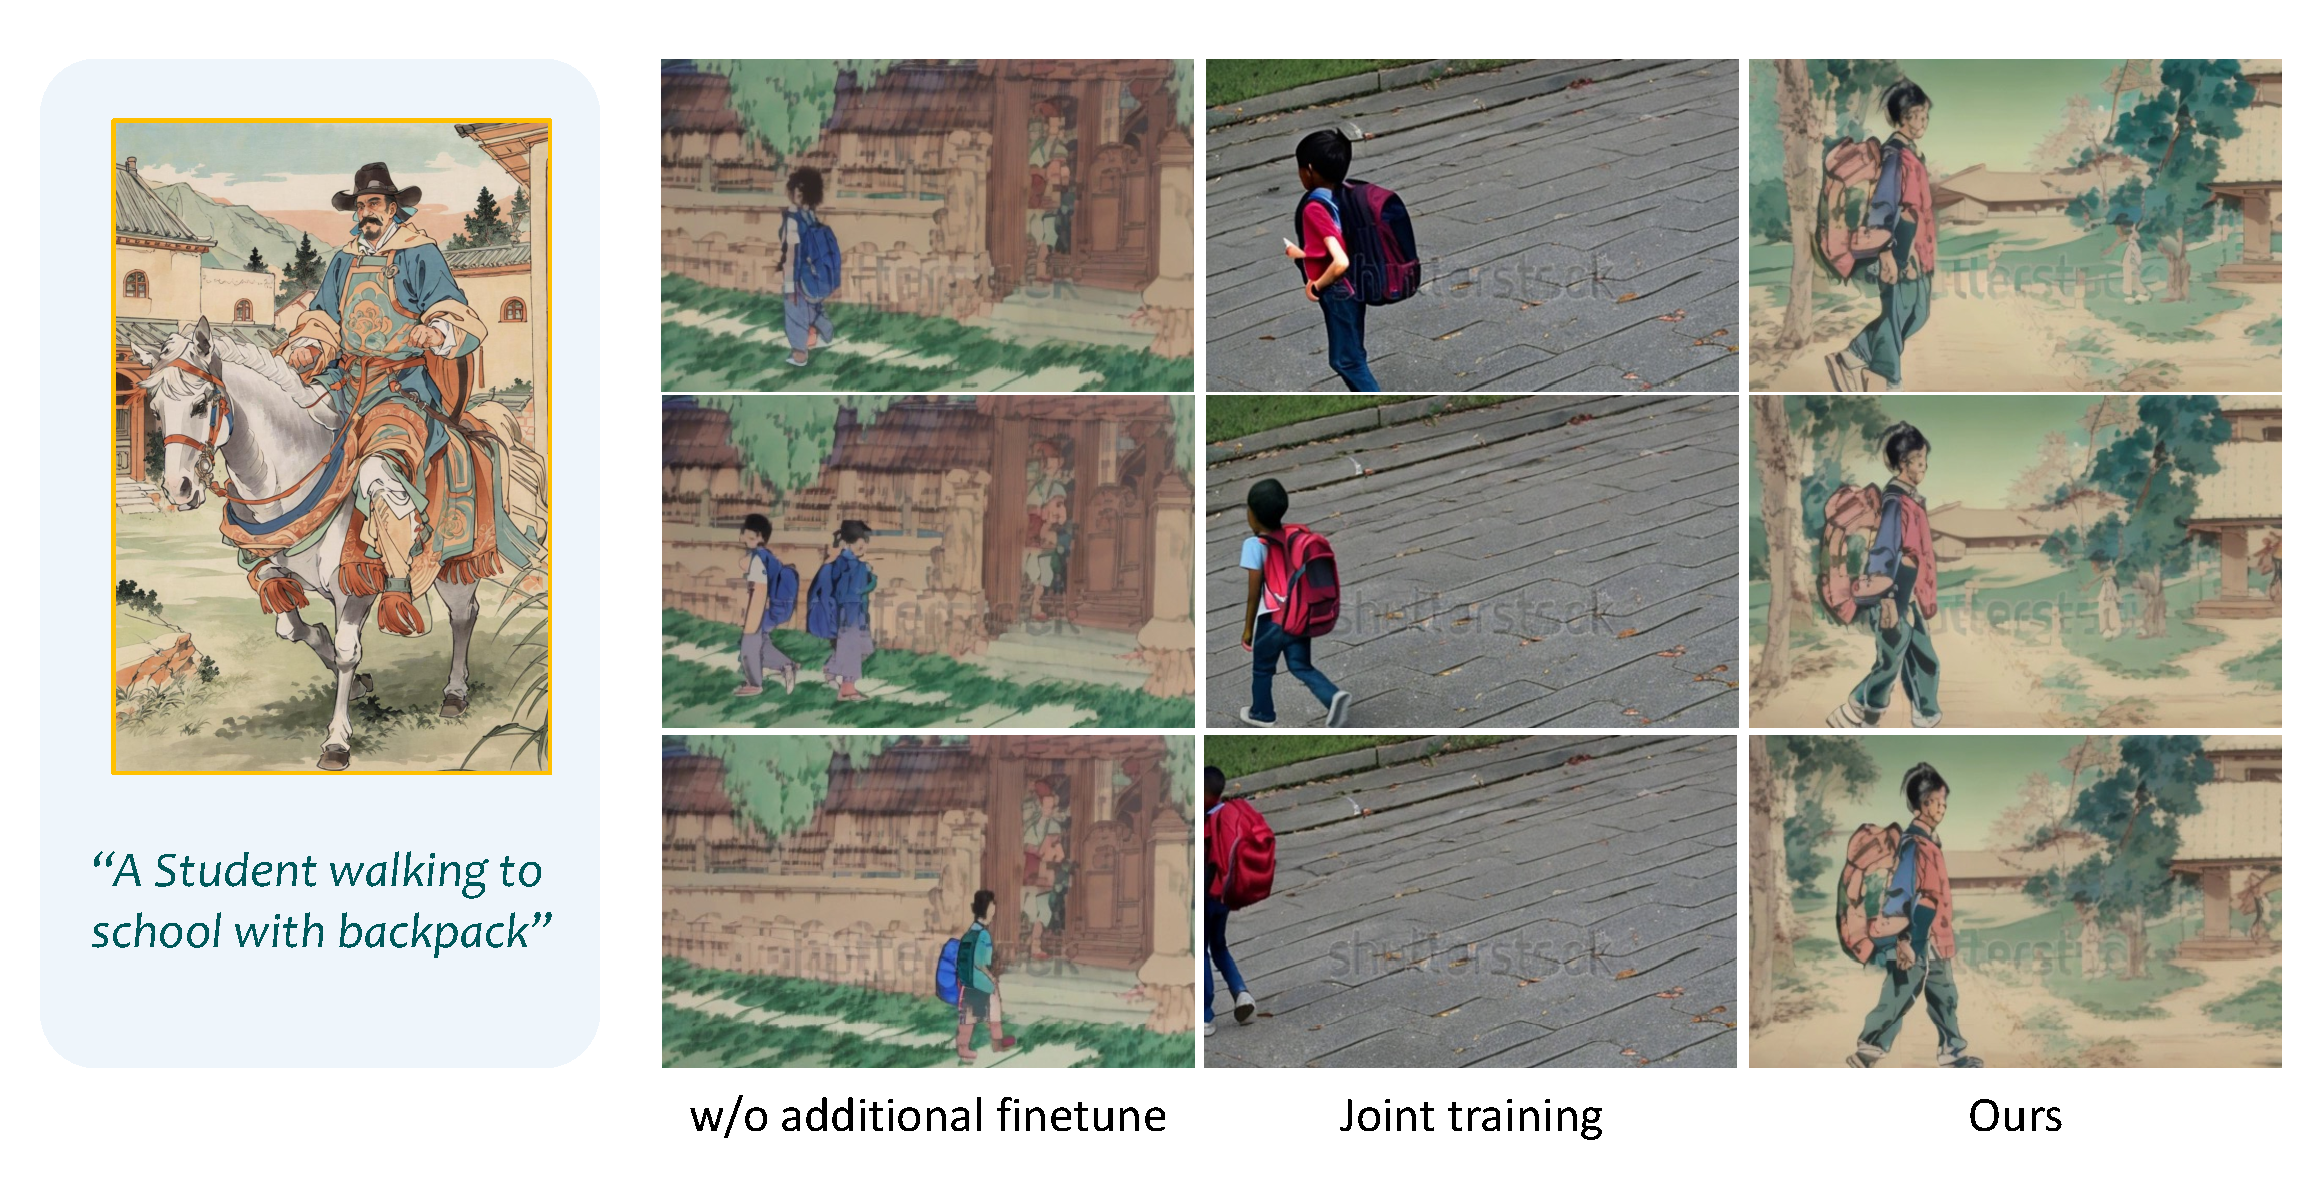
\includegraphics[width=\linewidth]{figures/ablation_two_stage.pdf}
%     \vspace{-2em}
%     \caption{Comparison on the effects of different training schemes.}
%     \label{fig:ablation_two_stage}
%     \vspace{-1em}
% \end{figure}



\section{Conclusion}

We have explored the direct application of Transformers to image recognition.
Unlike prior works using self-attention in computer vision, we do not introduce image-specific inductive biases into the architecture apart from the initial patch extraction step.
Instead, we interpret an image as a sequence of patches and process it by a standard Transformer encoder as used in NLP.
This simple, yet scalable, strategy works surprisingly well when coupled with pre-training on large datasets.
Thus, \oursfull matches or exceeds the state of the art on many image classification datasets, whilst being relatively cheap to pre-train.

While these initial results are encouraging, many challenges remain.
One is to apply \oursabbrv to other computer vision tasks, such as detection and segmentation.
Our results, coupled with those in \citet{carion20-detr}, indicate the promise of this approach.
Another challenge is to continue exploring self-supervised pre-training methods.
Our initial experiments show improvement from self-supervised pre-training, but there is still large gap between self-supervised and large-scale supervised pre-training.
Finally, further scaling of \oursabbrv{} would likely lead to improved performance.

\citestyle{acmauthoryear}
\bibliographystyle{ACM-Reference-Format}
\bibliography{reference}

\clearpage

\newpage
\appendix
\section*{Appendix}
In support of the main paper,~\cref{app:proofs} presents the proofs for the propositions in the paper,~\cref{app:additional_findings} includes additional findings that support our main results, and~\cref{app:further_discussion} provides further discussion on conditions that lead to grokking.
\section{Proofs}\label{app:proofs}
\begin{proof}[Proof of~\cref{prop:stablemax}]
\begin{align}
    \softmax\left(g\left(x_i\right)\right) &= \frac{e^{g(x_i)}}{\sum_j e^{g(x_j)}}\\
    &= \begin{cases}
\frac{e^{\log(x_i+1)}}{\sum_j e^{\log(x_j+1)}} & \text{if } x_i \geq 0, \\
\frac{e^{-\log(-x_i+1)}}{\sum_j e^{-\log(-x_j+1)}} & \text{if } x_i < 0
\end{cases}\\
&= \begin{cases}
\frac{x_i+1}{\sum_j x_j+1} & \text{if } x_i \geq 0, \\
\frac{\frac{1}{-x_i+1}}{\sum_j \frac{1}{-x_j+1}} & \text{if } x_i < 0
\end{cases}\\
&= \stablemax(x_i).
\end{align}
\end{proof}

\begin{proof}[Proof of~\cref{prop:NLMGrad}]
To prove that any nonzero $-\nabla_{\perp} \loss(\bm{\theta}_t)$ is a descent direction, we need to show that $\left\langle -\nabla_{\perp} \loss(\bm{\theta}_t), \nabla\loss(\bm{\theta}_t) \right\rangle < 0$, assuming $\nabla_{\perp} \loss(\bm{\theta}_t) \neq \mathbf{0}$:
    \begin{equation}
        \left\langle \nabla\loss(\bm{\theta}_t), -\nabla\loss(\bm{\theta}_t) + \left( \frac{\bm{\theta}_t^\top \nabla \loss(\bm{\theta}_t)}{\bm{\theta}_t^\top \bm{\theta}_t} \right)\bm{\theta}_t  \right\rangle \leq 0.
    \end{equation}
    Expanding this yields:
    \begin{align}
        -\left\|\nabla\loss(\bm{\theta}_t)\right\|^2_2 + 
        \left\langle  \nabla\loss(\bm{\theta}_t), \bm{\theta}_t \frac{\bm{\theta}_t^\top \nabla \loss(\bm{\theta}_t)}{\bm{\theta}_t^\top \bm{\theta}_t}\right\rangle
        &\leq 0.
    \end{align}
    Since the inequality is unaffected by the scaling of the left hand side, we can, without loss of generality, assume that the gradients are normalized, leading to:
    \begin{align}\label{eq:incidence}
        \left\langle \nabla\loss(\bm{\theta}_t), \bm{\theta}_t \frac{\bm{\theta}_t^\top \nabla \loss(\bm{\theta}_t)}{\bm{\theta}_t^\top \bm{\theta}_t}\right\rangle
        &{\leq} 1.
    \end{align}
    Since $\bm{\theta}_t \frac{\bm{\theta}_t^\top \nabla \loss(\bm{\theta}_t)}{\bm{\theta}_t^\top \bm{\theta}_t}$ denotes the projection of the gradient onto the space spanned by the weights, $\langle\cdot,\cdot\rangle$ will measure the acute angle of incidence and hence~\cref{eq:incidence} holds, with equality iff $\nabla_{\perp} \loss(\bm{\theta}_t) = \mathbf{0}$, which is prevented by assumption. This proves that $-\nabla_{\perp} \loss(\bm{\theta}_t)$ is a descent direction while being perpendicular to the weights. %, the angle between $\loss(\bm{\theta}_t)$ and this projection will be the acute .
\end{proof}
We note that the \ograd stops when $\nabla_{\perp}\loss(\bm{\theta}_t) = \mathbf{0}$. If $\nabla\loss(\bm{\theta}_t) \neq \mathbf{0}$, this corresponds to the condition where the gradient is in the same direction with the parameter vector. $\nabla_{\perp}\loss(\bm{\theta}_t) = \mathbf{0}$ can also be the case if $\nabla\loss(\bm{\theta}_t) = \mathbf{0}$, which corresponds to the loss function being at a local optimum.

\section{Additional Findings}\label{app:additional_findings}


\subsection{Further evidence that SC prevents grokking} \label{app:sc_intervention}
\begin{wrapfigure}[12]{R}{0.38\textwidth}
            \vspace{-0.4cm}
            \begin{center}
    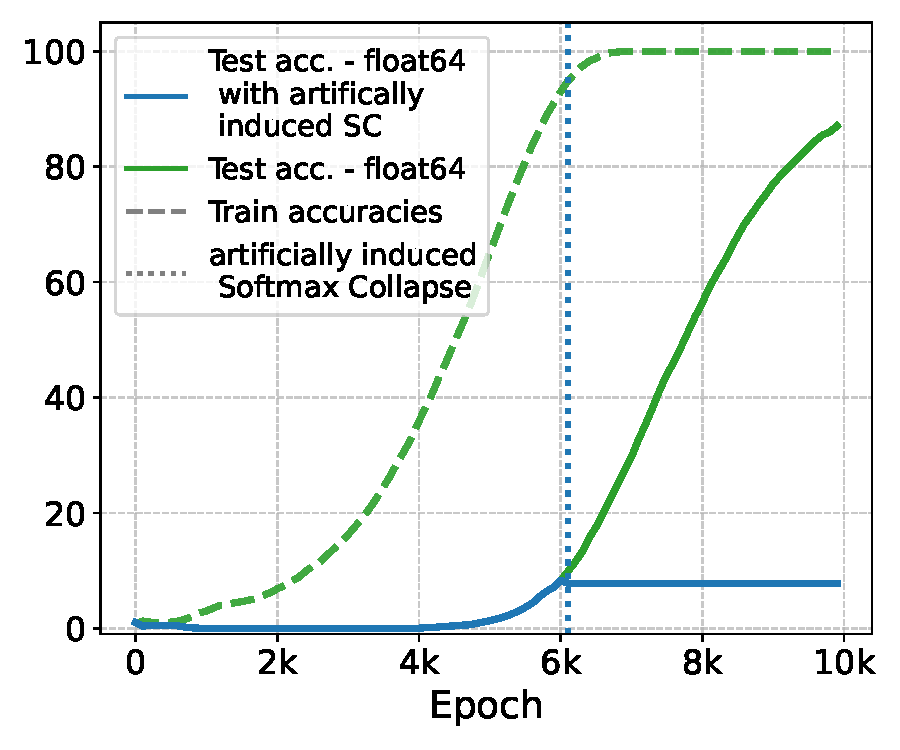
\includegraphics[width=\linewidth]{grokking_iclr_arxiv/figures/artificially_induced_sc.pdf}
            \end{center}
            \vspace{-12pt}
            \caption{Taking a model that would normally generalize (green) and artificially inducing SC has a very similar effect to the one observed in \cref{fig:grokking_stops}.\vspace{4mm}}
    \label{fig:sc_intervention}
\end{wrapfigure} 
While SC leads the gradient from correctly predicted samples to be zero, it does not do this for the incorrect classes. To validate that setting the gradients from the correct classes to zero is enough to stop learning, we do this artificially for a model that is generalizing and show that learning stops after this intervention. In \cref{fig:sc_intervention} we see that the baseline model shown in geen generalizes, but this is stopped at epoch 6000 for the model shown in blue, after we perform this intervention.

The intervention is implemented by multiplying the logits for the right classes by 0 at each step after epoch 6000.

\begin{comment}
\begin{figure}[h]
    \centering
    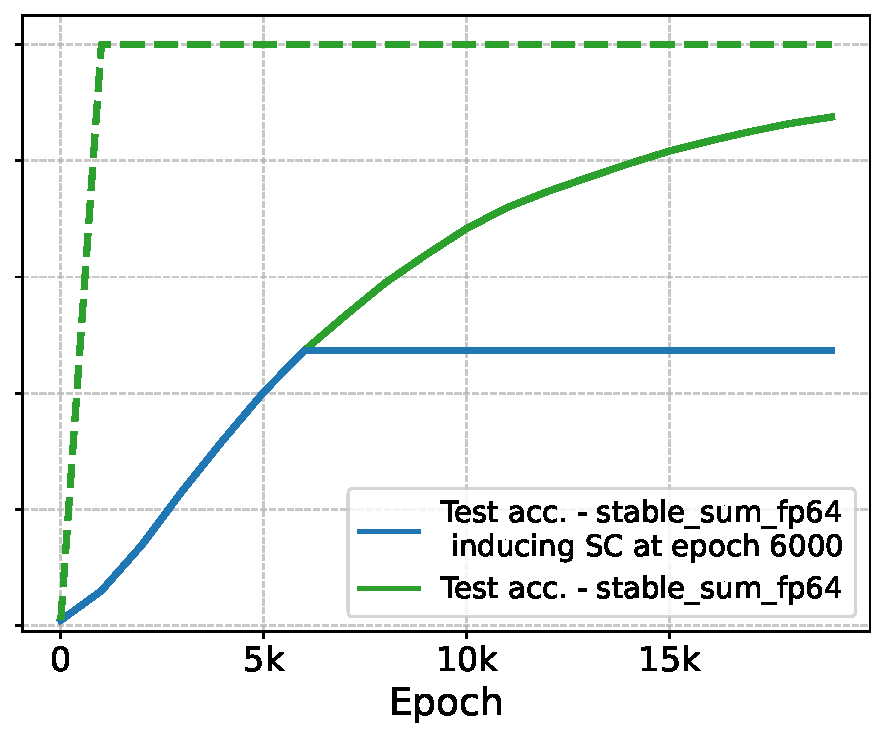
\includegraphics[width=0.5\linewidth]{grokking_iclr/figures/sc_intervention.pdf}
    \caption{Taking a model that would normally generalize (green) and artificially inducing SC has a very similar effect to the one observed in \cref{fig:grokking_stops}}.
    \label{fig:sc_intervention}
\end{figure}    
\end{comment}


\subsection{SGD with learning rate scheduling}
To show that our results are not due to the inductive bias of adaptive moments in optimizers like AdamW, we replicate some of the AdamW results using SGD with a learning rate scheduler. Our scheduler is similar to the one in \cite{Lyu2019-sc} except at each step we divide the learning rate by the norm of the full gradient, instead of the loss. In \cref{fig:grokking_stops_lr_sch} we observe that SC also puts an end to grokking in this setting.
\vspace{5.75mm}\\

\begin{figure}[t]
\centering
\begin{subfigure}{.32\textwidth}
  \centering
  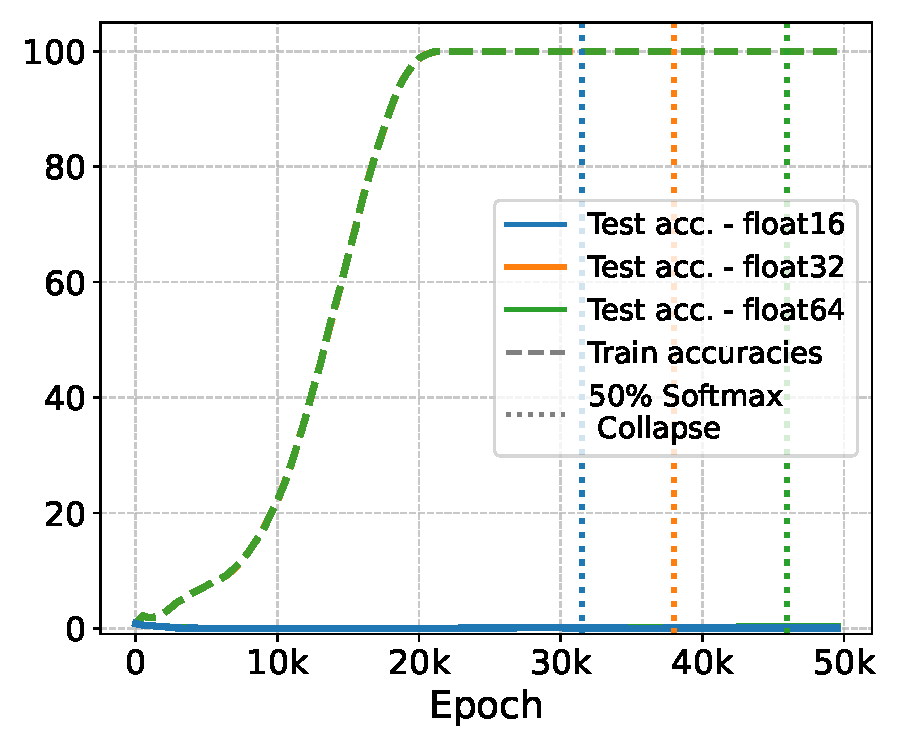
\includegraphics[width=\linewidth]{grokking_iclr_arxiv/figures/float32vsfloat64_40_percent_lr_sch.pdf}
  \caption{40\% training data}
  \label{fig:grokking_stops_40_lr_sch}
\end{subfigure}
\hfill
\begin{subfigure}{.32\textwidth}
  \centering
  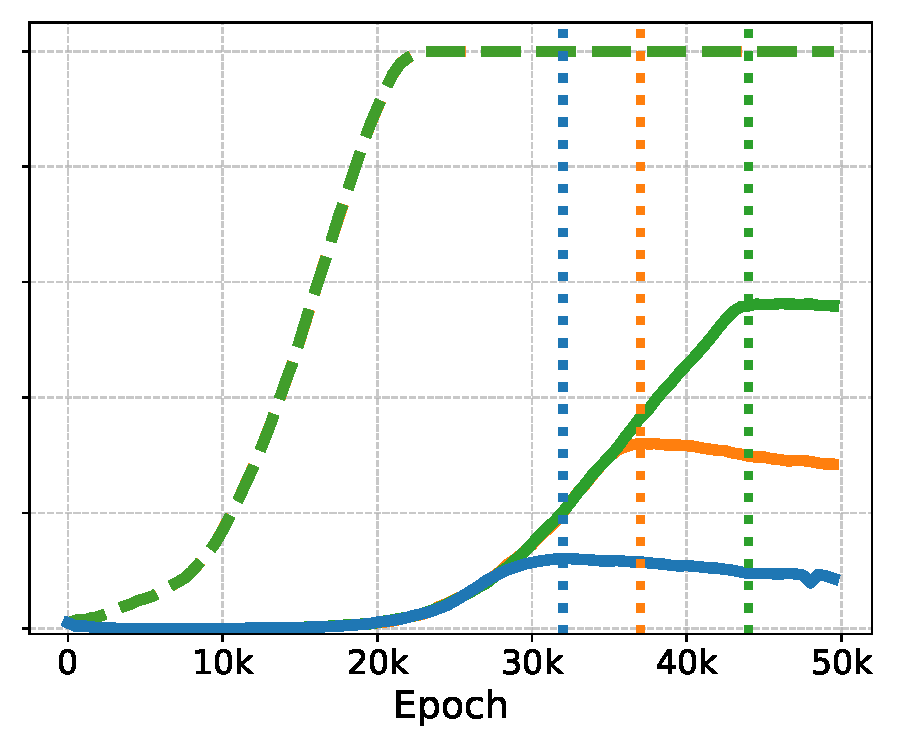
\includegraphics[width=\linewidth]{grokking_iclr_arxiv/figures/float32vsfloat64_60_percent_lr_sch.pdf}
  \caption{60\% training data}
  \label{fig:grokking_stops_60_lr_sch}
\end{subfigure}
\hfill
\begin{subfigure}{.32\textwidth}
  \centering
  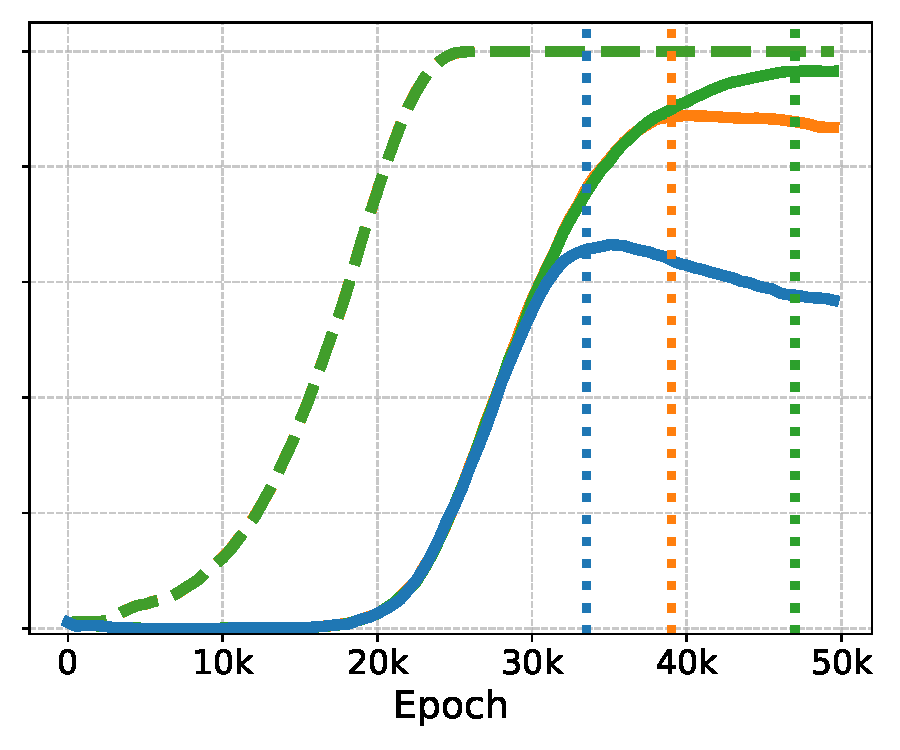
\includegraphics[width=\linewidth]{grokking_iclr_arxiv/figures/float32vsfloat64_70_percent_lr_sch.pdf}
  \caption{70\% training data}
\end{subfigure}
\caption{We show that the same dynamics observed in \cref{fig:grokking_stops} can be observed with a learning rate scheduler instead of AdamW. This shows that this is not due to an implicit bias of adaptive optimizers.}
\label{fig:grokking_stops_lr_sch}
\vspace{-5mm}
\end{figure}

\vspace{-5mm}
\section{Effective Learning Rate}
\begin{wrapfigure}[13]{R}{0.4\textwidth}
            \vspace{-1.2cm}
            \begin{center}
    \includegraphics[width=0.4\textwidth]{grokking_iclr_arxiv/figures/gradient_norms.pdf}
            \end{center}
            \vspace{-10pt}
            \caption{Gradient absorption errors during training on addition modulo 113.}
            \label{fig:gradient_absorption}
\end{wrapfigure} 
Unexplored in the main paper, NLM also has the effect of reducing the effective learning rate. For a gradient update using regular gradient descent $\bm{\theta}_{t+1} = \bm{\theta}_t - \eta \nabla \loss(\bm{\theta}_t)$ it is easy to see that $||\bm{\theta}_{t+1} - \bm{\theta}_{t}|| \to 0$ as $||\nabla \loss(\bm{\theta}_t)|| \to 0$. This problem has been observed before when training beyond the point of overfitting, for example, \cite{Lyu2019-sc} addressed it by using a loss based learning rate scheduler to keep up with the gradient. Theoretically, an alternative could be to simply extend the duration of training. According to our hypothesis, training for long enough should eventually lead to generalization on grokking tasks if we prevent SC. However, we find that another kind of floating point error can also appears in these settings, namely, gradient absorption errors in the weights. 

For a weight $w$, gradient absorption errors happen when a gradient update is small enough that it leaves the weight unchanged. Using the notation outlined in this paper this can be formalised as $w -\eta \frac{\partial \mathcal{L}}{\partial w} \doteq w$. In \cref{fig:gradient_absorption} we show that this happens for an MLP trained with SGD on modular addition using 30\% of the training data. As the norm of the gradient decreases, the percenage of the gradients that are absorbed by the weights increases substantially. Note that the number of gradients that are \textit{exactly} zero remains stable while the number of absorbed gradients increases substantially.

\begin{comment}
\begin{figure}[h]
    \centering
    \includegraphics[width=0.5\linewidth]{grokking_iclr/figures/gradient_norms.pdf}
    \caption{Gradient absorption errors during training on addition modulo 113.}
    \label{fig:gradient_absorption}
\end{figure}
\end{comment}
This issue is naturally mitigated by second order moments for adaptive optimizers like Adam and AdamW which is why they do not frequently appear. However, they do prevent us from showing grokking with vanilla gradient descent without any learning rate schduling. 


\subsection{Additional ways to induce grokking}
Beyond the interventions described in the main text, we highlight two additional ways to induce grokking that validate our hypothesis. 

\paragraph{Logit norm regularization}
Since we argue that uncontrolled scaling of the logits is responsible for delaying grokking and leading to SC, we validate that preventing this scaling of the logits by adding the norm of the logits to the loss, leads to grokking without additional regularization (\cref{fig:additional_grokking_logit}).


\begin{figure}[t]
\centering
\begin{subfigure}{.33\textwidth}
  \centering
  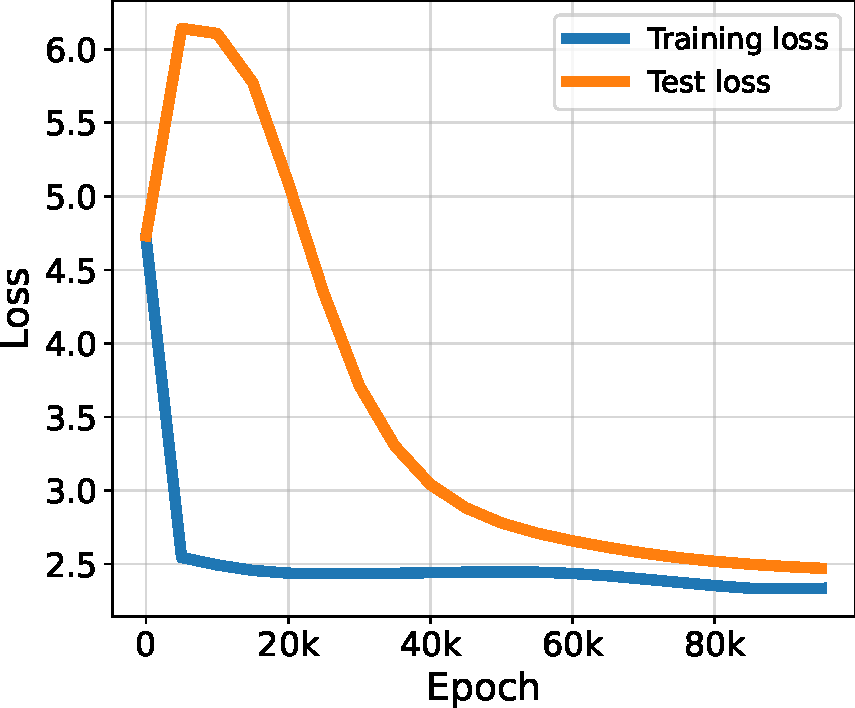
\includegraphics[width=\linewidth]{grokking_iclr_arxiv/figures/softermax_loss.pdf}
  \caption{$\stablemax$}
  \label{fig:additional_grokking_stablemax}
\end{subfigure}%
\hfill
\begin{subfigure}{.33\textwidth}
  \centering
  \includegraphics[width=\linewidth]{grokking_iclr_arxiv/figures/logit_reg_loss.pdf}
  \caption{Logit regularization}
  \label{fig:additional_grokking_logit}
  
\end{subfigure}%
\hfill
\begin{subfigure}{.33\textwidth}
  \centering
  \includegraphics[width=\linewidth]{grokking_iclr_arxiv/figures/taylor_loss.pdf}
  \caption{\tsoftmax}
  \label{fig:additional_grokking_taylor}
\end{subfigure}
\vspace{-3mm}
\caption{Train and test losses during grokking induced by three different interventions.\vspace{-2mm}}
\label{fig:additional_grokking}
\end{figure}

\begin{wrapfigure}[20]{R}{0.4\textwidth}
\vspace{-0.5cm}
    \centering
    \includegraphics[width=\linewidth]{grokking_iclr_arxiv/figures/fourier.pdf}
    \vspace{-6mm}
    \caption{Fourier components of the weights of the output layer of an MLP trained on addition mod 113. Grokking is induced via $\stablemax$ and without weight decay.}
    \label{fig:fourier}
\end{wrapfigure}
\noindent\textbf{Taylor approximation of the Softmax.}
We have introduced $\stablemax$ as a change to the \softmax that leads to grokking without regularization. The motivation behind this is to prevent values in the sum of the \softmax that are very large or very close to zero. To this end, replacing the exponential with any function that is sub-exponential beyond a certain point should have a similar effect. To demonstrate, we perform a further experiment using the second order Taylor approximation of the exponential 
\begin{equation}
e^x\approx \frac{1 + x + x^2}{2!},    
\end{equation}
replacing the $\exp$ in the \softmax. Since the Taylor approximation is decreasing for $x<0$, we subtract the minimum logit to avoid this part of the function.  We deem this version \tsoftmax.
In \cref{fig:additional_grokking} we see results similar to the ones in \cref{fig:stablemax_grokking} but showing the losses instead of the accuracies as well as results for two additional methods to induce grokking. 
Note that our implementation of \tsoftmax (\cref{fig:additional_grokking_taylor}) introduces an additional implicit regularization similar to the one in  \cref{fig:additional_grokking_logit}, due to the gradient flowing through the subtraction of the mean. % also introduces an additional regularization effect similar to the one 
While this effectively combines the effects of \cref{fig:additional_grokking_stablemax} and \cref{fig:additional_grokking_logit}, leading to grokking faster than the other two methods, our main paper shows results using $\stablemax$ as a cleaner intervention that does not introduce this additional regularization effect. 

% above \tolga{what is the 'one above'?}. This is why we show our main results using $\stablemax$ as a cleaner intervention that does not introduce this additional regularization effect. 

%Note that our implementation of \tsoftmax (\cref{fig:additional_grokking_taylor}) introduces an implicit regularization similar to the one in  \cref{fig:additional_grokking_logit}, effectively combining the effects of \cref{fig:additional_grokking_stablemax} and \cref{fig:additional_grokking_logit}, explaining why it leads to grokking faster than the other two methods. 






\subsection{Solution Learned During Grokking  Without Weight Decay}\label{app:fourier}

\begin{comment}
    \begin{wrapfigure}[20]{R}{0.4\textwidth}
            \vspace{-0.5cm}
            \begin{center}
    \includegraphics[width=0.4\textwidth]{grokking_iclr/figures/fourier_components.pdf}
            \end{center}
            \vspace{-10pt}
            \caption{Fourier components of the weights of the output layer of an MLP trained on addition mod 113. Grokking is induced with $\stablemax$ and without weight decay. \tolga{this figure is terribly cropped.}}
            \label{fig:fourier}
        \end{wrapfigure}
\end{comment}

 
Weight decay has been identified as potentially responsible for inducing the periodic structures in the weights studied in \cite{Nanda2023-hf}. In \cref{fig:fourier} we show that MLPs that grok without weight decay on modular addition show a similar sparsity in Fourier space as the one observed in \cite{Nanda2023-hf}. While these are very superficial results, they suggest that these structures can emerge without a weight decay--induced ``clean up'' phase as described in \cite{Nanda2023-hf}.

\section{Further Discussion on Conditions that Lead to Grokking}\label{app:further_discussion}
\subsection{L1 regularization and grokking}\label{app:l1_grokking}

%\paragraph{L1 regularization}
While it has been observed that L1 regularization can lead to grokking in some settings, \cite{Nanda2023-hf}
consistently found no grokking with L1 regularization and transformers and this setting has received substantially less attention than weight decay. 

We observe that \nlm scales the weights along their current direction. This means that larger weights are scaled more than small weights. However, while the sign of the gradient from L1 regularization depends on the sign of the weights, the magnitude of this gradient does not depend on the magnitude of the weights. This means that, particularly on deep networks or transformers with with large weights, L1 can sometimes be insufficient to prevent \nlm and the subsequent SC. 
%In Appendix \ref{app:l1_grokking} we show two examples, one where L1 regularization avoids SC and leads to grokking, and one where SC happens despite L1 regularization and grokking does not happen.

\subsection{Delaying generalization by scaling the weights} \label{app:scaling_weights}

\paragraph{Scaling the logits can delay generalization but not induce it} \cite{liu2023omnigrok}, \cite{Kumar2023-hz} and \cite{Lyu2023-ga} showed that an $\alpha$ parameter multiplying the logits can increase or reduce the delay in generalization. We highlight in \cref{fig:alpha_parameter} that this is true for cases where generalization happens even without changing the scale of the logits ($\alpha=1$). However, in most cases when using deeper networks or cross-entropy loss, models do not generalize by default without regularization and we are unable to induce grokking for any value of $\alpha$. 

We argue in \cref{sec:explain_existing_methods} that the observation in \cite{liu2023omnigrok}, \cite{Kumar2023-hz} and \cite{Lyu2023-ga} of grokking without regularization are due to the inductive bias of MSE loss which prevents NLM and leads to grokking in some settings for shallow networks.

\begin{figure}[t]
\centering
\begin{subfigure}{.33\textwidth}
  \centering
  \includegraphics[width=\linewidth]{grokking_iclr_arxiv/figures/one_layer_MSE_alpha_sweep.pdf}
  \caption{MSE: 1 hidden layer}
\end{subfigure}%
\hfill
\begin{subfigure}{.33\textwidth}
  \centering
  \includegraphics[width=\linewidth]{grokking_iclr_arxiv/figures/two_layer_MSE_alpha_sweep.pdf}
  \caption{MSE: 2 hidden layers}
\end{subfigure}%
\hfill
\begin{subfigure}{.33\textwidth}
  \centering
  \includegraphics[width=\linewidth]{grokking_iclr_arxiv/figures/two_layer_cross_entropy_alpha_sweep.pdf}
  \caption{CE: 2 hidden layers}
\end{subfigure}
\caption{The $\alpha$ parameter controls generalization in settings where it happens by default. This is the case for shallow networks with MSE loss as shown in subplot (a). However, in deeper networks (b) or networks with CE loss and no regularization (c), $\alpha$ can control the time of over-fitting, but no value of $\alpha$ is enough to trigger grokking.}
\label{fig:alpha_parameter}
\end{figure}

\paragraph{Grokking on MNIST} We replicate the setting from \cite{liu2023grokking} of grokking on MNIST with cross-entropy loss and show that without weight decay, the scaling factor of the weights leads to significant FP errors, preventing grokking from happening until this is alleviated by weight decay. 

While SC explains why weight decay is needed to get the jump in performance observed in \cref{fig:mnist}. It could also explain why inducing grokking by scaling the weights is less effective when using SCE. While when using MSE loss, \cite{liu2023omnigrok} are able to induce full grokking from random level predictions to close to full training accuracy, the same does not seem to be possible when using SCE. In fact, we see in \cref{fig:mnist} that since the begining of training the rate of SC approaches 100\%. This could explain why the observations with cross-entropy loss are not the ones predicted by the lazy training theories outlined in \cite{Kumar2023-hz} which do not take limited floating point precision into account.

\begin{figure}[t]
    \vspace{-6mm}
    \centering
    \begin{subfigure}{.48\textwidth}
    \includegraphics[width=\linewidth]{grokking_iclr_arxiv/figures/mnist_grokking.pdf}
        \caption{MLP without weight decay}
        \label{fig:mnist_witout_weight_decay}
    \end{subfigure}
    \begin{subfigure}{.48\textwidth}
    \includegraphics[width=\linewidth]{grokking_iclr_arxiv/figures/mnist_grokking_wd.pdf}
        \caption{MLP with weight decay.}
        \label{fig:mnist}
    \end{subfigure}
    \caption{Replicatting the grokking on MNIST for weight decay setting from \cite{liu2023grokking}. We find that MLPs with weights scaled up by 100 operate at the ``edge of numerical stability'' and in the absence of weight decay, SC eventually reaches 100\%, preventing any further generalization. When using weight decay, the weight norm is reduced, mittigating SC and eventually allowing for further generalization as the SC rate drops from 100\%.}

\end{figure}


\section{\ograd and Weight Decay}
In \cref{fig:wd_vs_ortho}, we provide a more in depth comparison of \ograd and weight decay. \cref{fig:wd_sweep} higlights that increasing the weight decay multiplier leads to a smaller delay in generalization, but only up to a point. In this concrete setting, a weight decay multiplier of 8, prevents the model from fully generalizing (\cref{fig:wd_sweep}). We then compare the best value of weight decay in this setting to \ograd, which does not require any hyper-parameter tuning. \cref{fig:vs_wd_seeds} shows that \ograd leads to faster grokking even when compared to a tuned value of weight decay. Note that the models with weight decay overfit immediately before grokking while \ograd reaches 100\% train and test accuracies almost at the same time.


\begin{figure}[t]
    \vspace{-5mm}
    \centering
    \begin{subfigure}{.48\textwidth}
    \includegraphics[width=\linewidth]{grokking_iclr_arxiv/figures/weight_decay_sweep.pdf}
        \caption{Sweep over values of weight decay}
        \label{fig:wd_sweep}
    \end{subfigure}
    \begin{subfigure}{.48\textwidth}
    \includegraphics[width=\linewidth]{grokking_iclr_arxiv/figures/weight_decay_vs_orthograd_seeds.pdf}
        \caption{\ograd vs best performing wd model}
        \label{fig:vs_wd_seeds}
    \end{subfigure}
    \caption{Increasing weight decay (WD) for an MLP trained on modular addition with AdamW reduces the delay in generalization up to a point where WD prevents convergence \cref{fig:wd_sweep}. Without any tunable hyper-parameters and without WD, \ograd leads to grokking faster than the best model with WD \cref{fig:vs_wd_seeds}.}
    \label{fig:wd_vs_ortho}
\end{figure}

\section{Alternatives to $\stablemax$ in Preventing SC}
\begin{wrapfigure}[15]{R}{0.45\textwidth}
    \vspace{-7mm}
    \includegraphics[width=\linewidth]{grokking_iclr_arxiv/figures/label_smoothing.pdf}
    \vspace{-8mm}
    \caption{$\stablemax$ prevents SC and leads to grokking while temperature scaling with $T=1e5$ only gradually delays SC, and label smoothing does prevent SC but at the cost of keeping the model from fully generalizing.}
    \label{fig:label_smoothing}
\end{wrapfigure}
While any intervention that prevents SC should lead to grokking or generalization, \cref{fig:label_smoothing} shows that scaling the temperature of the \softmax is not enough to prevent SC and label smoothing does prevent SC and lead to some generalization, but at the cost of introducing another inductive bias that prevents full generalization and leads to qualitatively different behavior. By comparison, the simple change introduced in Stablemax prevents SC and leads to grokking, serving as a validation for our hypothesis that gradient descent leads to grokking by default, unless this is stopped by SC.



\section{$\stablemax$ and \ograd \\ in Realistic Settings}
While Stablemax and \ograd are designed as interventions to show that preventing SC leads to grokking and preventing NLM leads to generalization (\cref{fig:teaser}), in this section we explore if these methods are applicable in more realistic settings like language modeling with GPT2-small or ResNets trained on image classification. We train GPT2-Small for 1 epoch on WikiText-103 using a batch size of 16, a block size of 512, a learning rate of $5e-4$ and a weight decay of 0.01 using AdamW. The architecture is the regular GPT2-Small architecture from \cite{radford2019language}, trained with a cosine schedule and 1000 steps of warmup.

For CIFAR10, CIFAR100 and Imagenet-1k \citep{ILSVRC15}, our baseline is a ResNet18 with SCE loss trained with SGD 0.9 momentum and $1e-4$ weight decay. We use standard data transformations such as random crop and random horizontal flip and a step learning rate scheduler every 30 epochs for a full training run of 100 epochs. With respect to this baseline we report results replacing the $\softmax$ with $\stablemax$ in the loss function, as well as replacing SGD with $\perp$SGD. Since test labels for Imagenet-1k are not publicly available, we use the validation set as a test set and tune hyper-parameters on a fraction of the training set.


\begin{figure}[t]
    \centering
    \begin{subfigure}{.32\textwidth}
    \includegraphics[width=\linewidth]{grokking_iclr_arxiv/figures/gpt2-small.pdf}
        \caption{GPT2-Small on WikiText2}
        \label{fig:gpt2_small}
    \end{subfigure}
    \hfill
    \begin{subfigure}{.32\textwidth}
    \includegraphics[width=\linewidth]{grokking_iclr_arxiv/figures/CIFAR100.pdf}
        \caption{ResNet18 on CIFAR100}
        \label{fig:cifar100_resnet18}
    \end{subfigure}
    \hfill
    \begin{subfigure}{.32\textwidth}
    \includegraphics[width=\linewidth]{grokking_iclr_arxiv/figures/cifar10_resnet18.pdf}
        \caption{ResNet18 on CIFAR10}
        \label{fig:cifar10_resnet18}
    \end{subfigure}
    \caption{Comparing Stablemax and \ograd to AdamW with SCE on text data \cref{fig:gpt2_small} and image data \cref{fig:cifar10_resnet18}. For the GPT2-small results in \cref{fig:gpt2_small}, we also include the results of replacing the \softmax in the attention mechanism with $\stablemax$.}
\end{figure}

\begin{table}[h]
\centering
\begin{tabular}{@{}lcccc@{}}
\toprule
\textbf{Method}         & \textbf{CIFAR10} & \textbf{CIFAR100} & \textbf{ImageNet-1k} & \textbf{WikiText-103} (Top-5) \\ \midrule
Softmax CE              & $87.17\% \pm 0.2$ & $59.98\% \pm 0.4$  & $69.33\% \pm 0.04$              & $60.48\% \pm 0.04$                      \\
Stablemax CE            & $87.01\% \pm 0.2$ & $60.63\% \pm 0.4$  & $65.87\% \pm 0.22$             & $51.85\%  \pm 0.47$                  \\
\ograd                  & $87.22\% \pm 0.2$ & $62.69\% \pm 0.1$  & $68.95\% \pm 0.03$               & $59.64\%   \pm 0.04$                \\ 
\midrule
Stablemax Attention     & --                & --                 & --                   & $58.52\%   \pm 0.04$                   \\ \bottomrule
\end{tabular}
\label{tab:realistic_datasets}
\caption{For the methods introduced in this paper, we report accuracies with standard deviations across five seeds for the CIFAR datasets and three seeds for Imagenet-1k and WikiText-103. We report Top-5 accuracy in the case of WikiText-103.\vspace{-3mm}}
\end{table}


\section{SC and the Slingshot Effect}\label{app:slingshots}
\cite{slingshot-mechanism} observed that spikes in the training loss appear when training on grokking tasks with adaptive optimizers like Adam, and that these spikes can lead to generalization without weight decay. Although \cite{Nanda2023-hf} showed that slingshots are not necessary for grokking, it is still unclear what mechanism of adaptive gradient optimizers induces this behavior and why it leads to generalization. In light of the results in this paper, we believe that slingshots could lead to generalization because they prevent full SC. \cite{Nanda2023-hf} pointed out that something like SC could be responsible for these slingshots. One possible mechanism would be that zero gradients for some samples due to SC rapidly diminish the second-order moments leading to a large update or slingshot which moves the model away from full SC, although more research would be needed to properly show this.

While related to our work, slingshots are a different kind of instability which only appears with adaptive optimizers and can allow grokking. In contrast, we identify SC as a very specific issue in the \softmax that can affect any model trained with SCE, not only the ones trained with adaptive optimizers. Additionally SC prevents grokking whereas slingshots can lead to it. Wether and how slingshots are cause by SC remains an open research question, with some supporting evidence from \cite{Nanda2023-hf} which show that slingshots can disappear when using $float64$.

\section{Additional Details About Floating Points}
Beyond our main results, we found that in some cases, grokking could be stopped before SC due to the $\epsilon$ parameter in Adam being too large. While the $\epsilon$ term is designed to give numerical stability to the gradients, in settings with extremely low losses and gradients, the second order moments can be dominated by the $\epsilon$ term, putting an end to learning where it would have continued with a smaller $\epsilon$ value. This echoes the results in \cite{slingshot-mechanism} which shows that increasing $\epsilon$ halts slingshots and grokking, with \cite{Nanda2023-hf} also alluding to the $\epsilon$ parameter being important in some cases.  

Surprisingly, we also found that a simple re-implementation of $torch.nn.functional.log\_softmax$ that does not use the official CUDA kernels can lead the models to keep learning beyond the point where the loss is exactly 0 and some gradients should be 0 with appropriate calculation, outperforming the official implementation for grokking tasks. Learning eventually also stops in this setting and this seems more like a quirk of how gradients are calculated in PyTorch in the absence of an explicitly defined backward pass.




%%%%%% for arxiv %%%%%% 

\end{sloppypar}
\end{document}
\endinput
%%
%% End of file `sample-sigconf-authordraft.tex'.
